\chapter[Signal and background predictions][Signal and background predictions]{Signal and background predictions}
\label{chap:backgrounds}

\begin{quote}
The modeling of relevant physics processes in the $\Htautau$ analysis are described.
\end{quote}

\section{$\Ztautau$}
\label{sec:backgrounds-ztautau}

\subsection{Mis-modeling of $\Zjets$ in simulation}

\begin{figure}[tp]
  \centering
  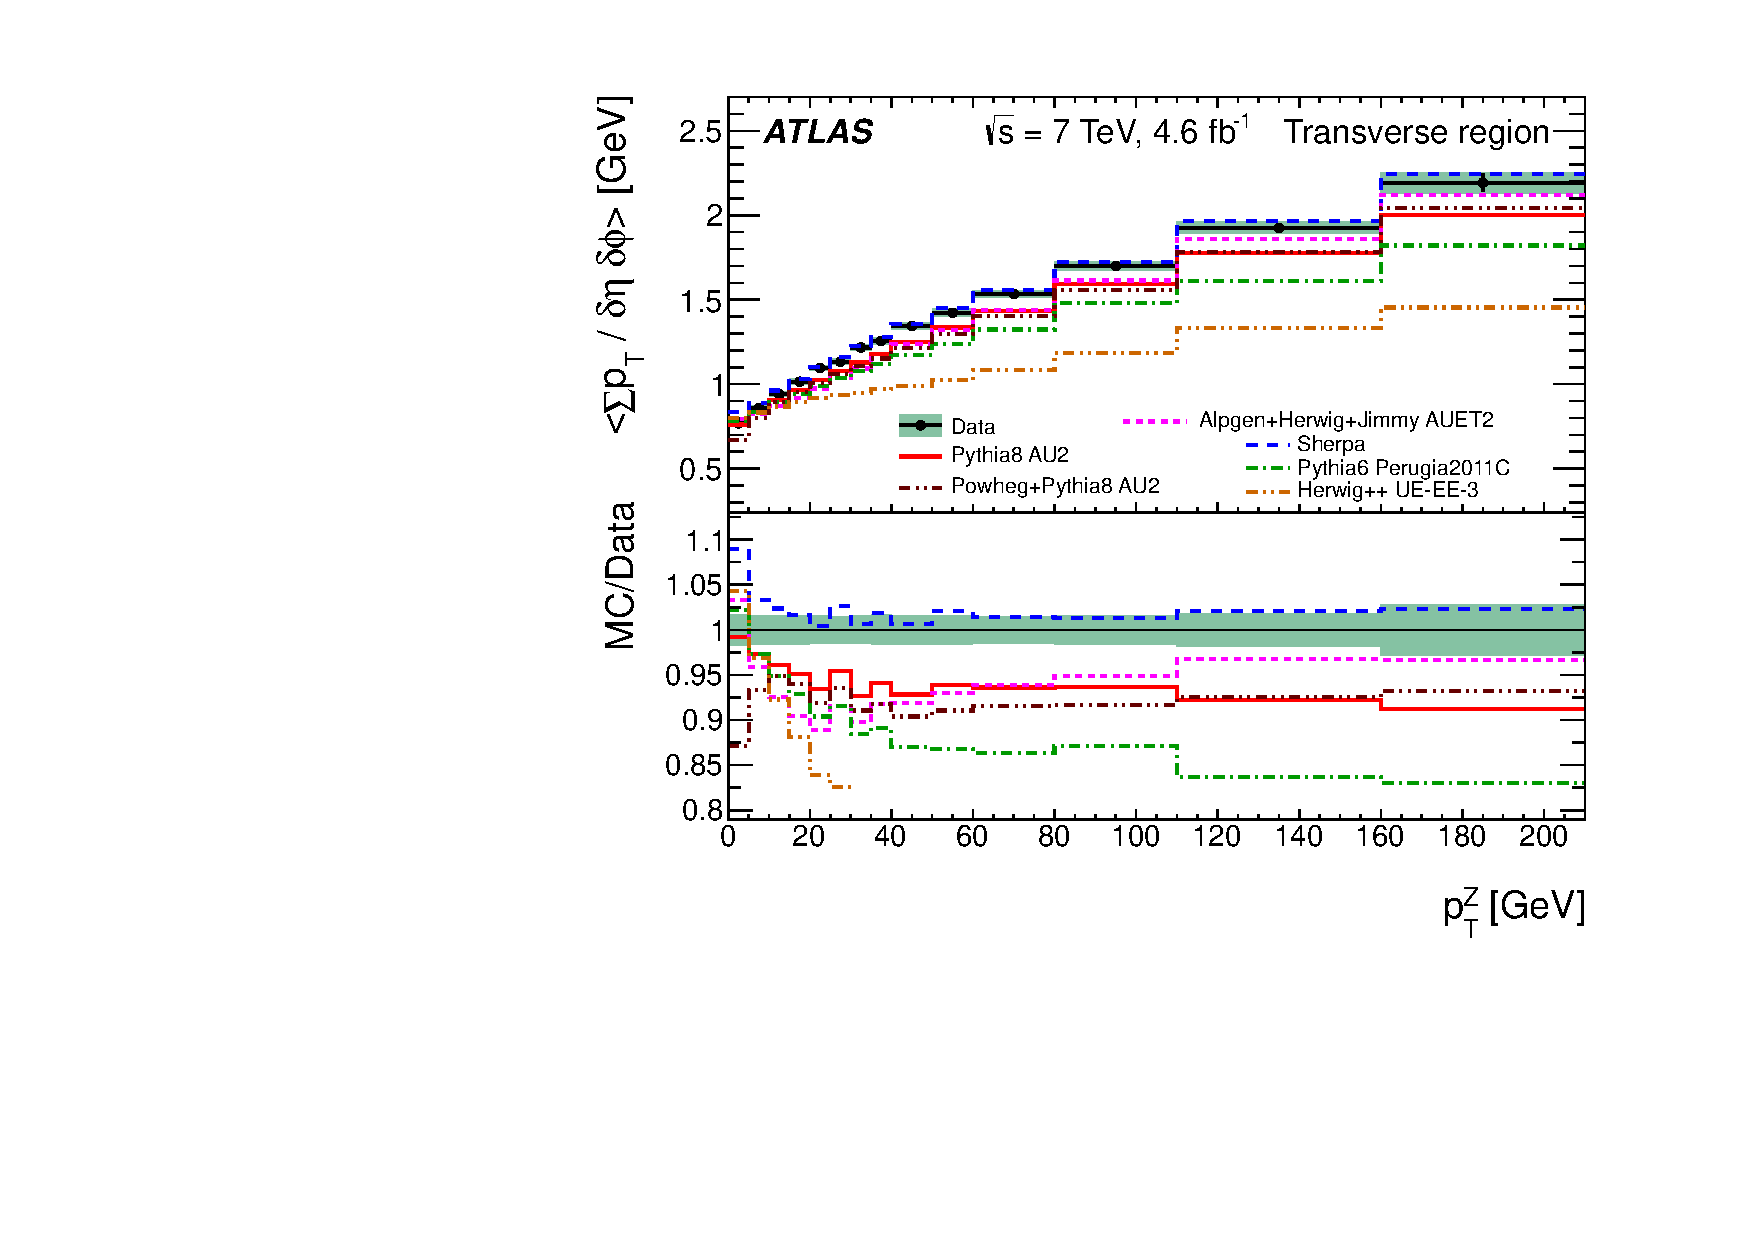
\includegraphics[width=0.48\textwidth]{figures/STDM-2011-42/fig_14b}
  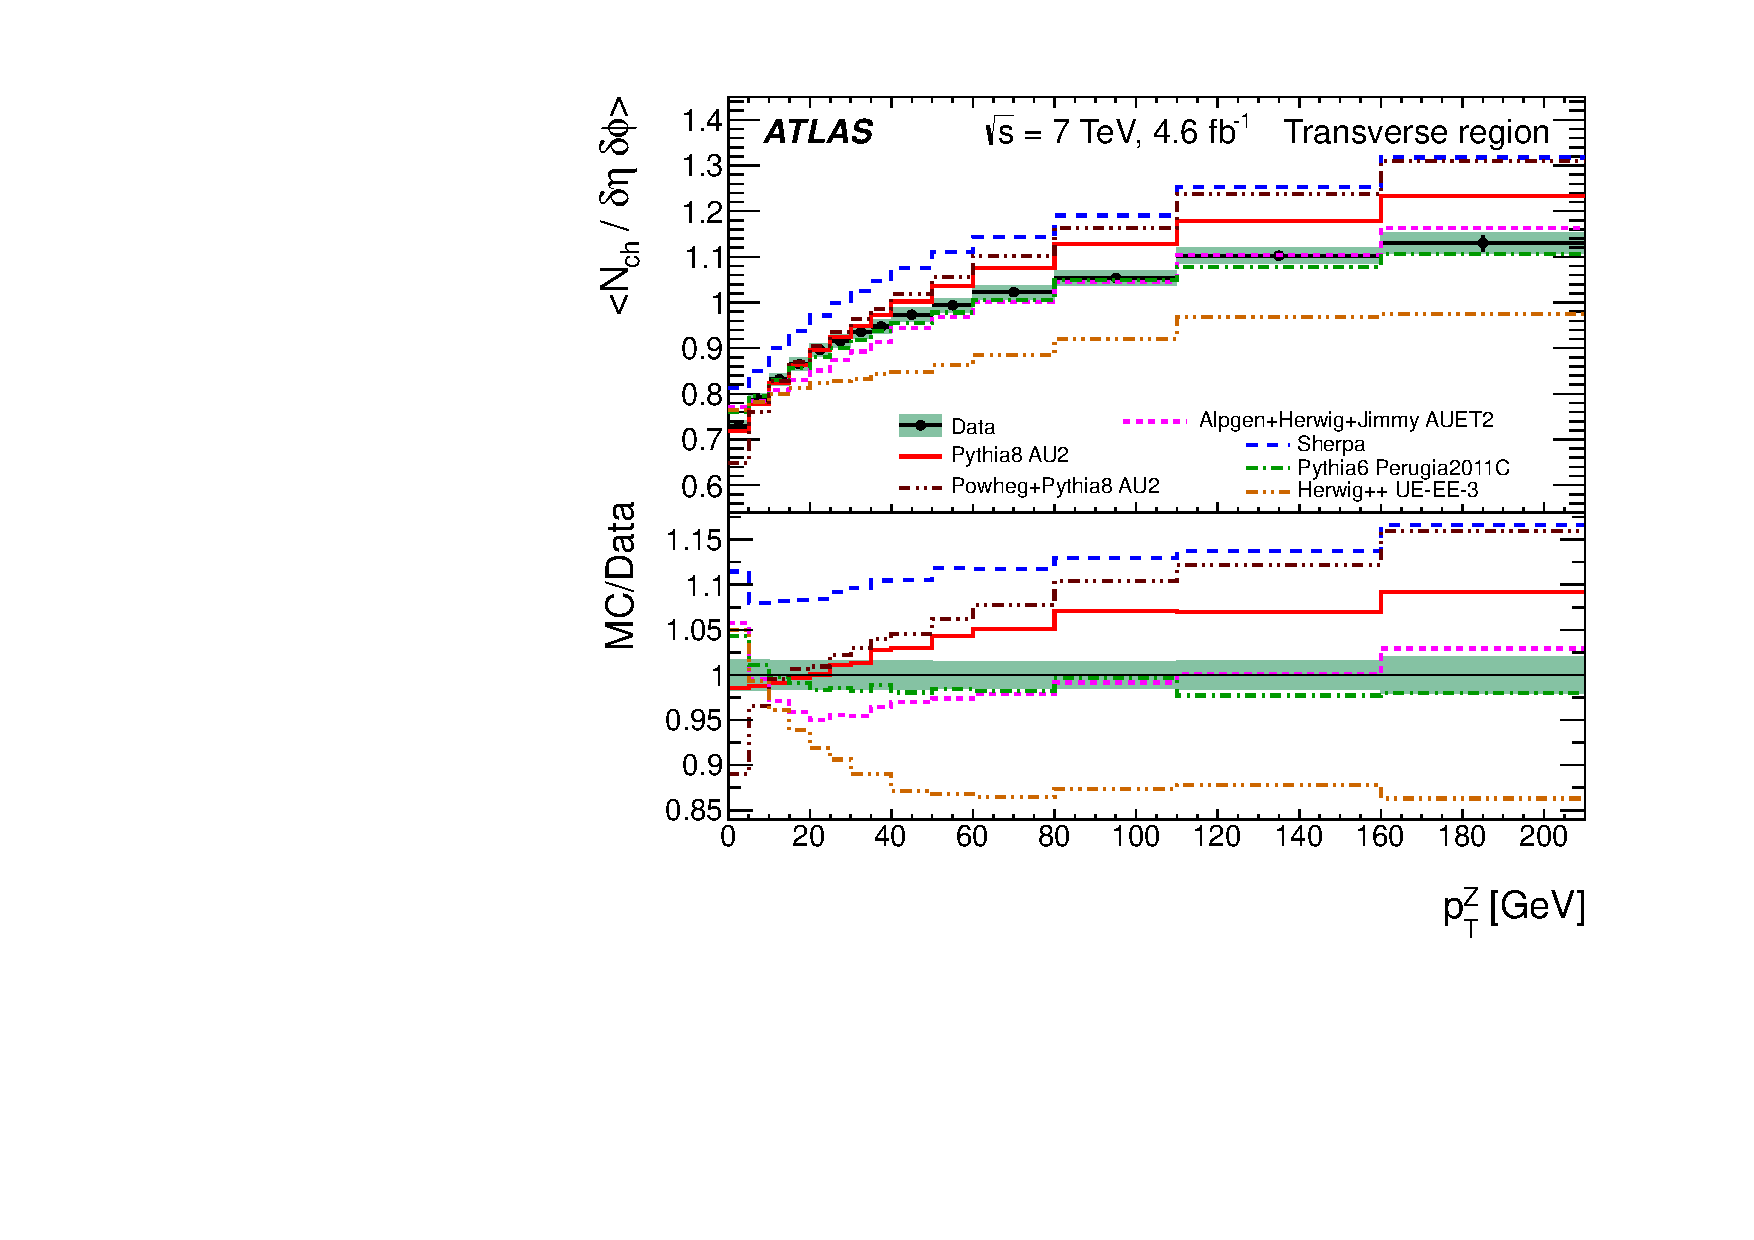
\includegraphics[width=0.48\textwidth]{figures/STDM-2011-42/fig_17b}
  \caption{Comparison of data and various predictions in $\Zll$ events of the charged particle scalar momentum density (left) and multiplicity density (right) as a function of $\pt^Z$ in 2011 data-taking. Mis-modeling is observed for all predictions.}
  \label{fig:backgrounds-zue}
\end{figure}

\begin{figure}[tp]
  \centering
  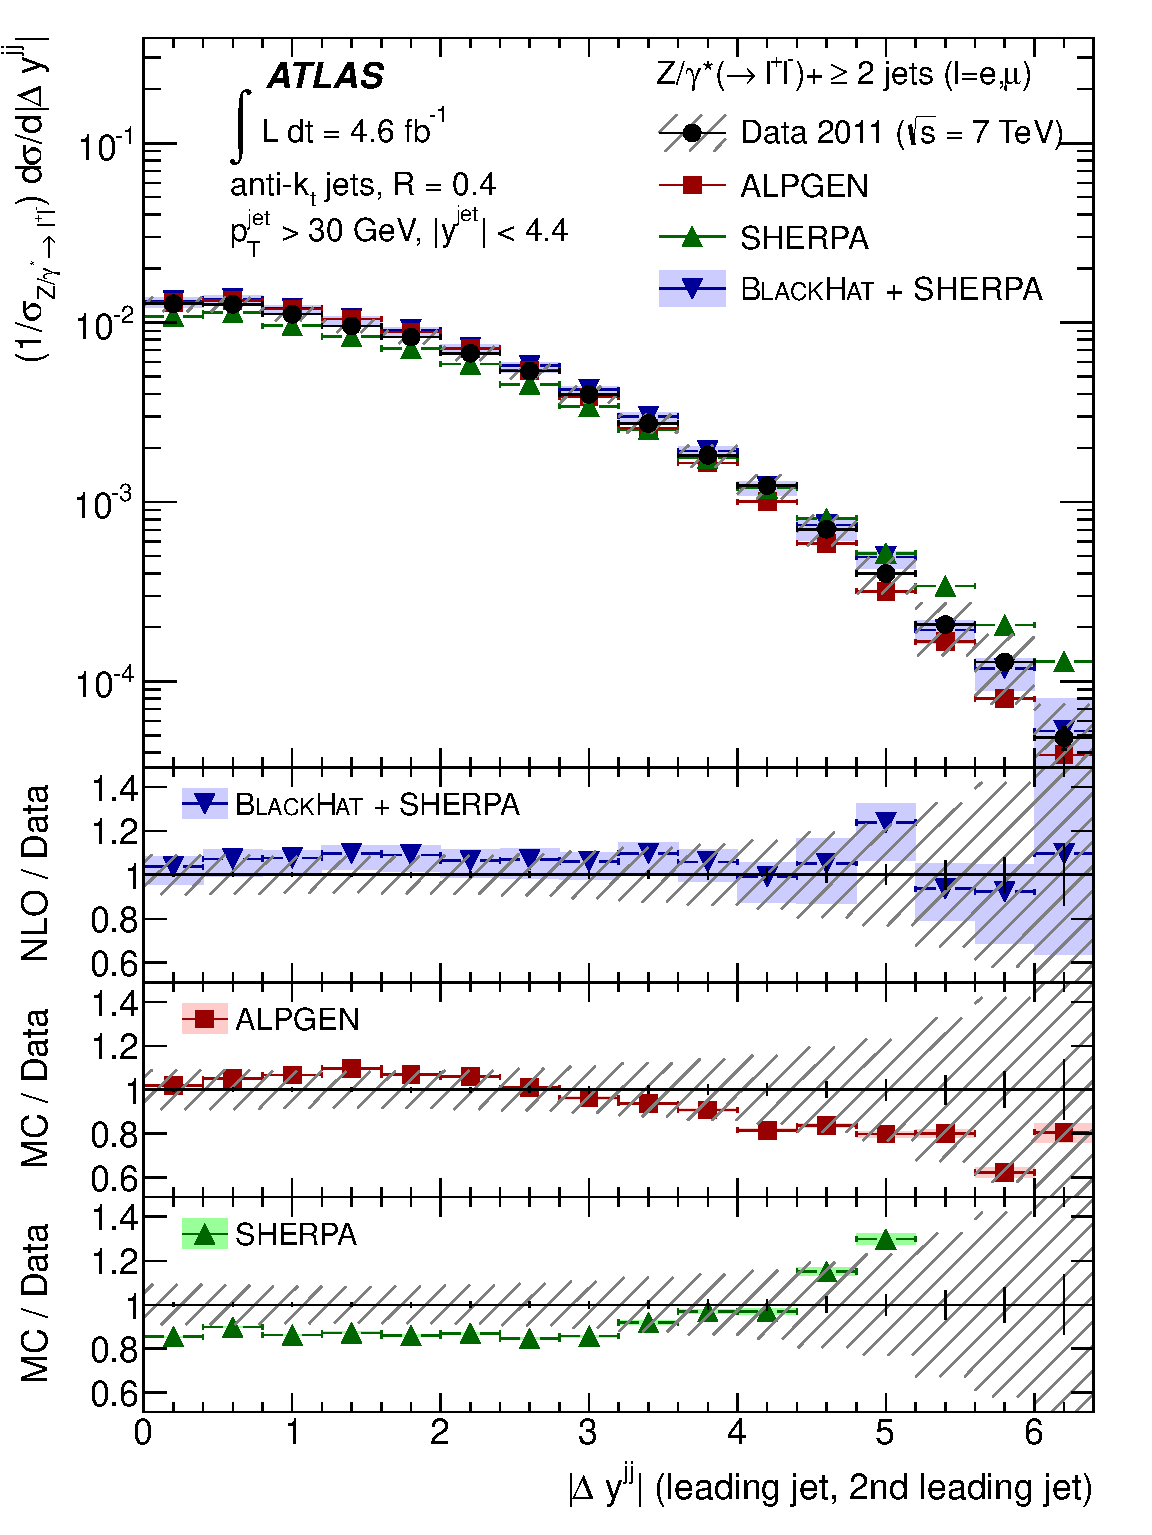
\includegraphics[width=0.48\textwidth]{figures/STDM-2012-04/fig_11a}
  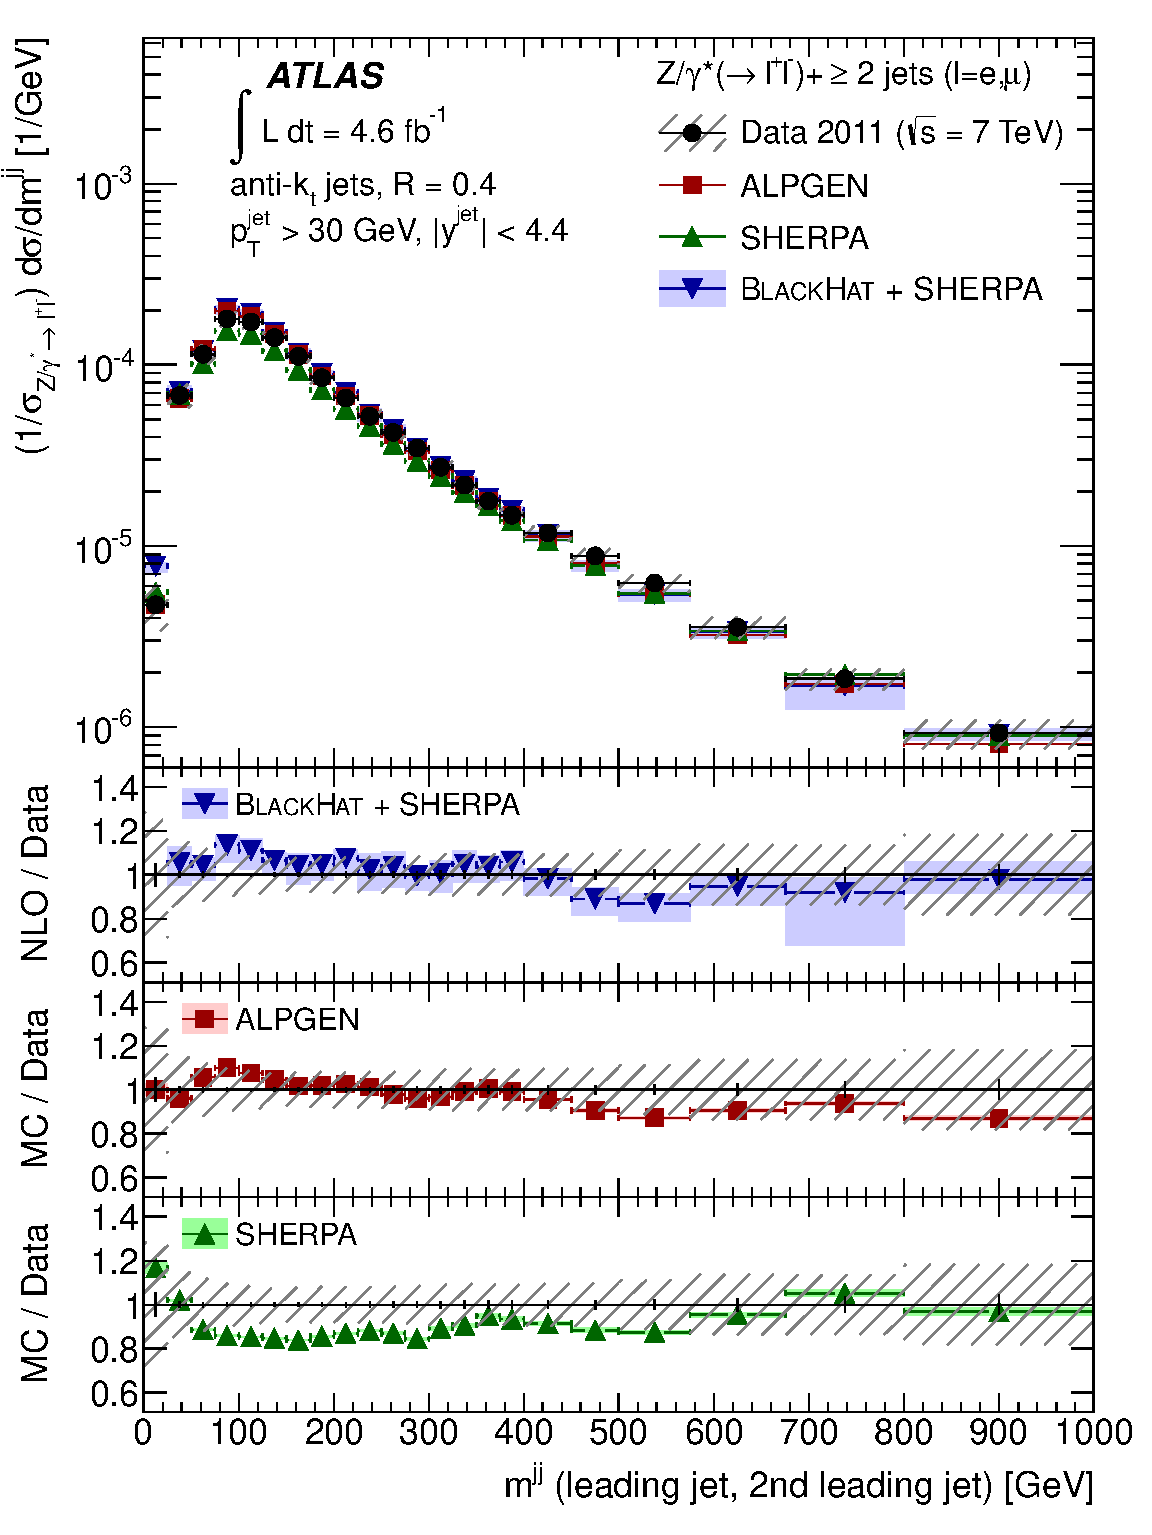
\includegraphics[width=0.48\textwidth]{figures/STDM-2012-04/fig_11b}
  \caption{Comparison of data and various predictions in $\Zll$ events of $\Delta Y(jj)$ (left) and $\mjj$ (right) in 2011 data-taking. Mis-modeling is observed for all predictions.}
  \label{fig:backgrounds-zjj}
\end{figure}

\begin{figure}[tp]
  \centering
  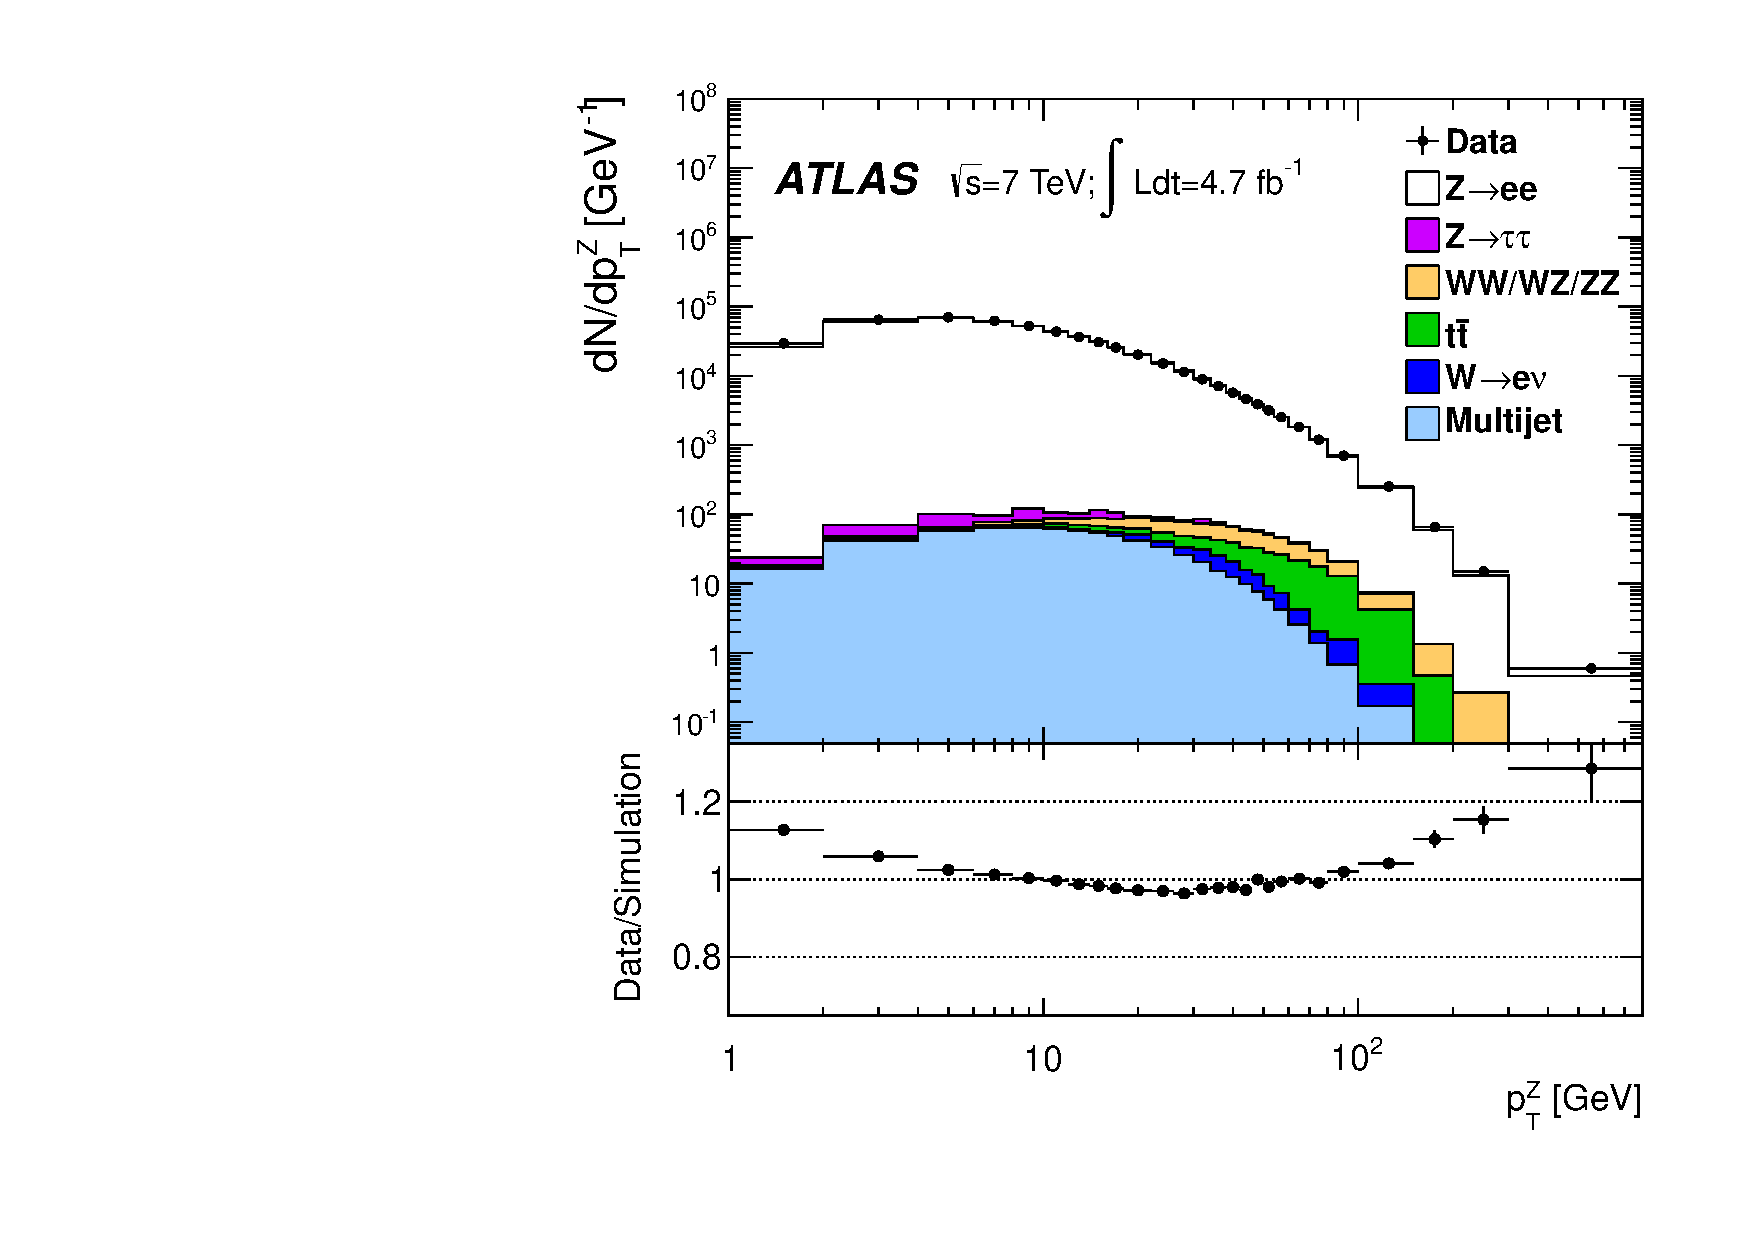
\includegraphics[width=0.48\textwidth]{figures/STDM-2012-23/fig_01a}
  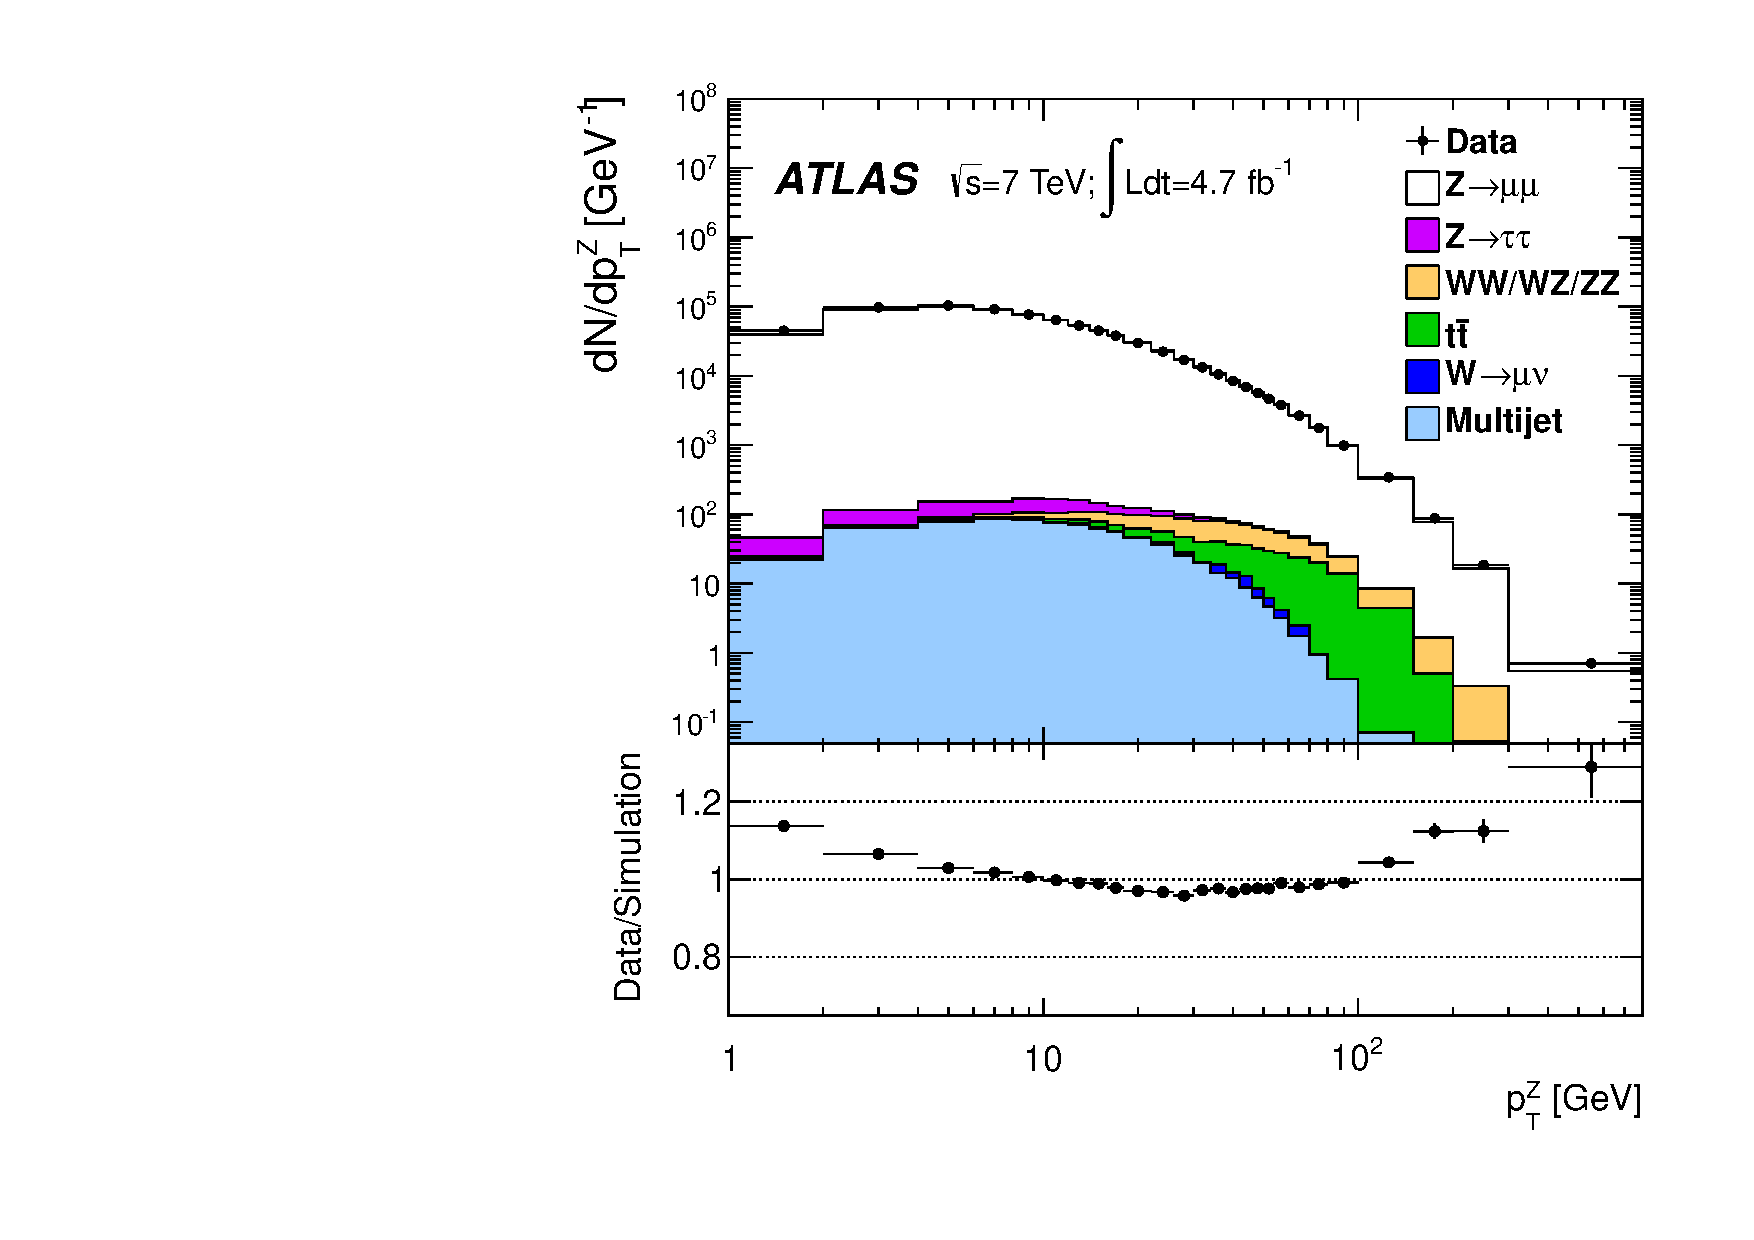
\includegraphics[width=0.48\textwidth]{figures/STDM-2012-23/fig_01b}
  \caption{Comparison of data and various predictions of $\pt^Z$ for $\Zee$ (left) and $\Zmm$ (right) in 2011 data-taking. Mis-modeling is observed for all predictions.}
  \label{fig:backgrounds-zpt}
\end{figure}

\subsection{Embedding}

\subsection{Validation}

\begin{figure}[tp]
  \centering
  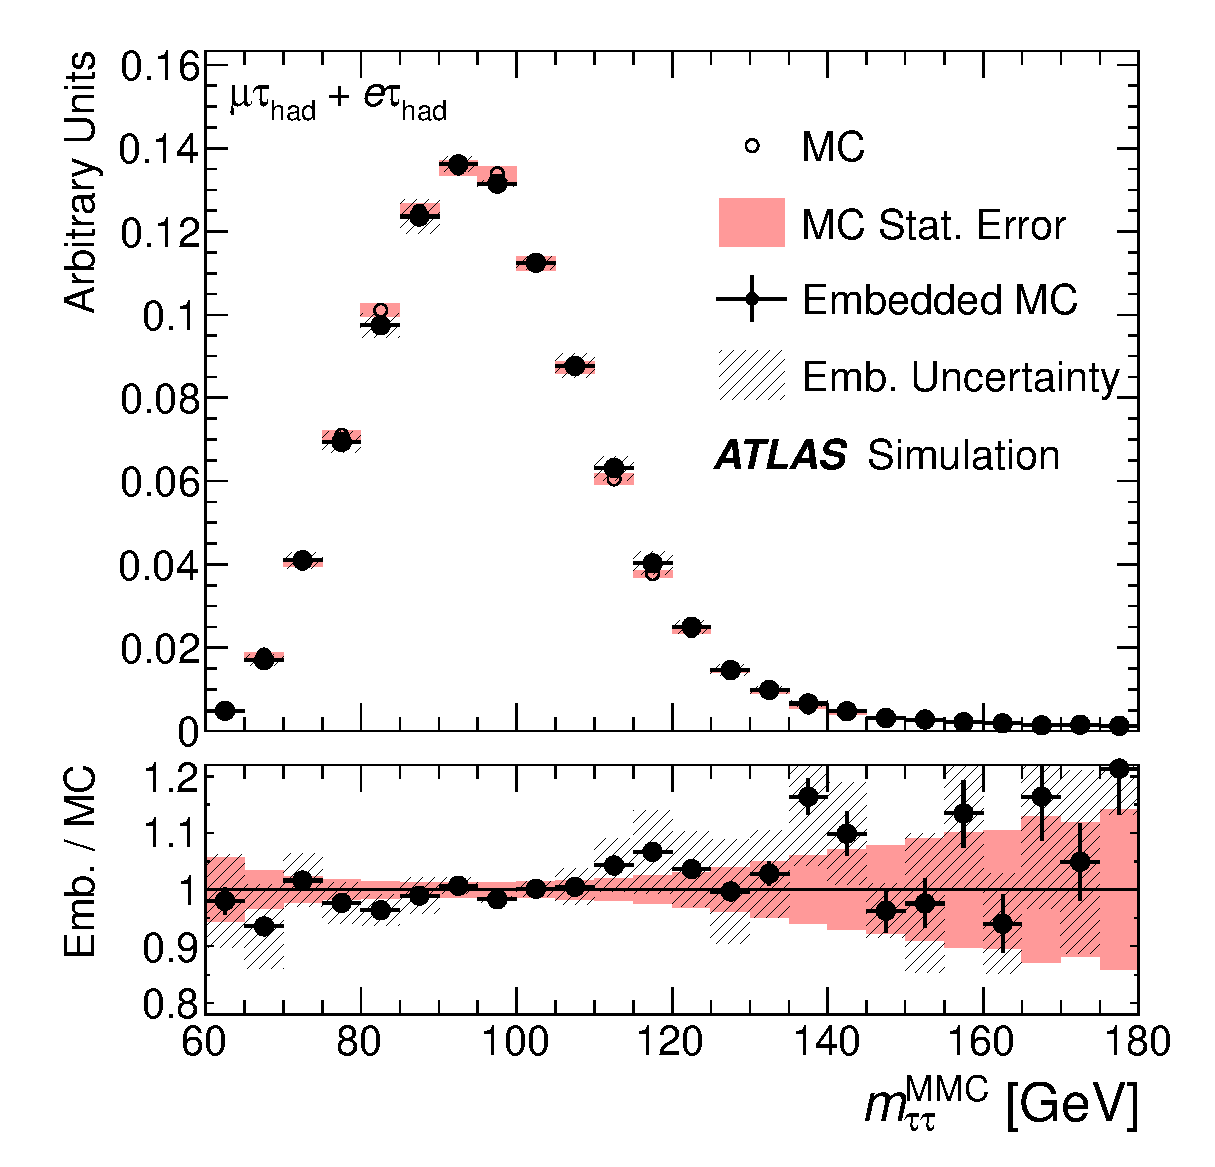
\includegraphics[width=0.48\textwidth]{figures/HIGG-2013-32/fig_03b}
  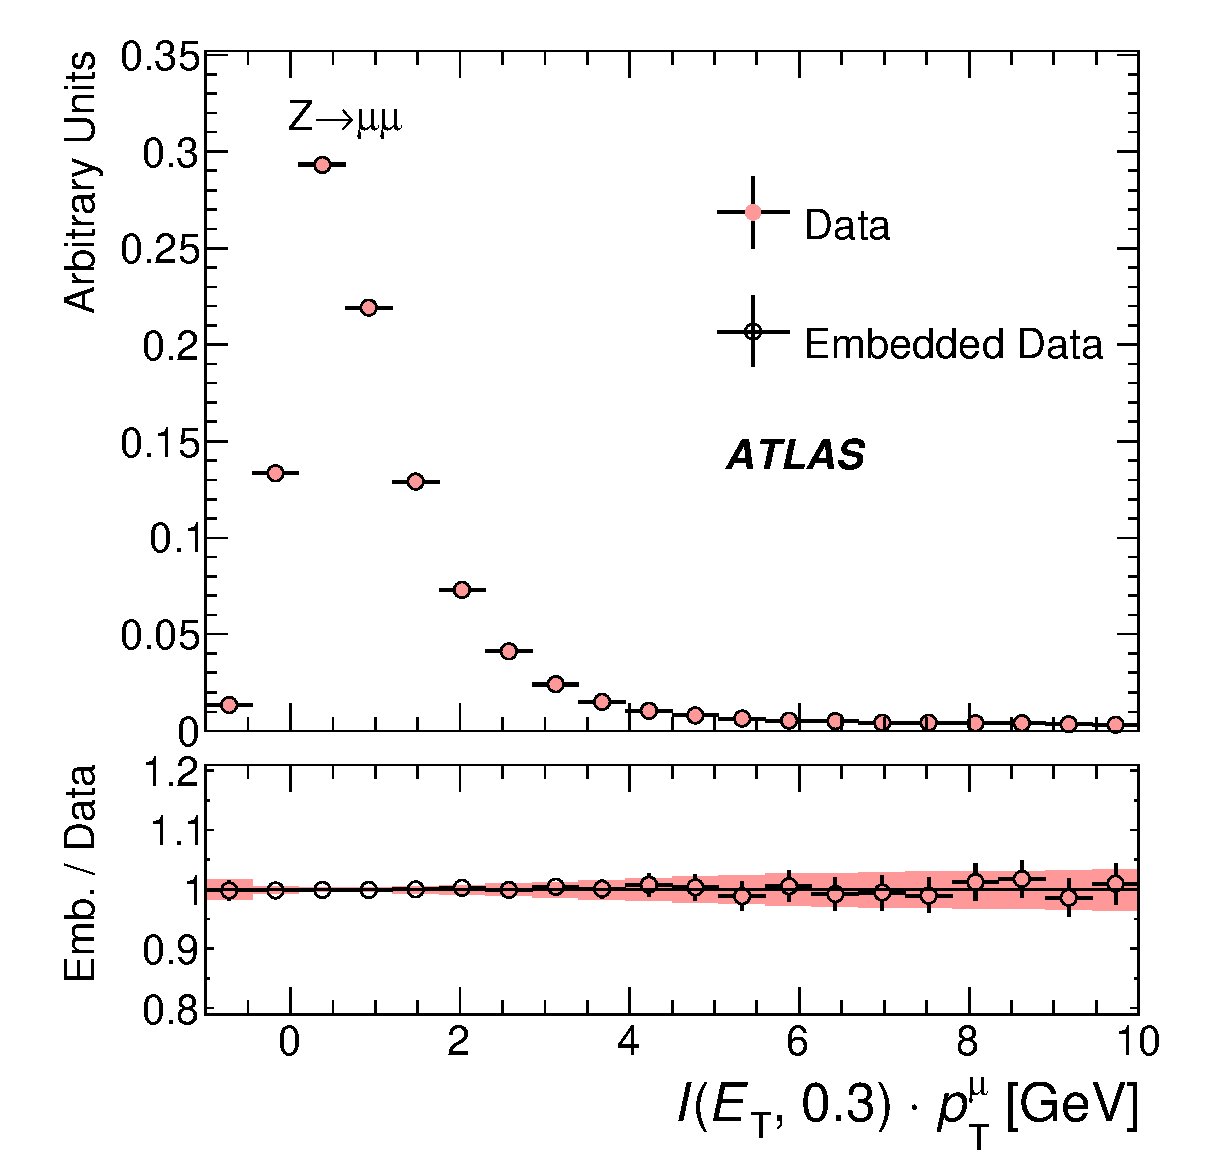
\includegraphics[width=0.48\textwidth]{figures/HIGG-2013-32/fig_03a}
  \caption{Validation of the embedding technique for simulated tau lepton decays in simulated $\Zmm$ events (left) and simulated muons in data $\Zmm$ events (right). Good agreement is observed in both.}
  \label{fig:backgrounds-embedding-validation}
\end{figure}

\clearpage

\subsection{Uncertainties}

\begin{figure}[tp]
  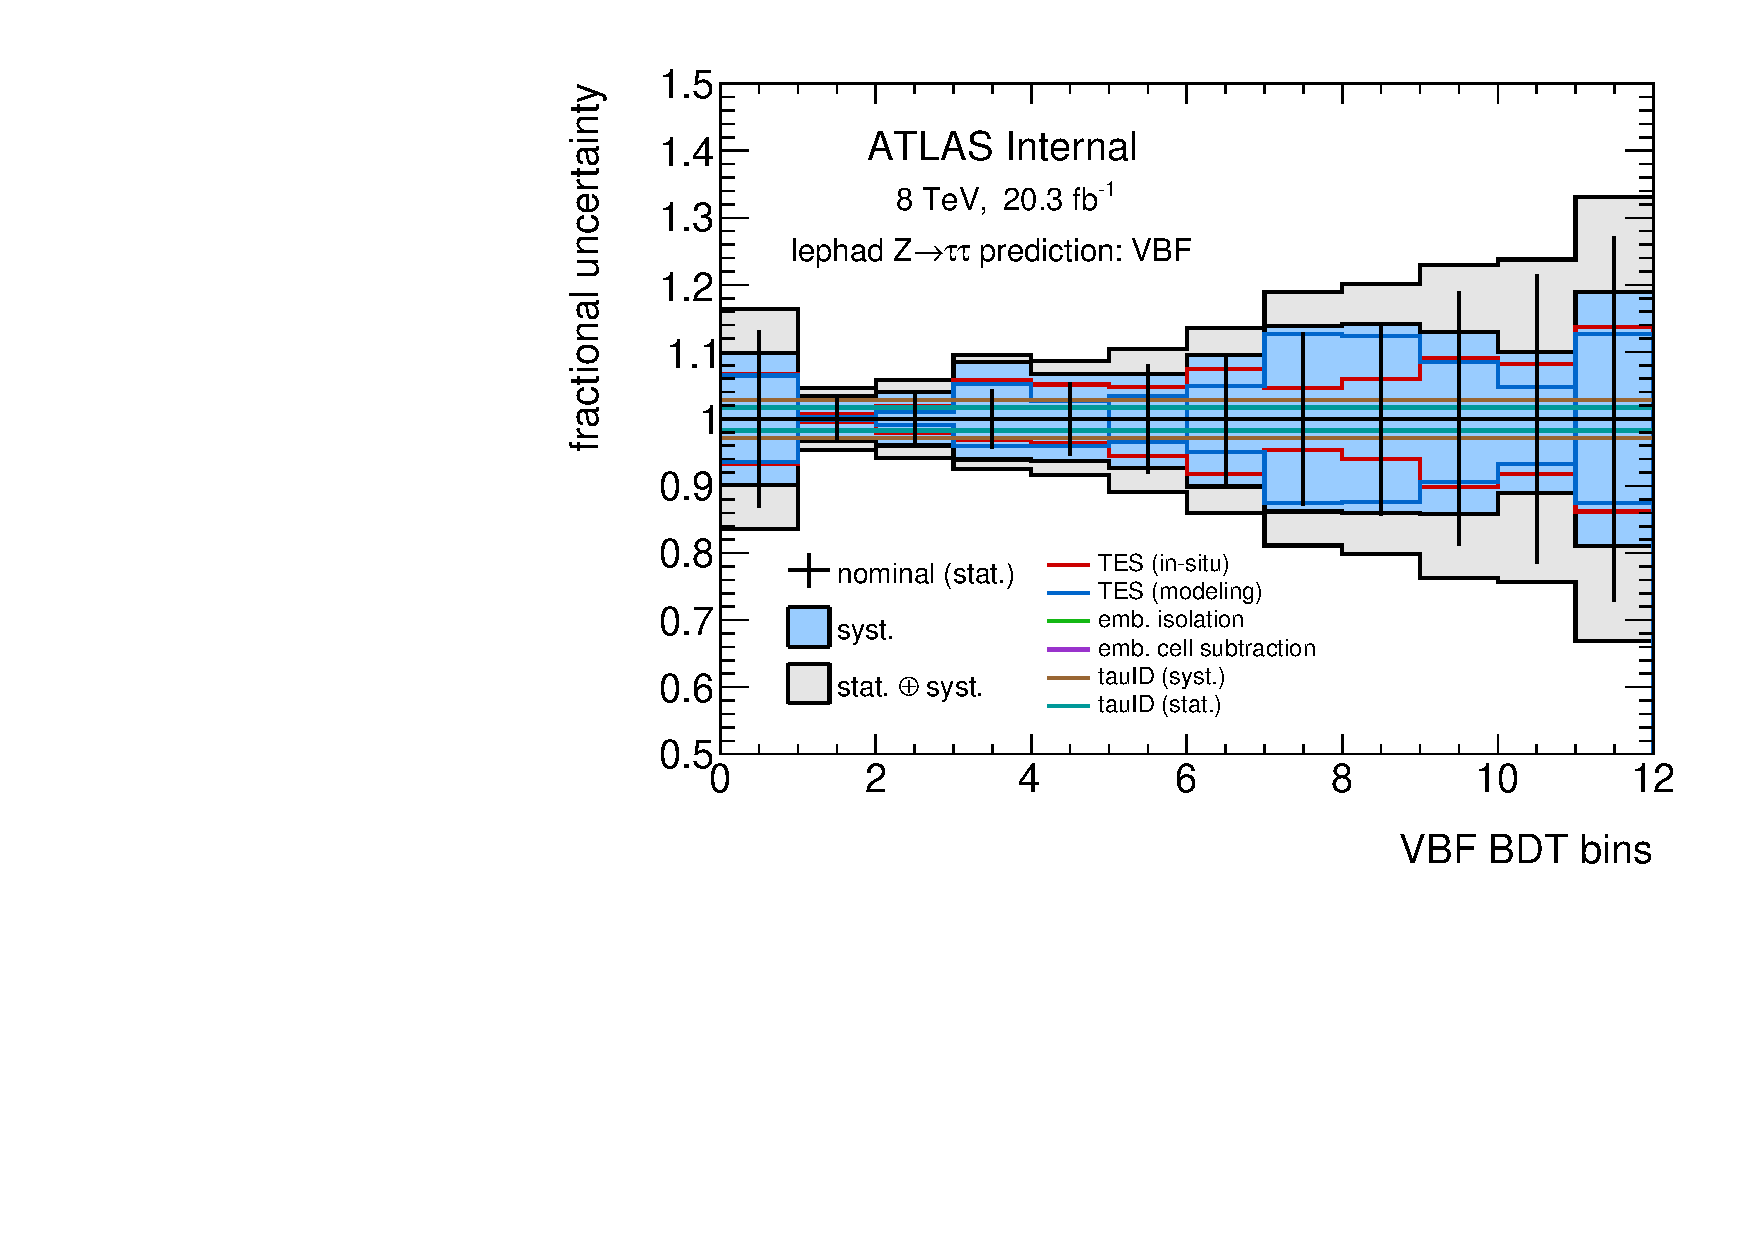
\includegraphics[width=0.90\textwidth]{figures/uncertainties/uncertainties_lephad_paper14_8TeV_Ztautau_VBF}
  \caption{The fractional uncertainty on the embedded $\Ztautaulh$ prediction in each bin of the VBF category for uncertainties pertaining to the embedding procedure and $\tauh$ performance.}
  \label{fig:backgrounds-uncertainties-Ztautau}
\end{figure}

\clearpage
\section{$\fakes$ mis-identification}
\label{sec:backgrounds-misid}

\subsection{Mis-modeling of $\fakes$ in simulation}

\subsection{Fake factor method}

\begin{figure}[tp]
  \centering
  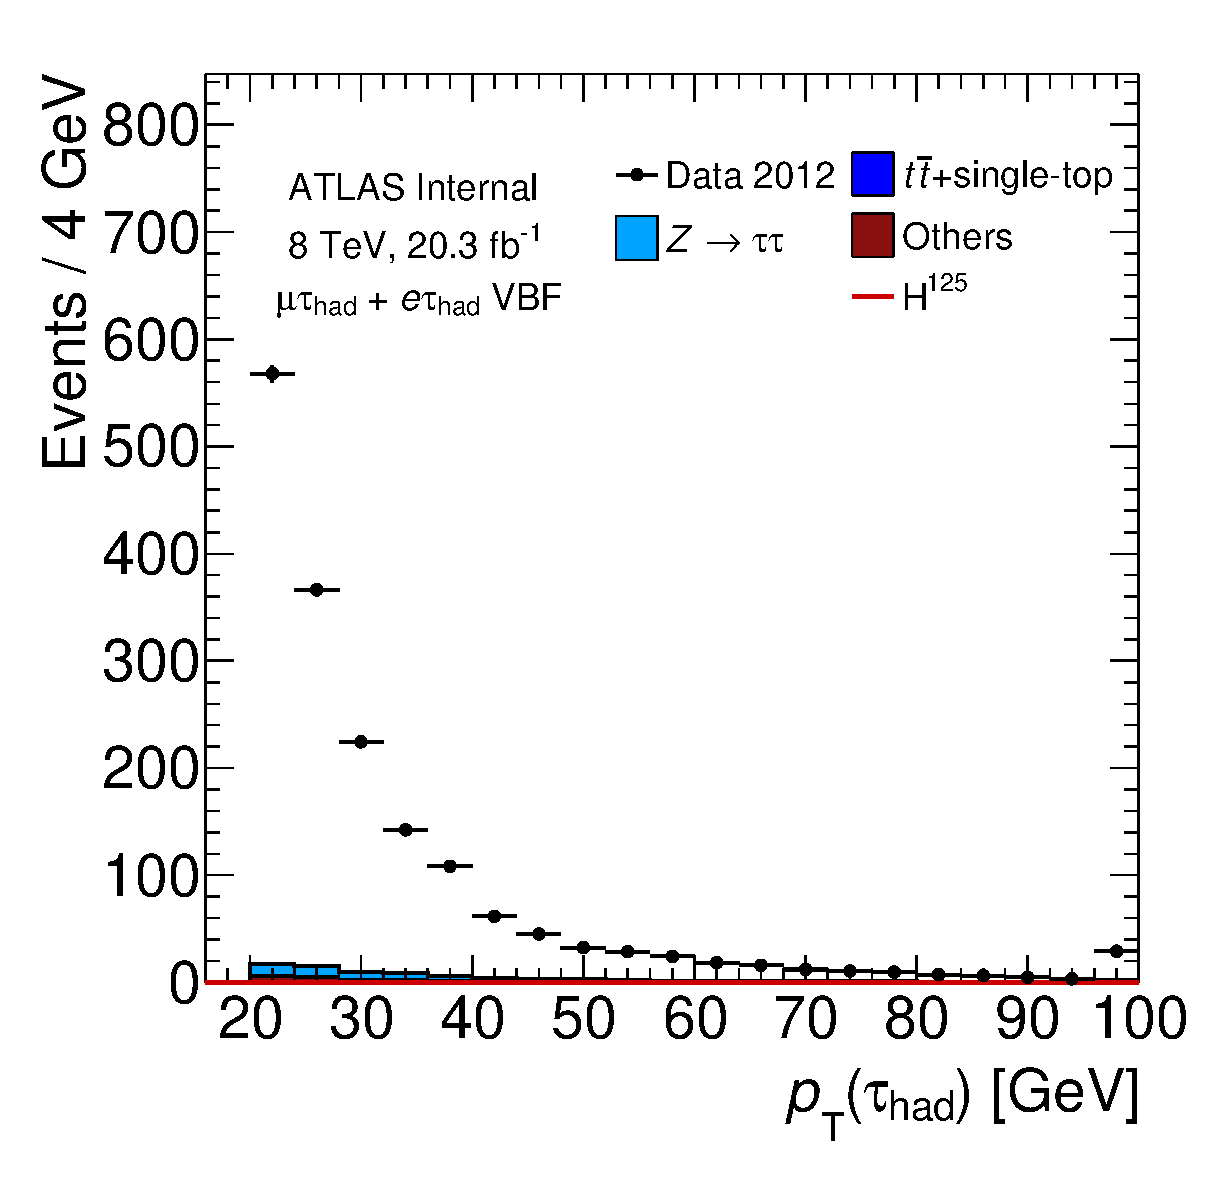
\includegraphics[width=0.32\textwidth]{figures/antitaus/tau-pt}
  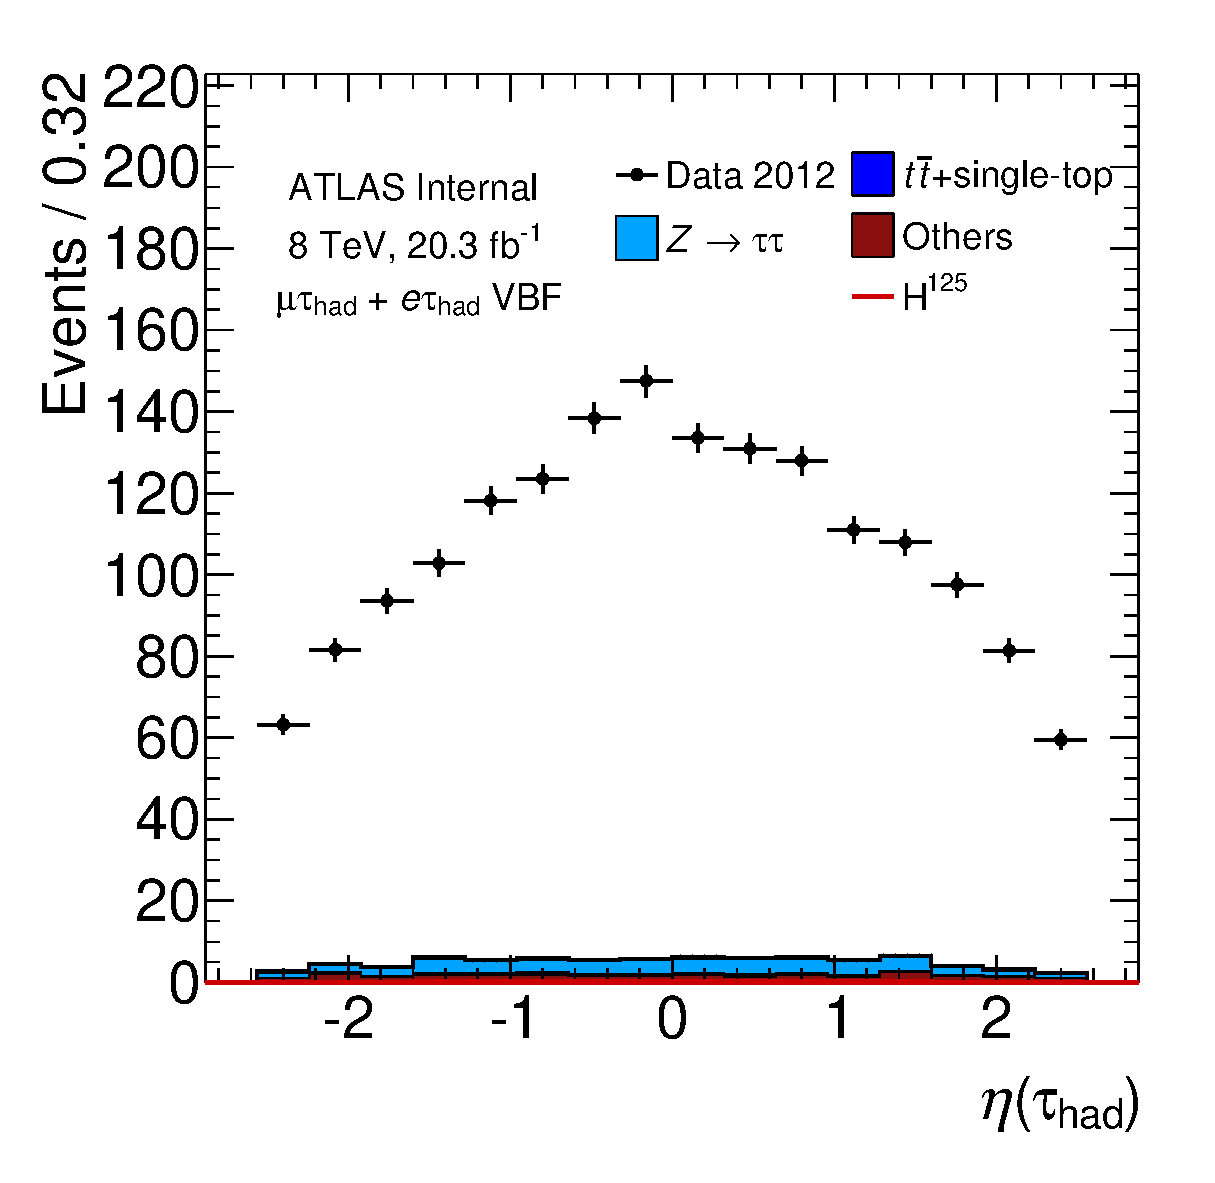
\includegraphics[width=0.32\textwidth]{figures/antitaus/tau-eta}
  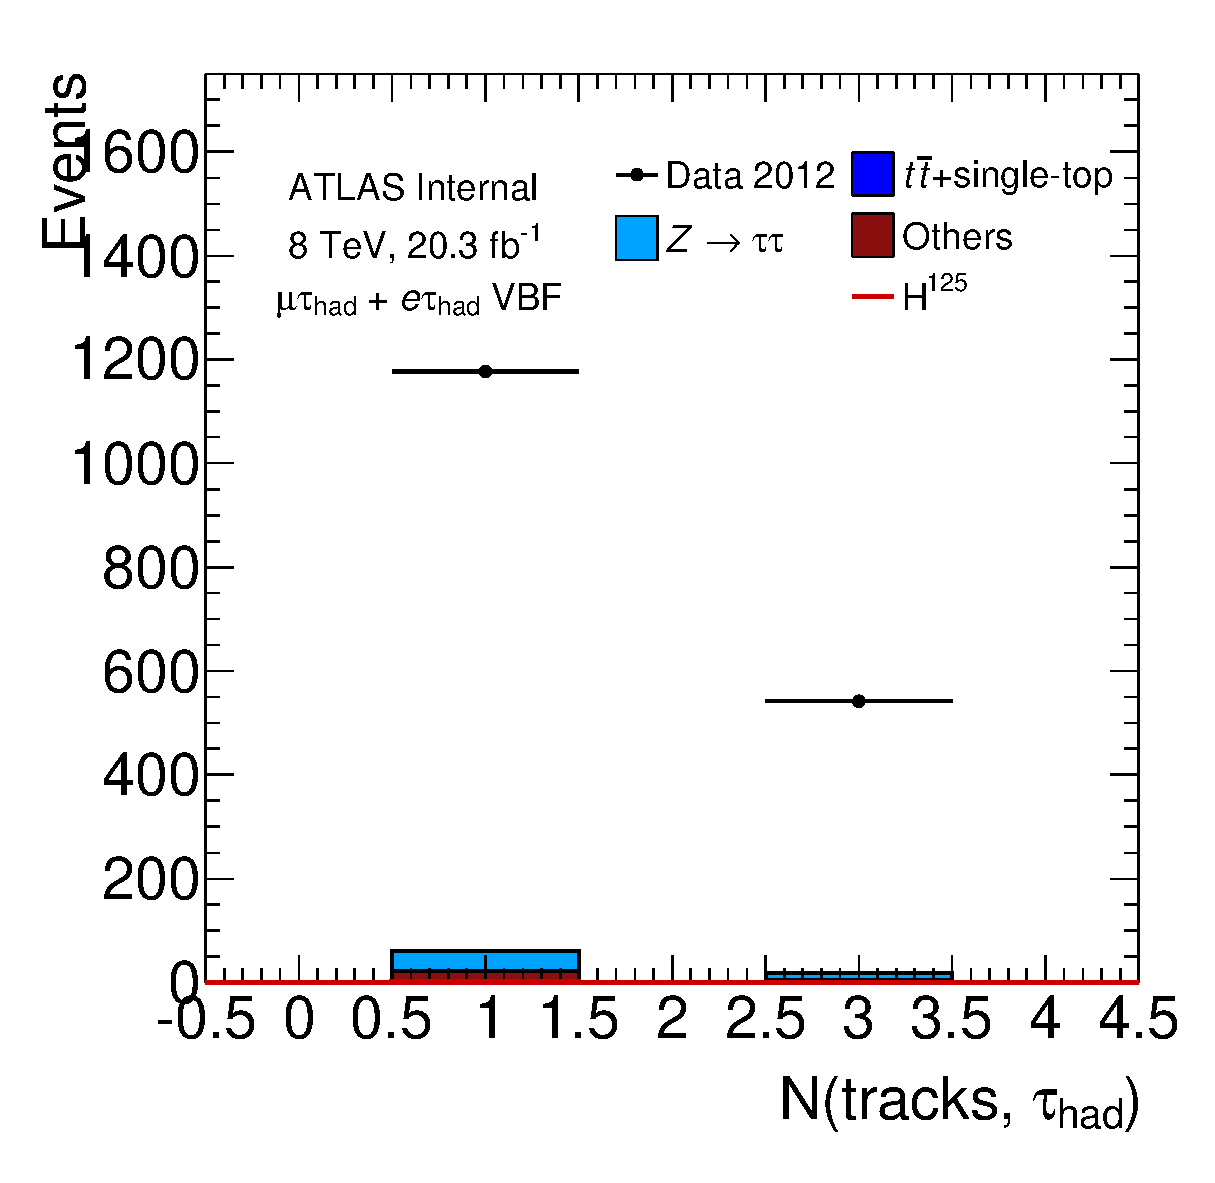
\includegraphics[width=0.32\textwidth]{figures/antitaus/tau-numTrack}
  % --------------
  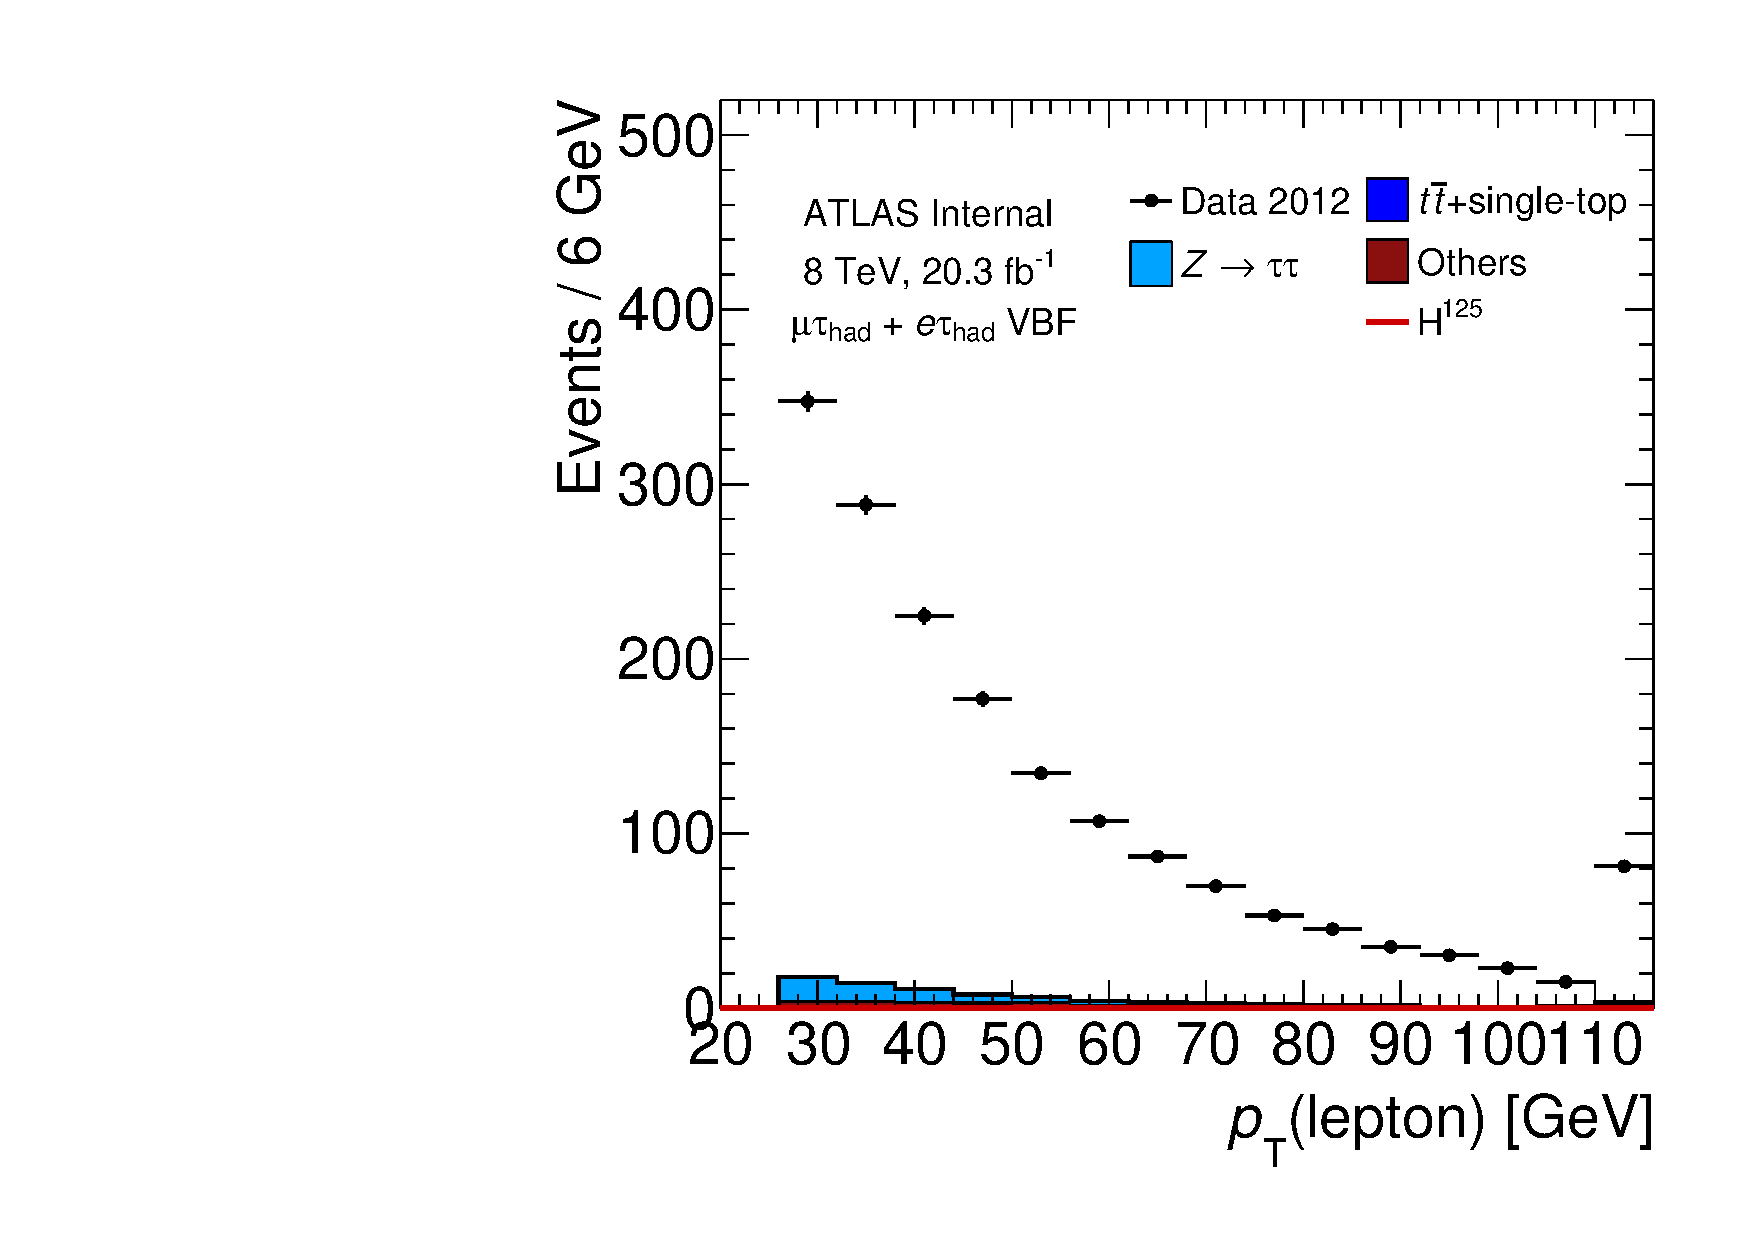
\includegraphics[width=0.32\textwidth]{figures/antitaus/lep-pt-hi}
  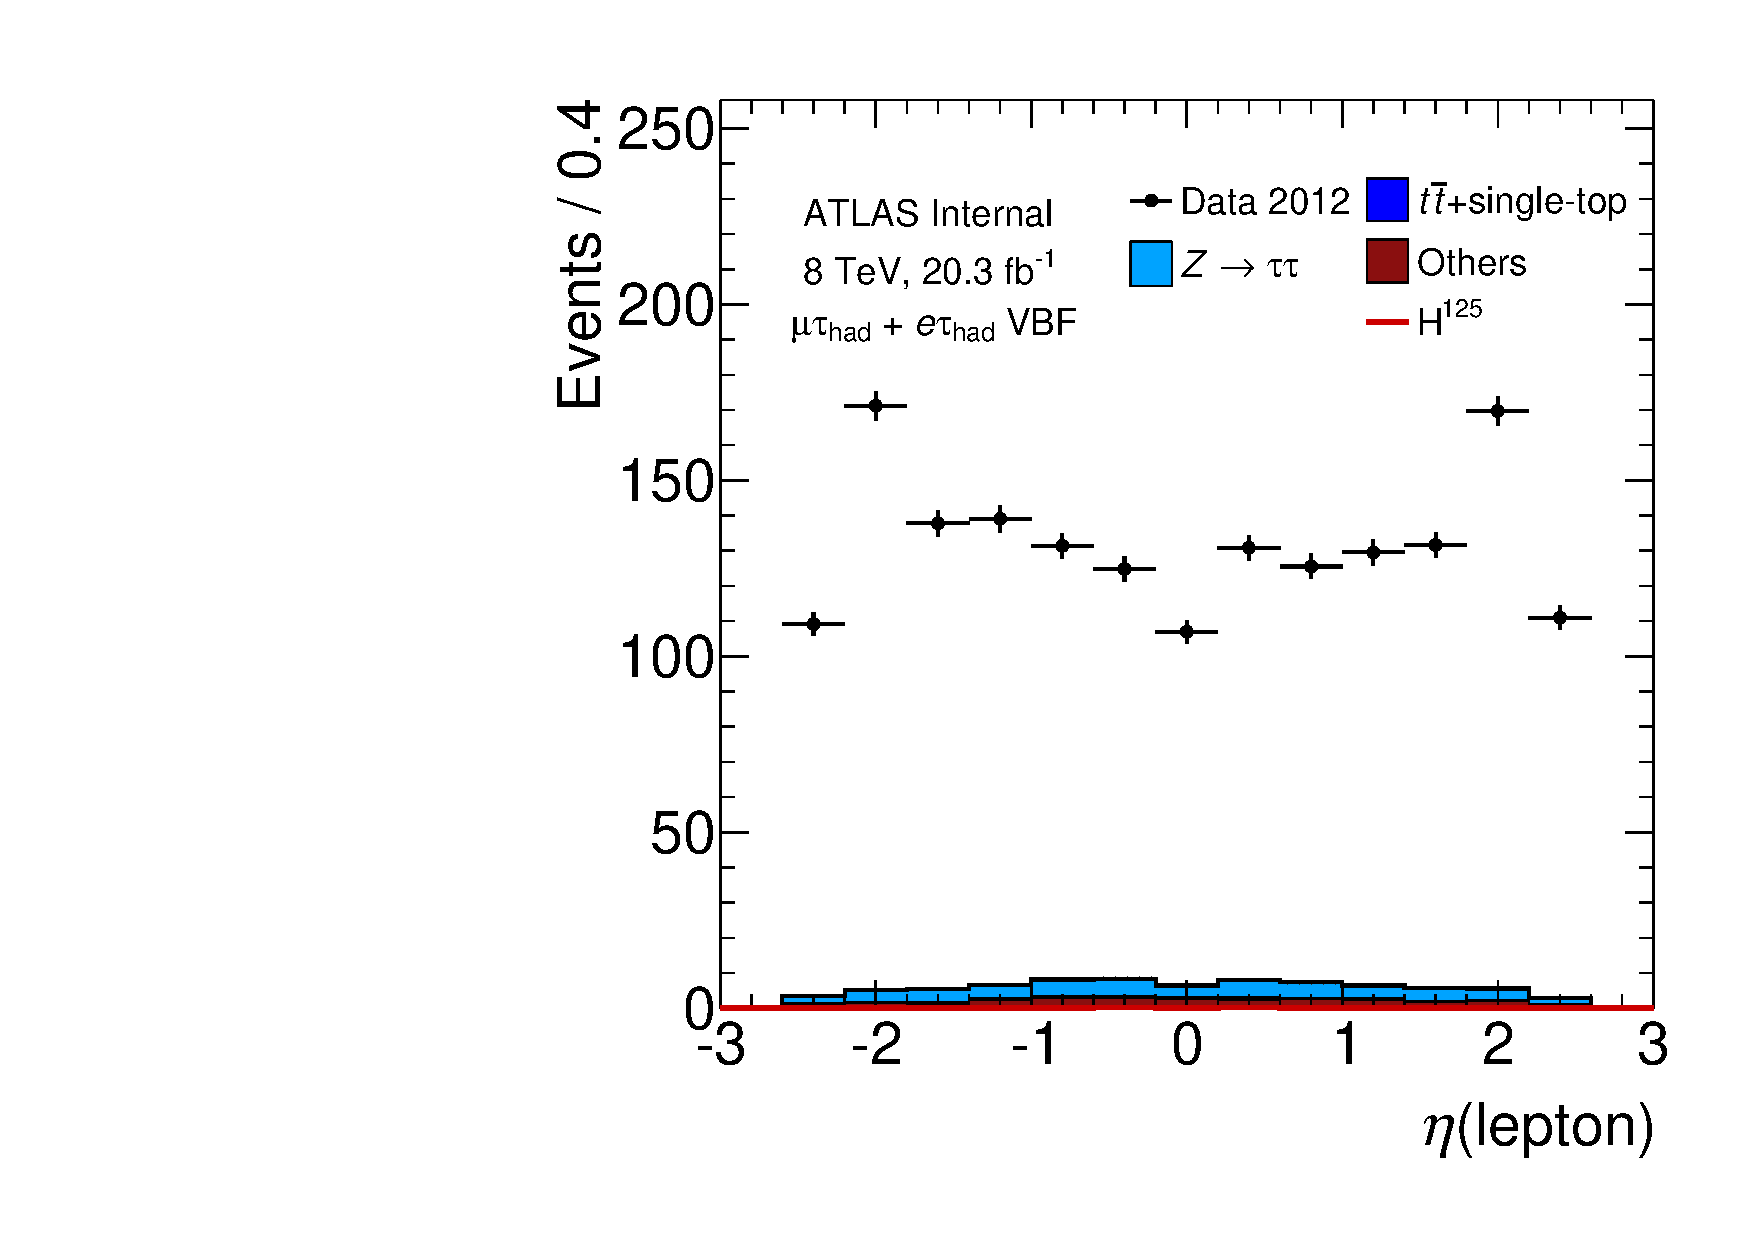
\includegraphics[width=0.32\textwidth]{figures/antitaus/lep-eta}
  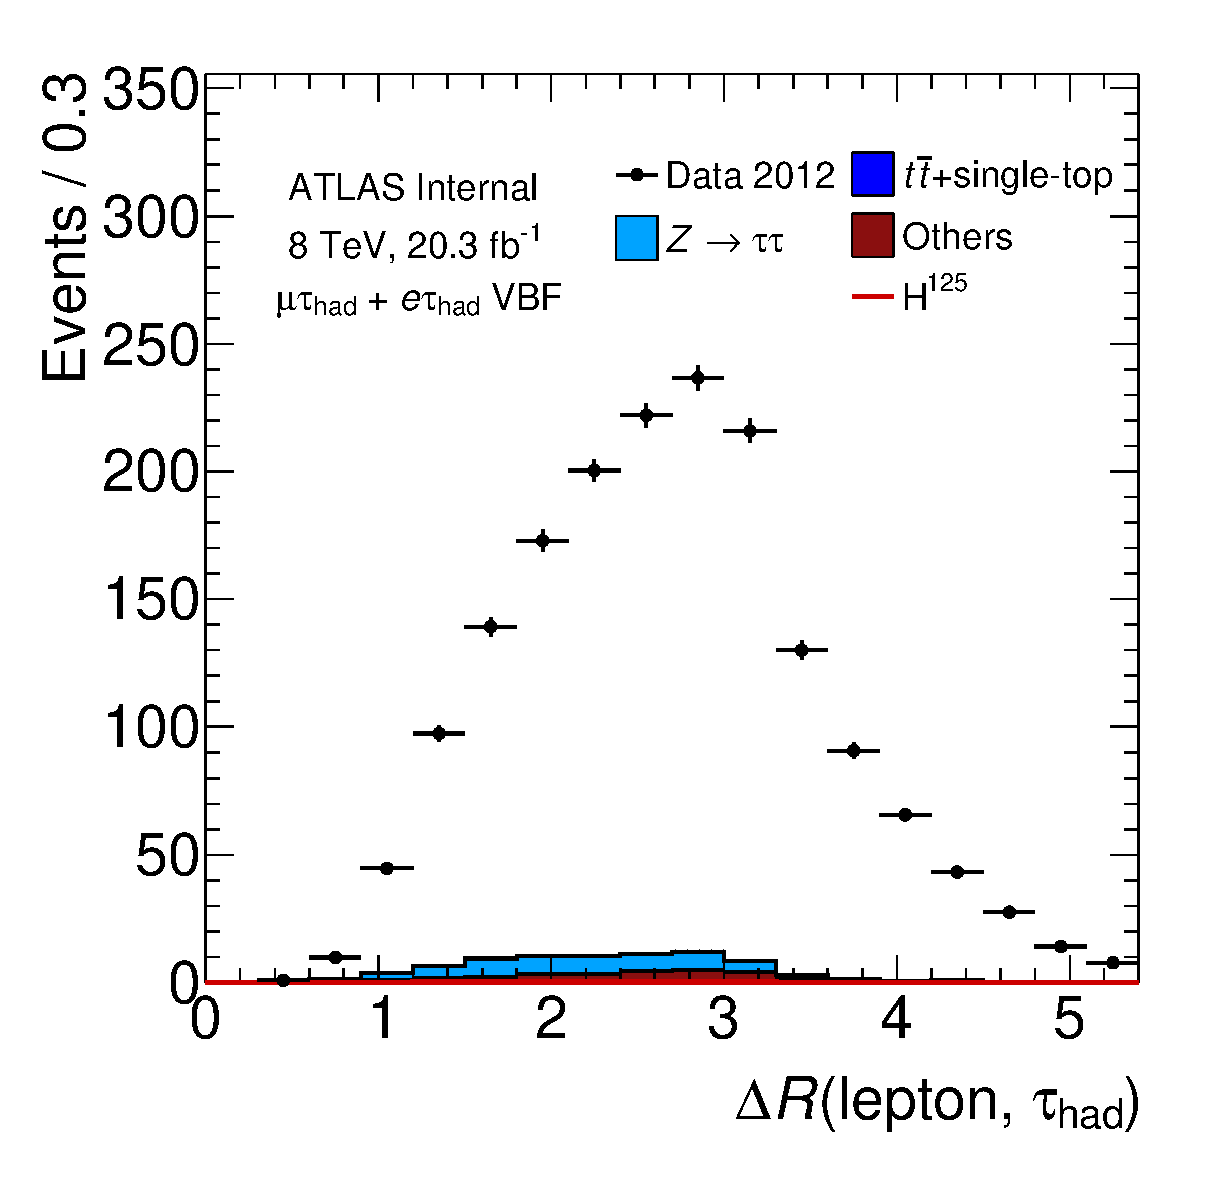
\includegraphics[width=0.32\textwidth]{figures/antitaus/taulep-dR}
  % --------------
  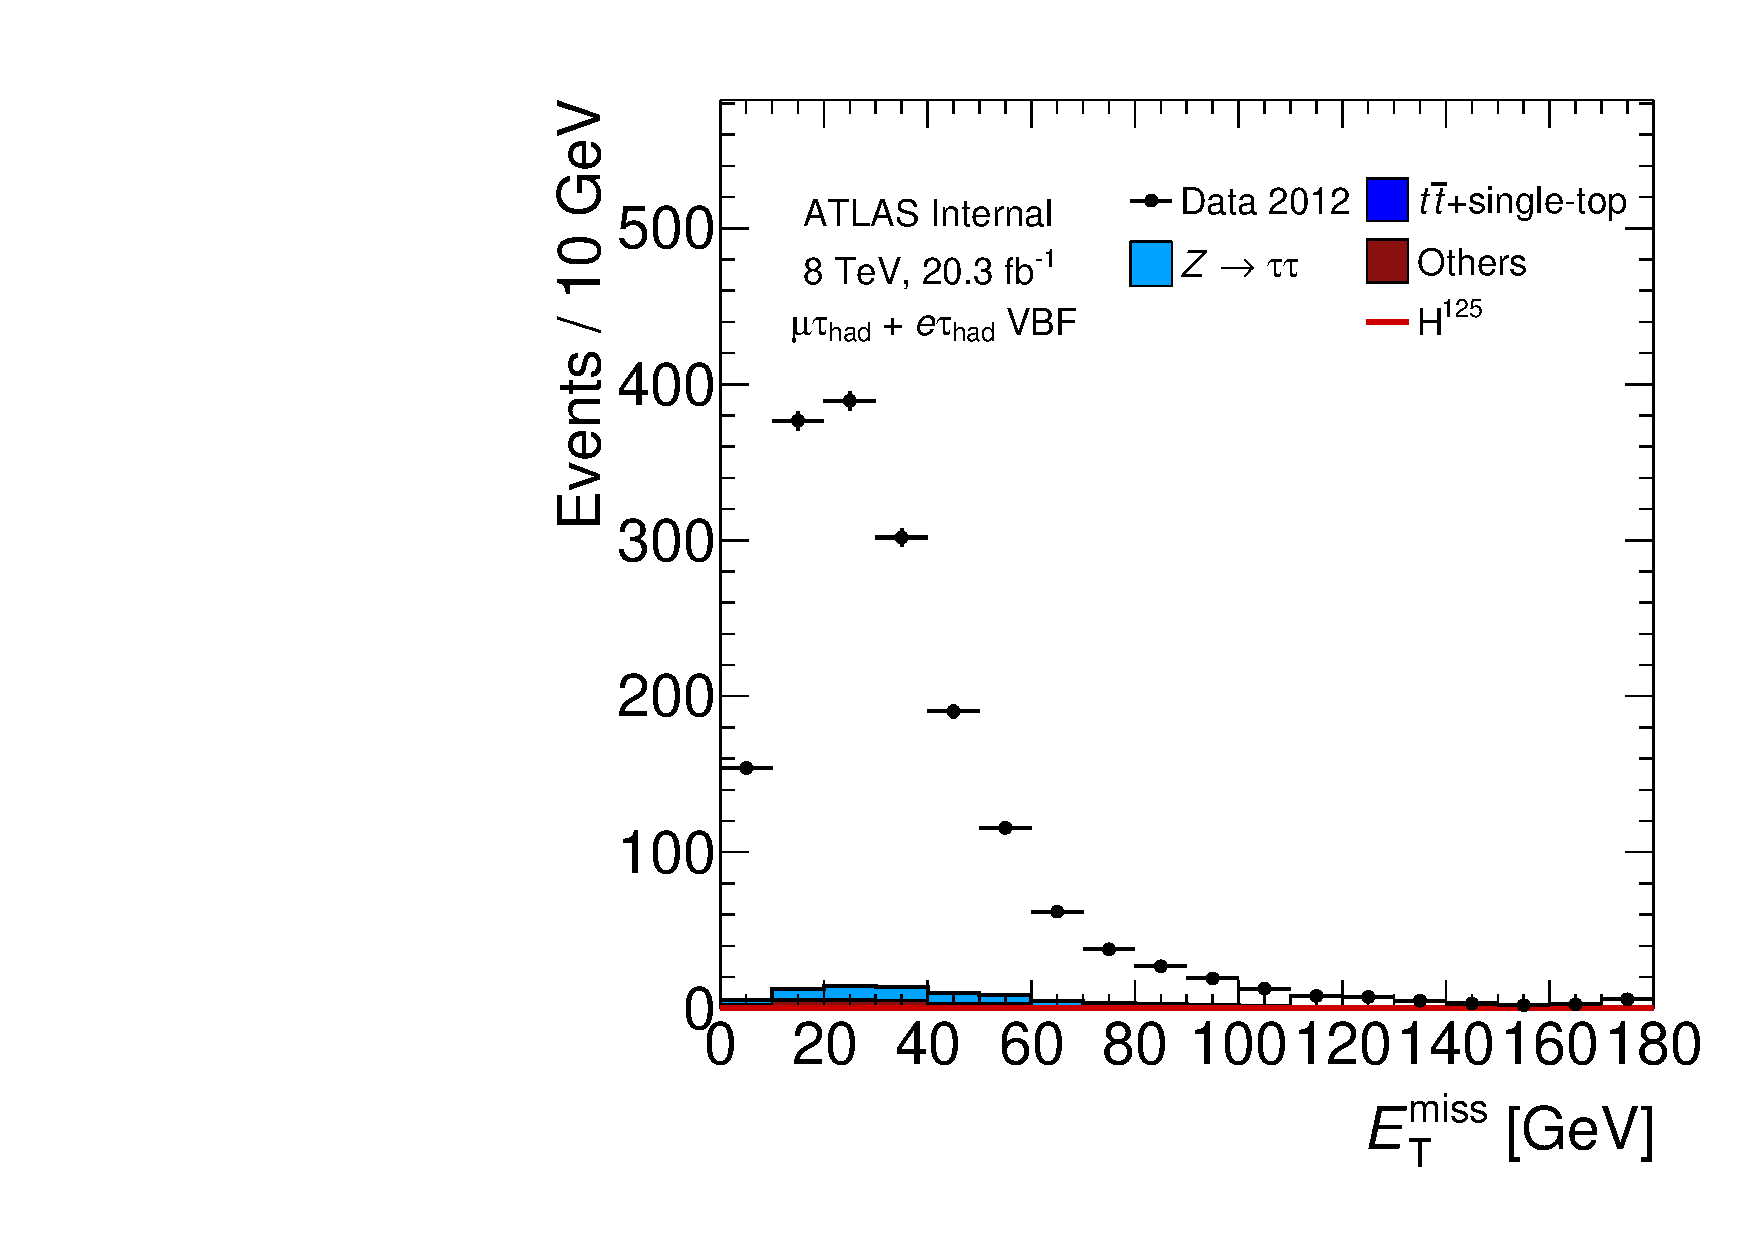
\includegraphics[width=0.32\textwidth]{figures/antitaus/met-pt-hi}
  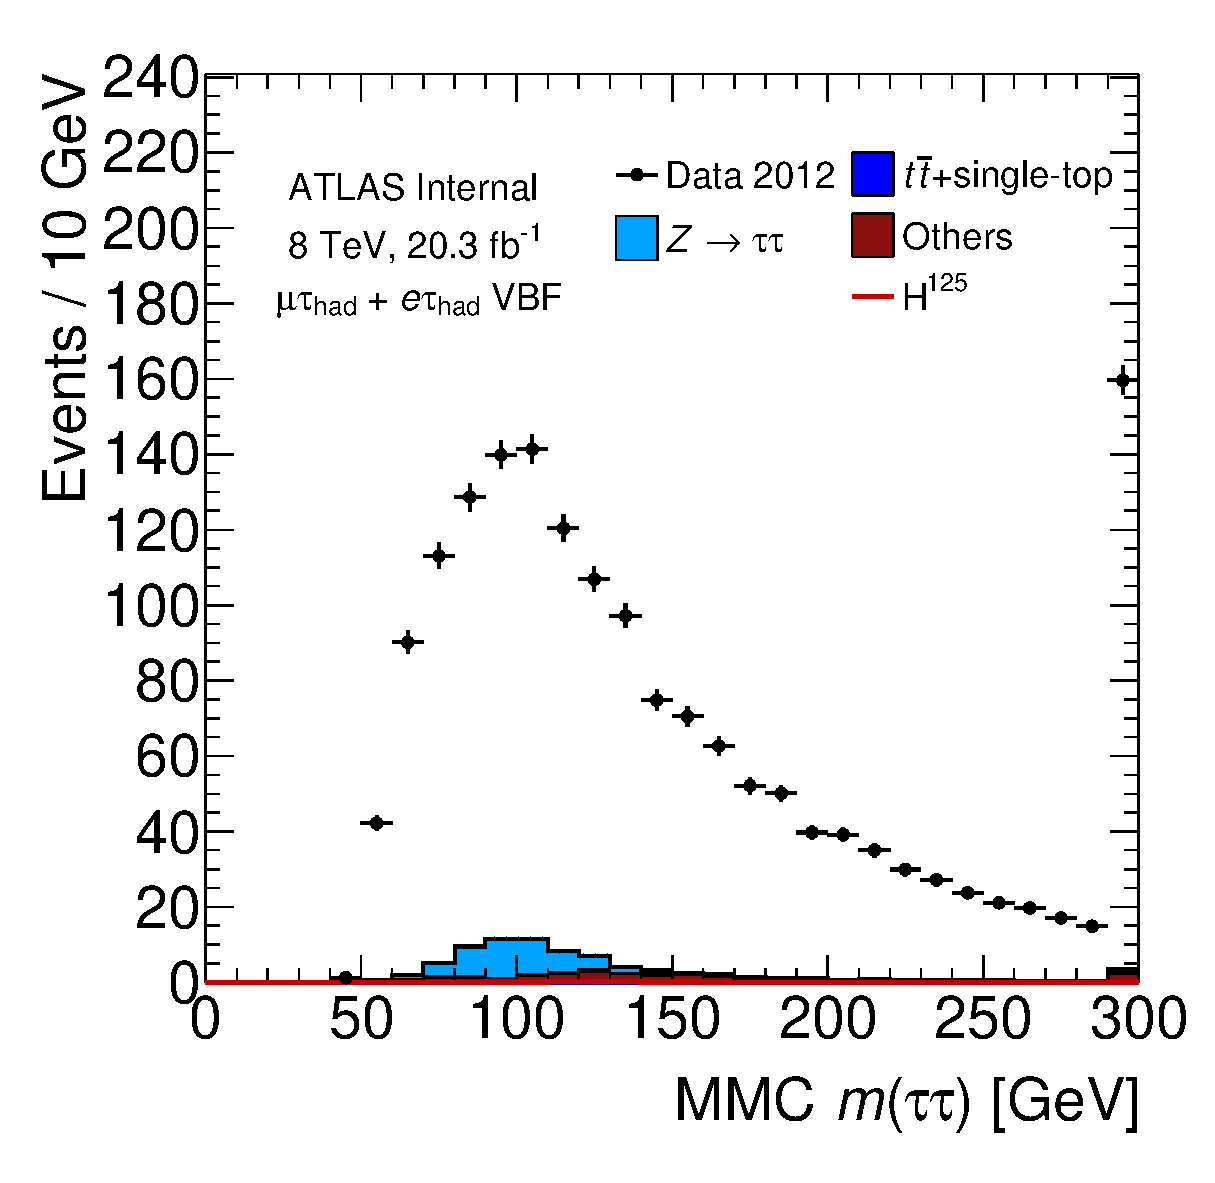
\includegraphics[width=0.32\textwidth]{figures/antitaus/mMMC}
  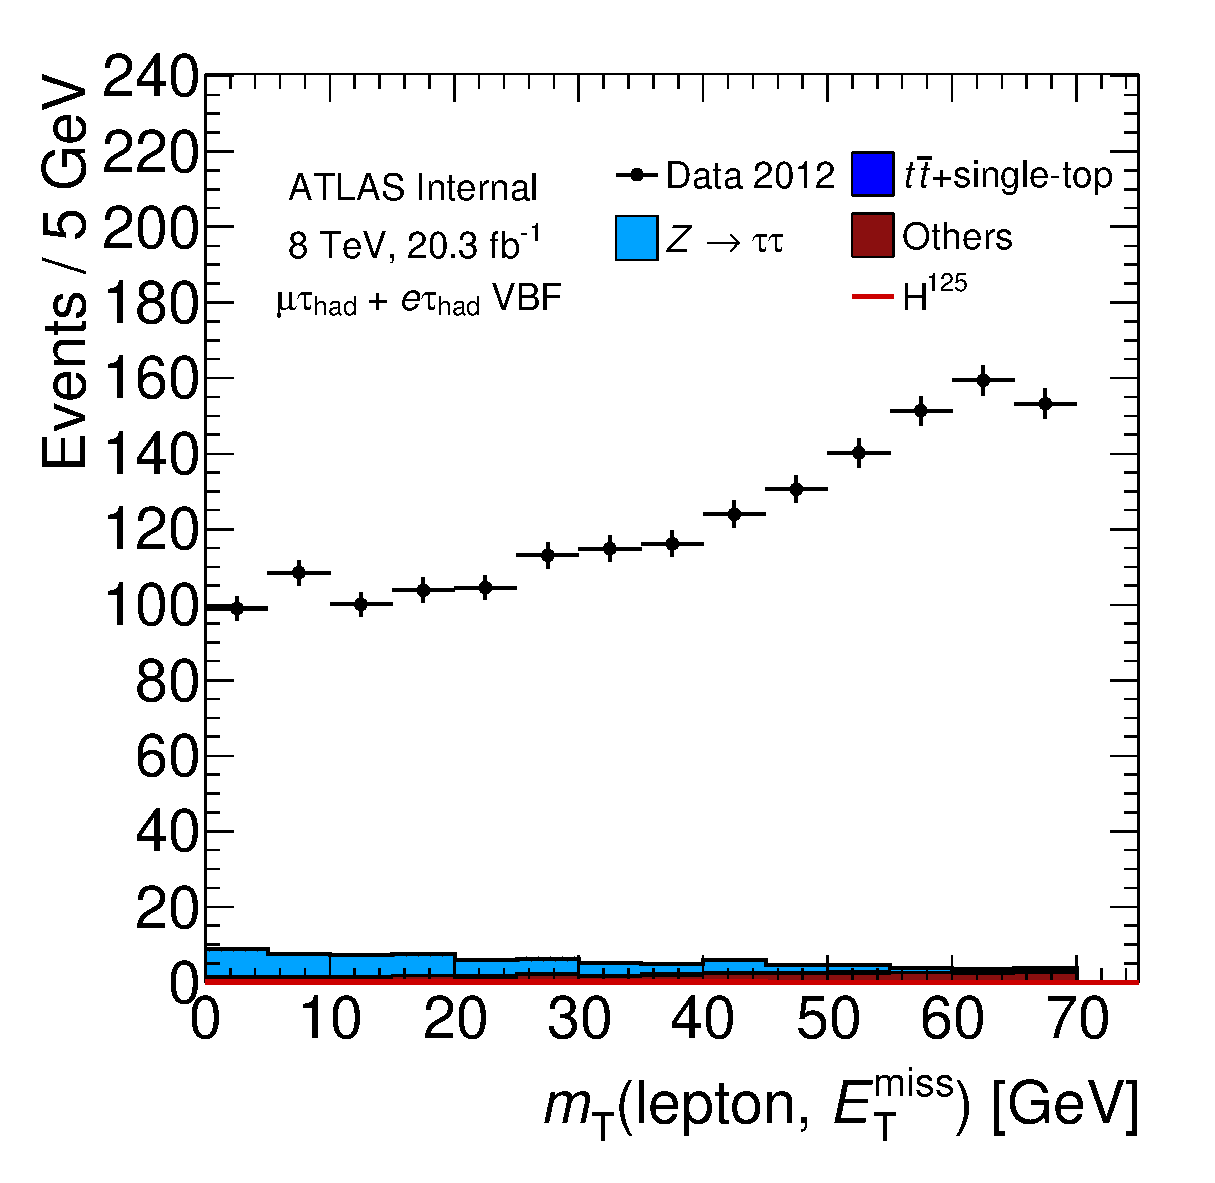
\includegraphics[width=0.32\textwidth]{figures/antitaus/mT}
  % --------------
  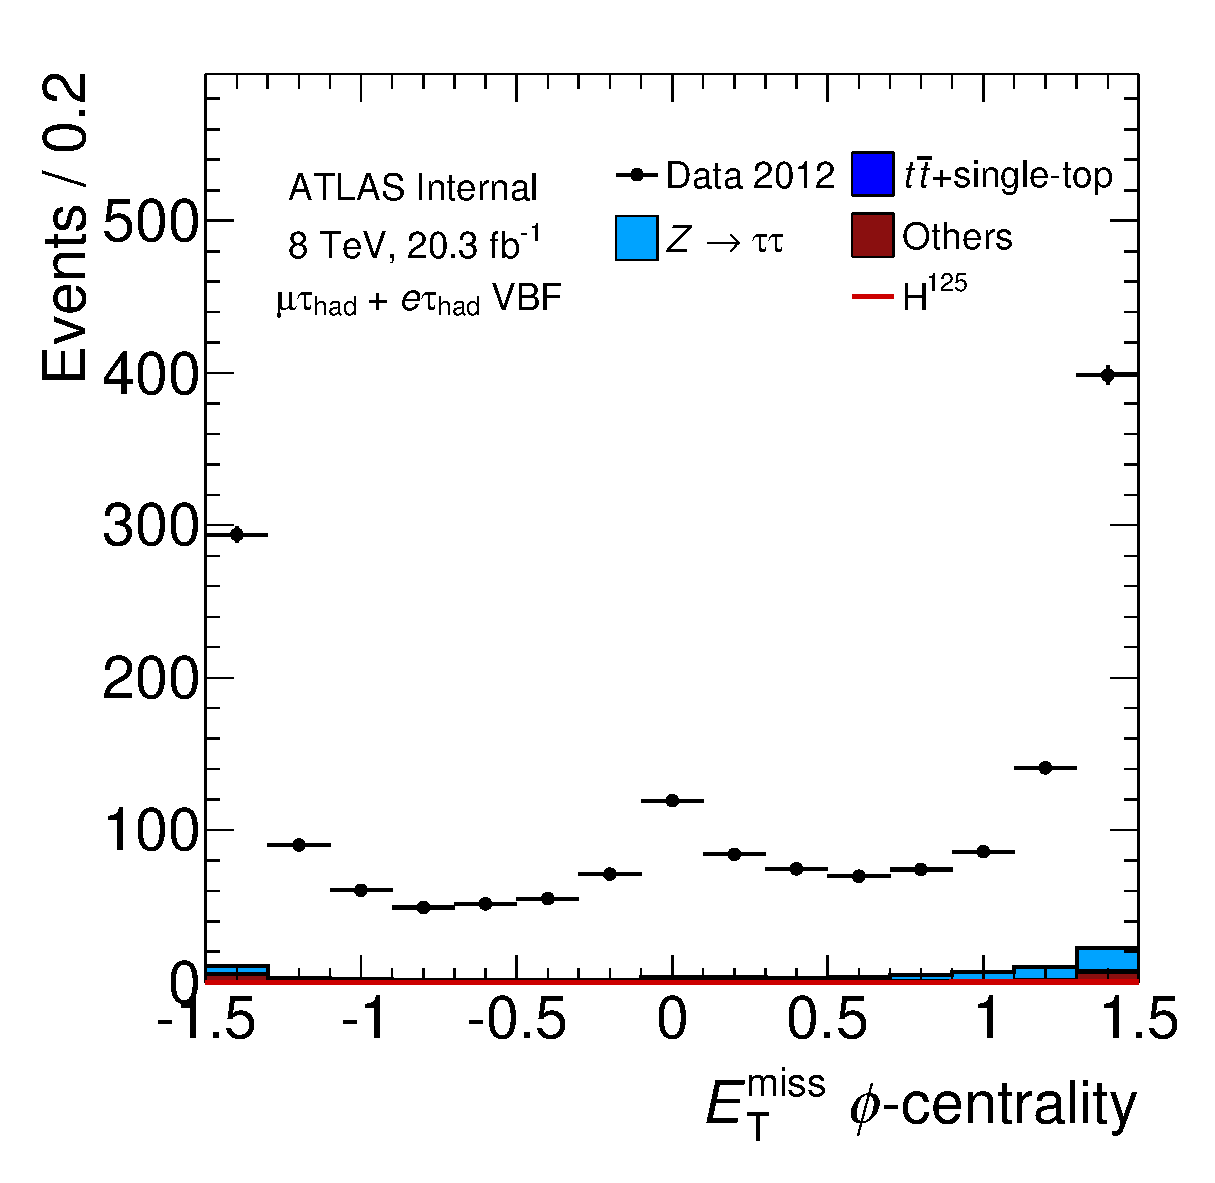
\includegraphics[width=0.32\textwidth]{figures/antitaus/met-phi-centrality}
  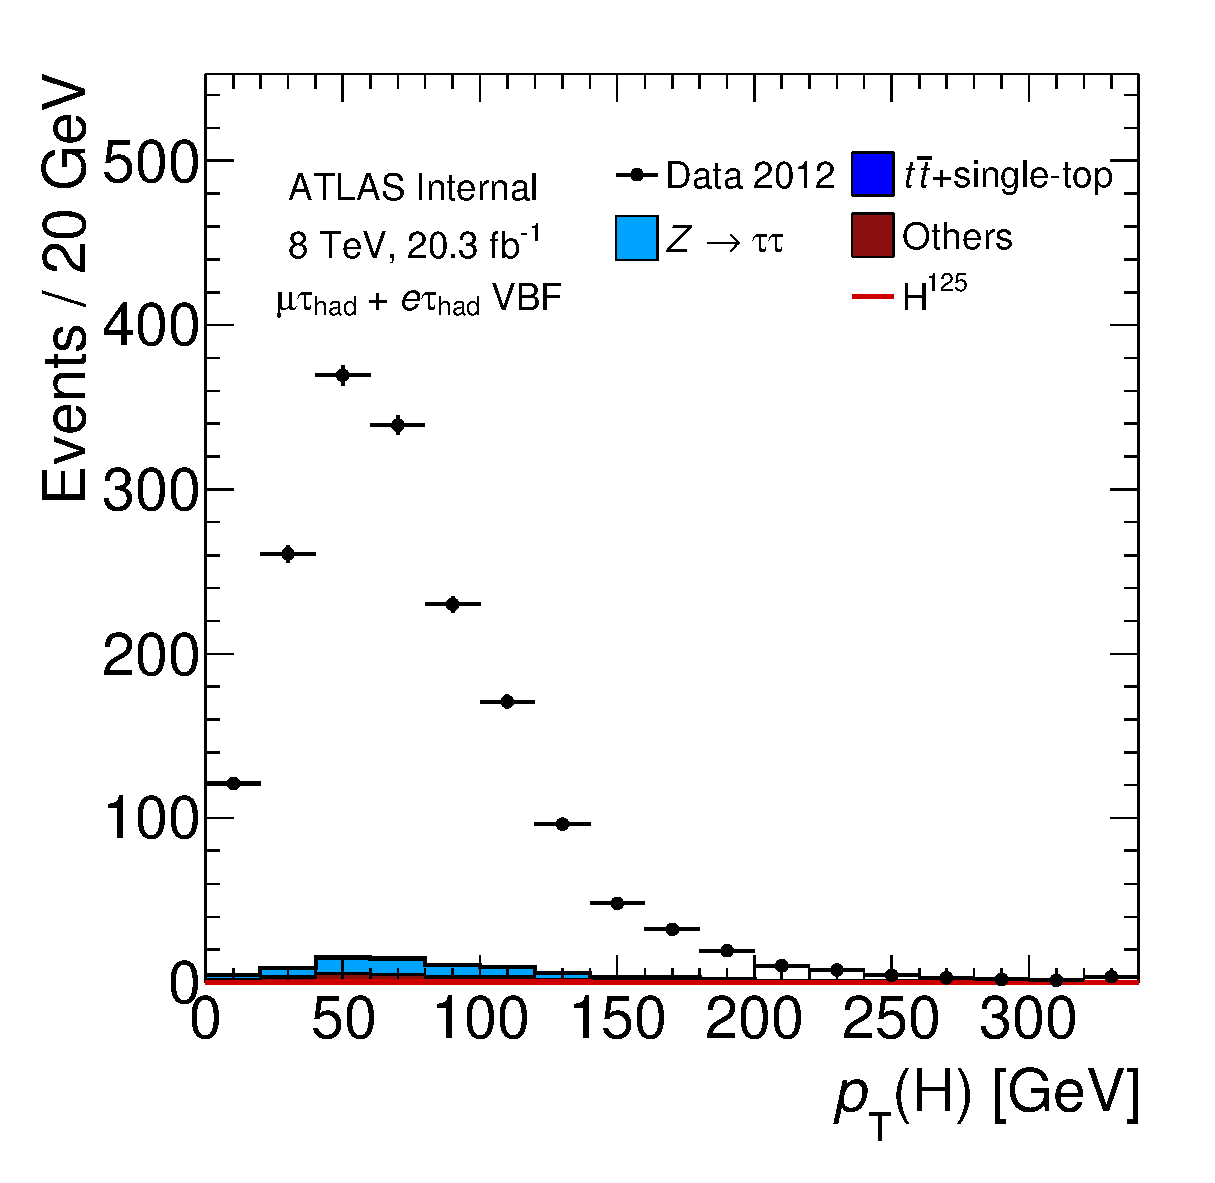
\includegraphics[width=0.32\textwidth]{figures/antitaus/H-pt-hi}
  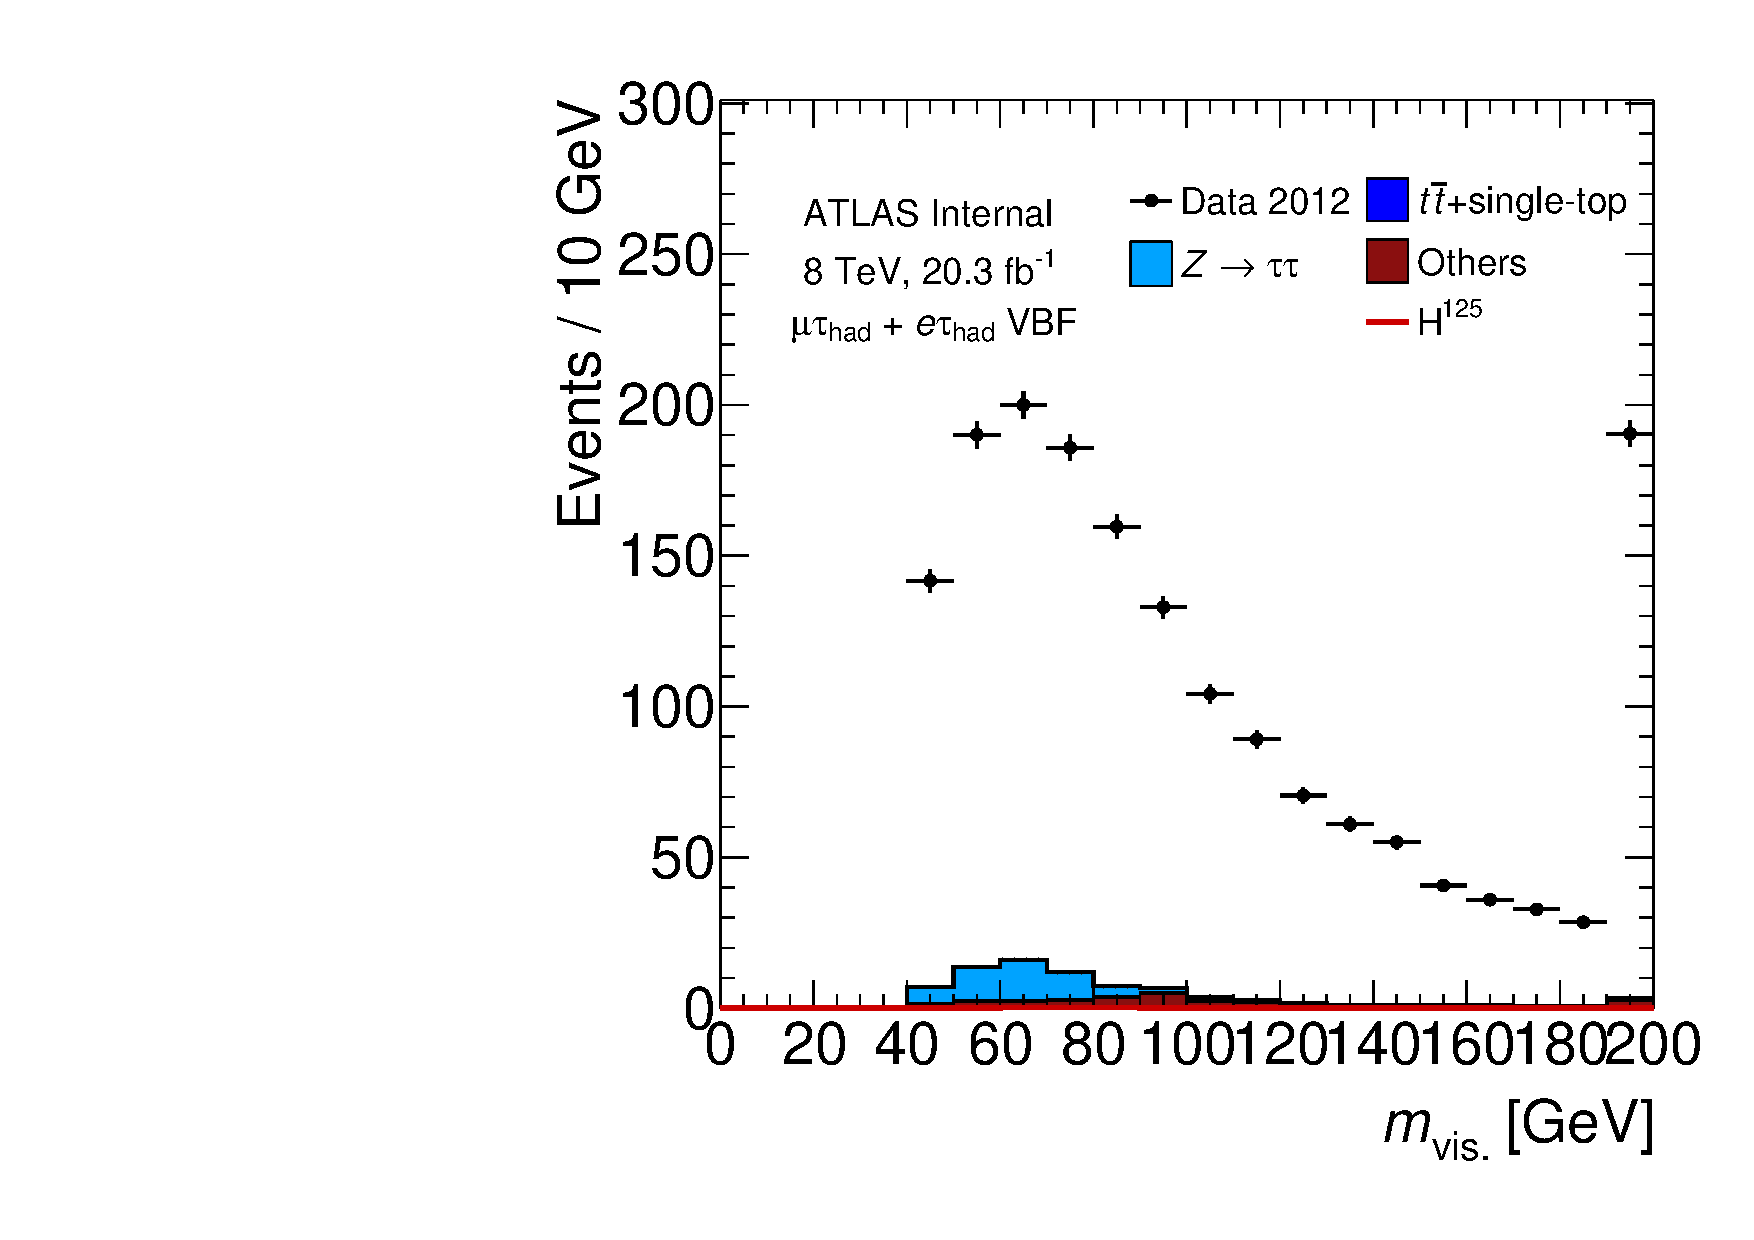
\includegraphics[width=0.32\textwidth]{figures/antitaus/mvis}
  \caption{Data events in the VBF category which fail $\tauh$ identification but fulfill all other requirements. The contamination of $\Ztautaulh$ and other processes without $\fakes$ is less than 10\%.}
  \label{fig:backgrounds-antitaus-taus}
\end{figure}

\clearpage

\begin{figure}[tp]
  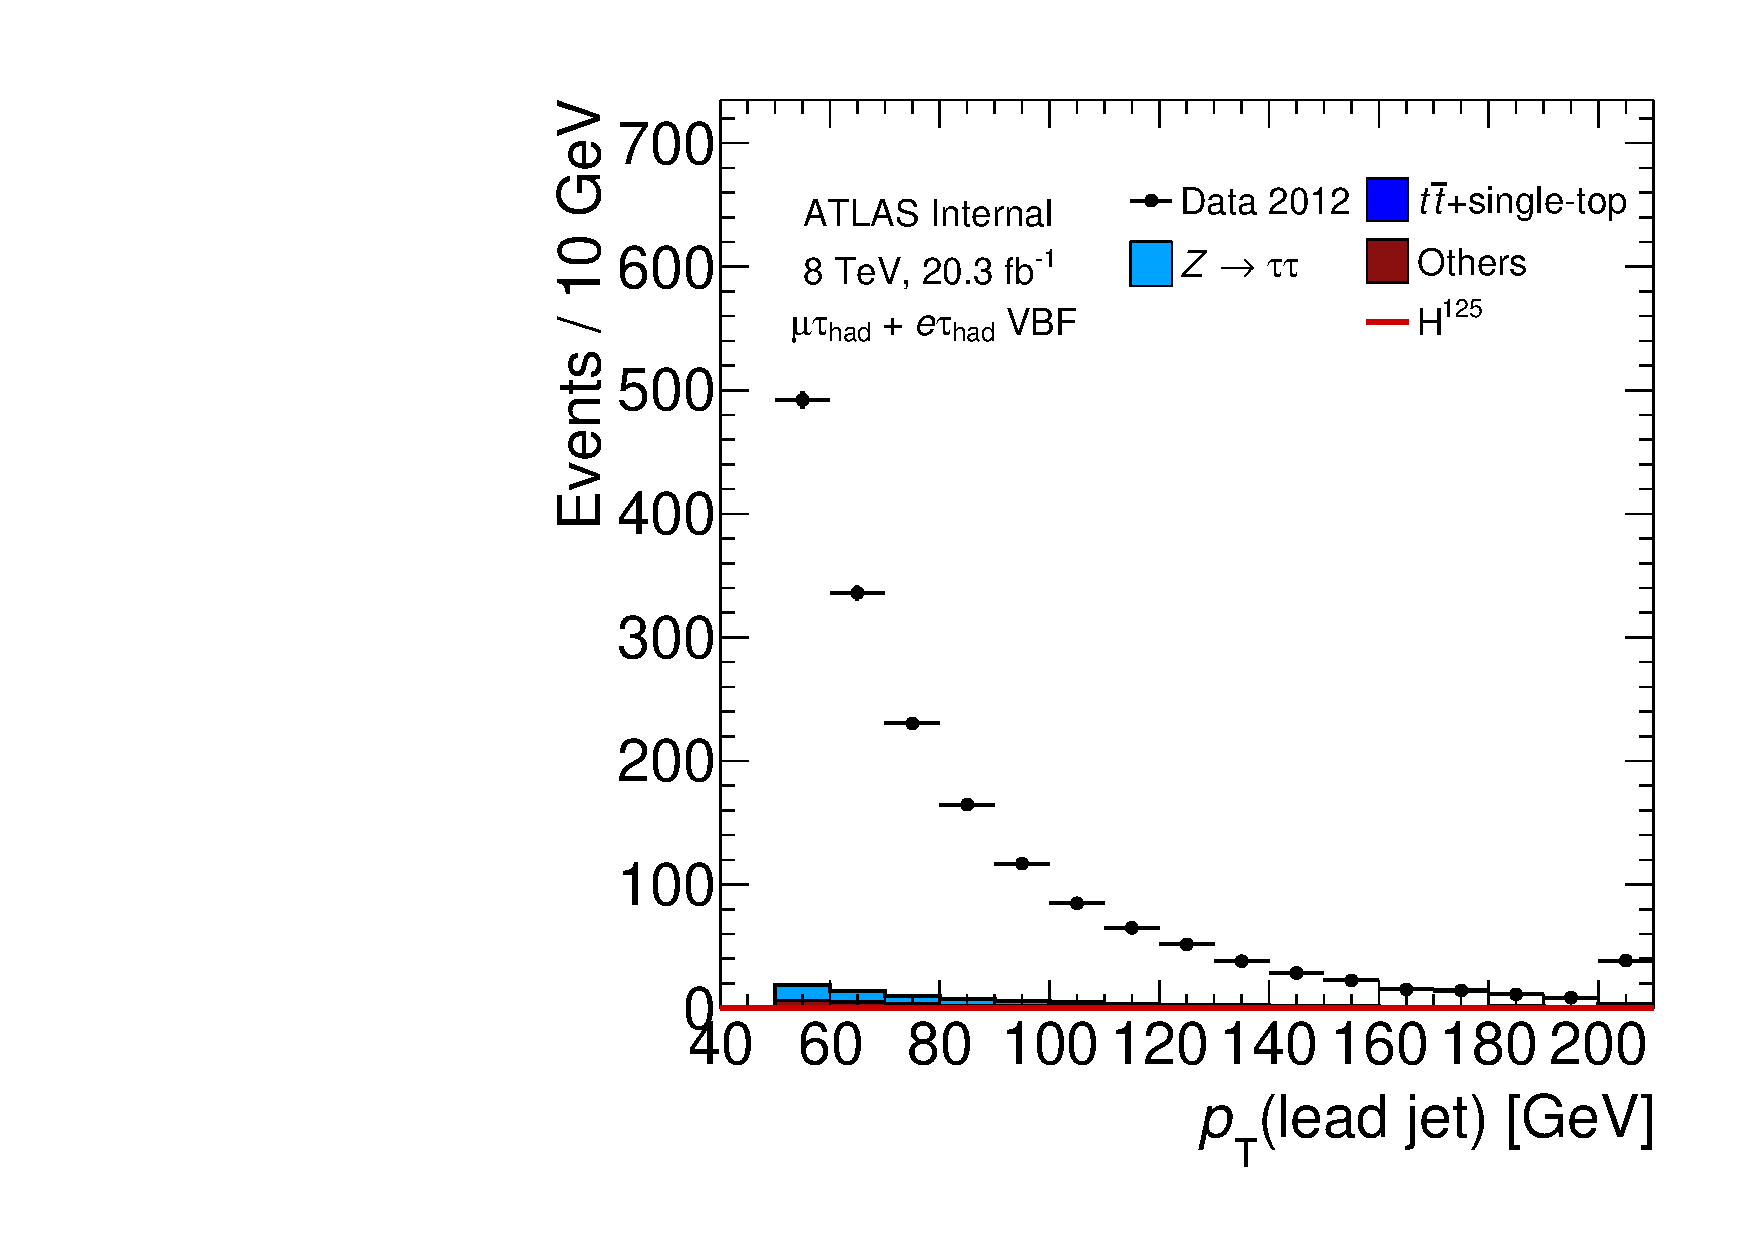
\includegraphics[width=0.32\textwidth]{figures/antitaus/jet-1-pt}
  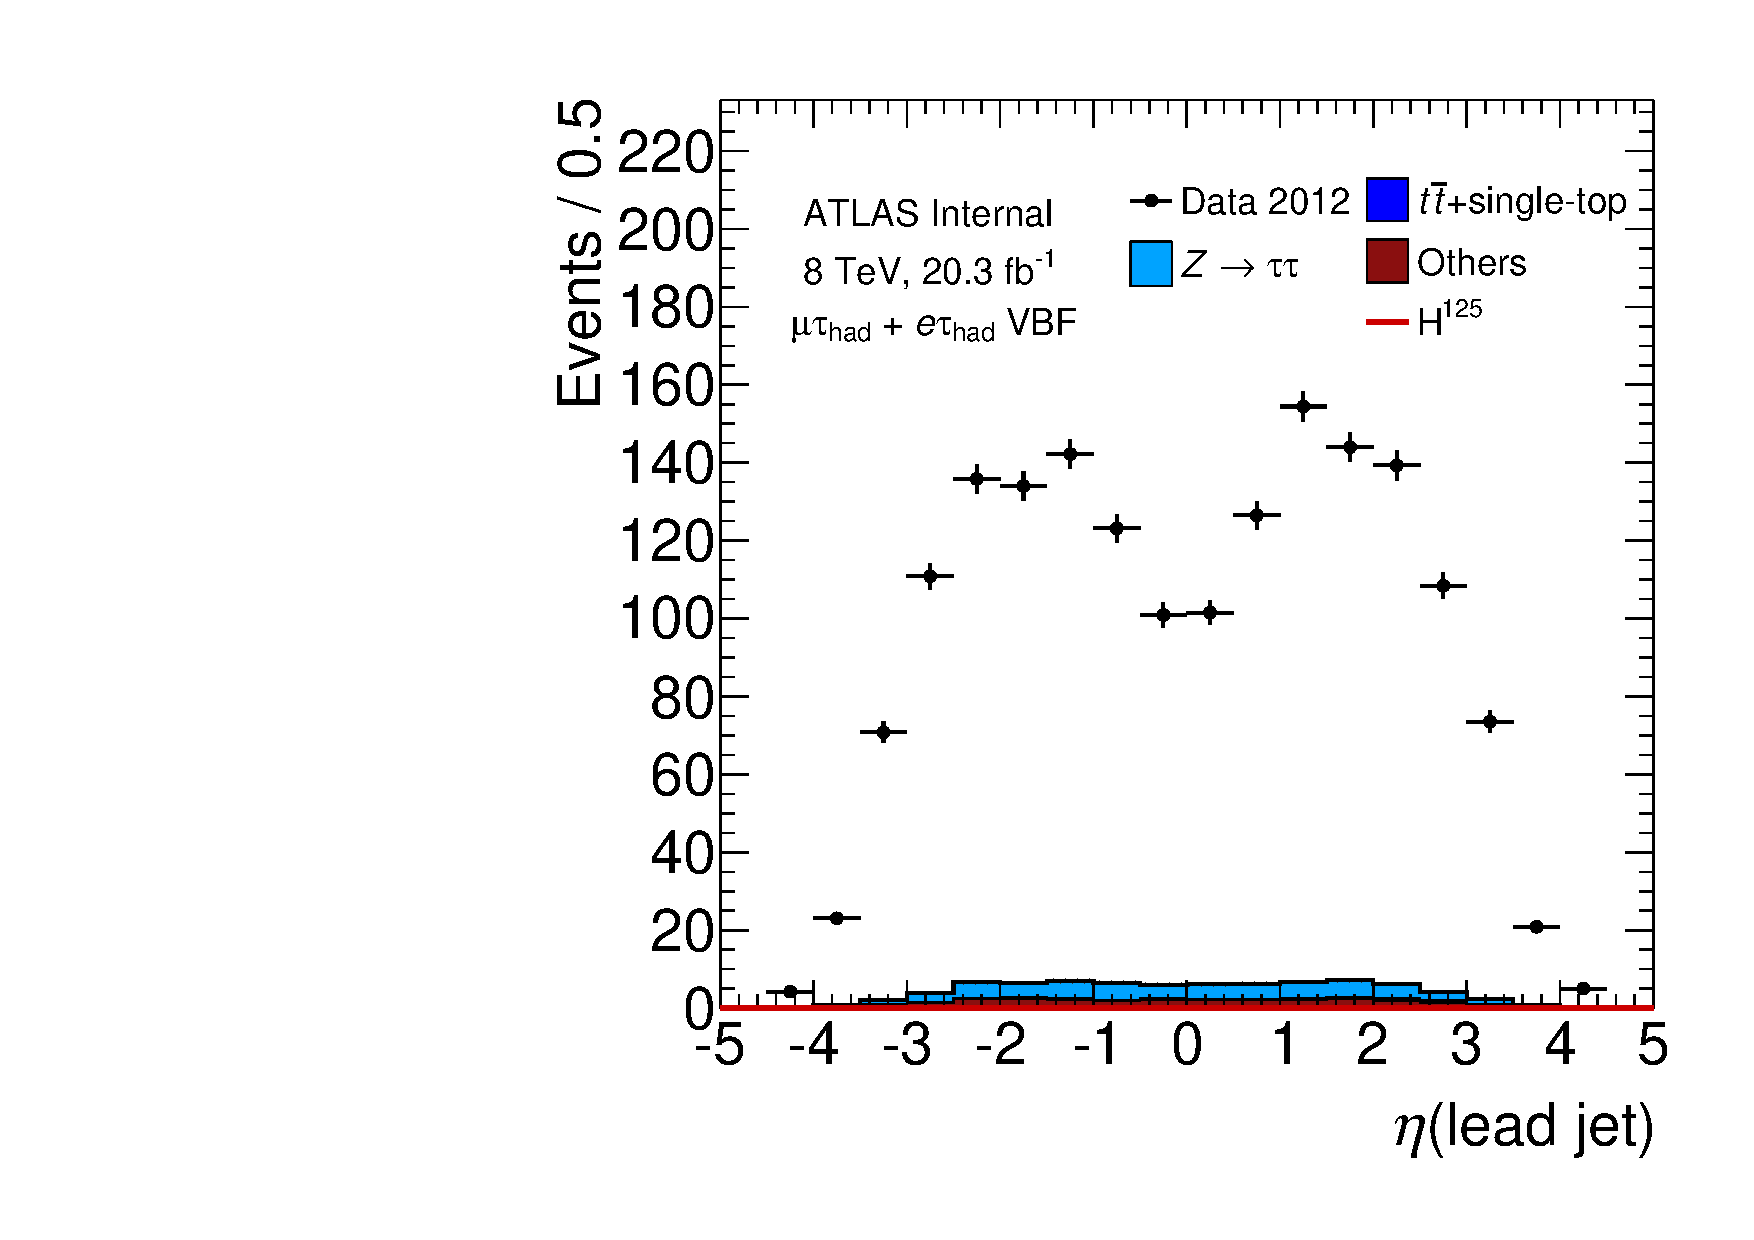
\includegraphics[width=0.32\textwidth]{figures/antitaus/jet-1-eta}
  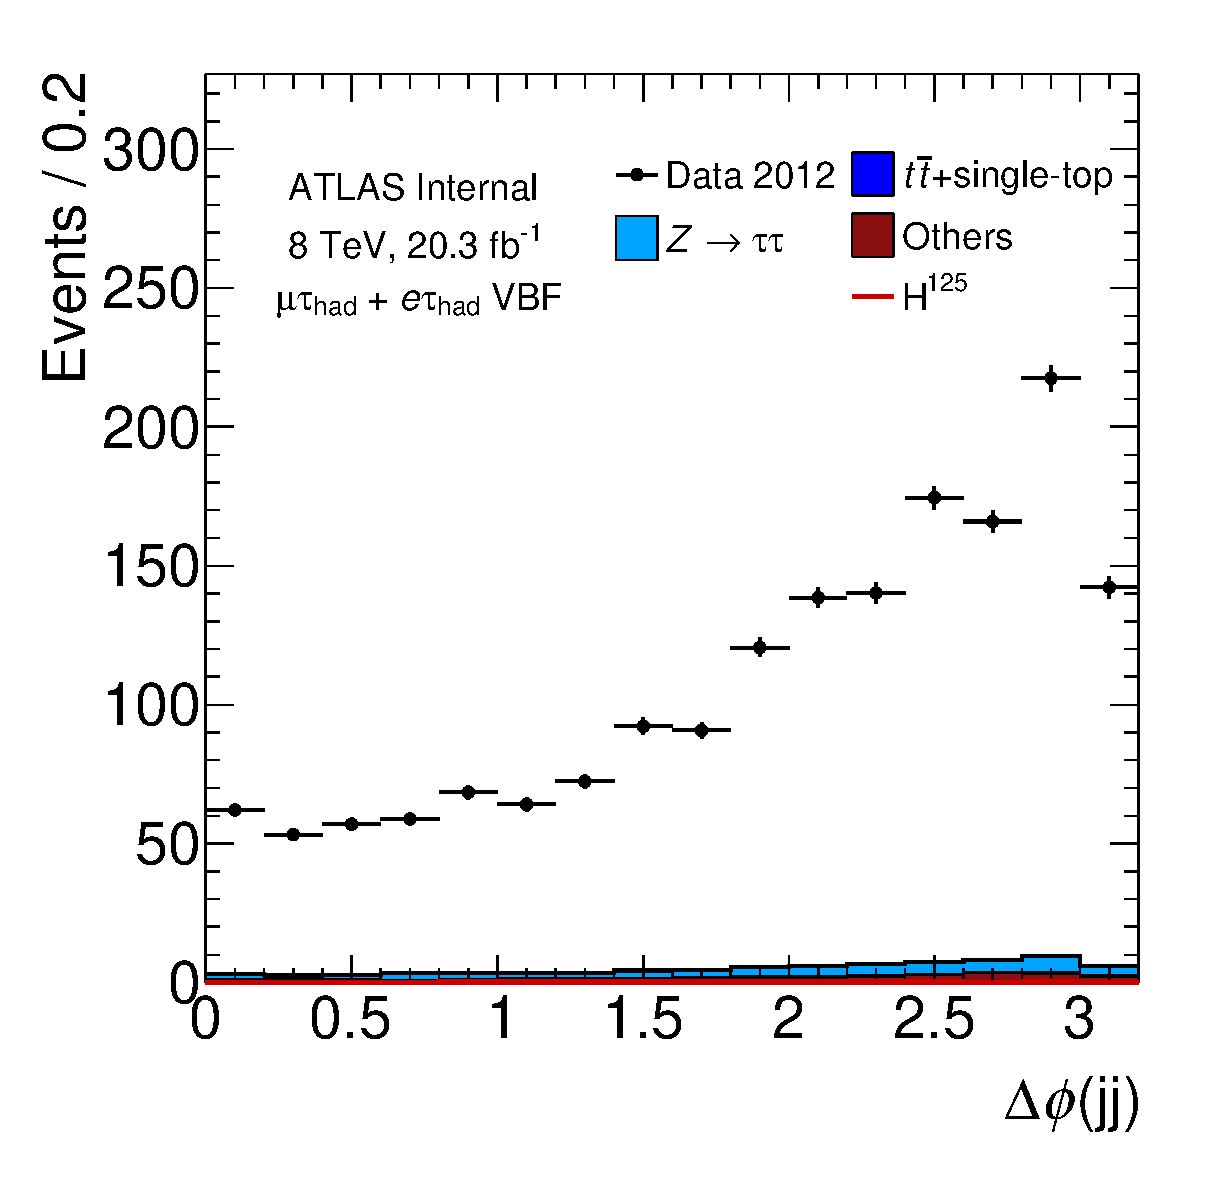
\includegraphics[width=0.32\textwidth]{figures/antitaus/jets-dphi}
  % --------------
  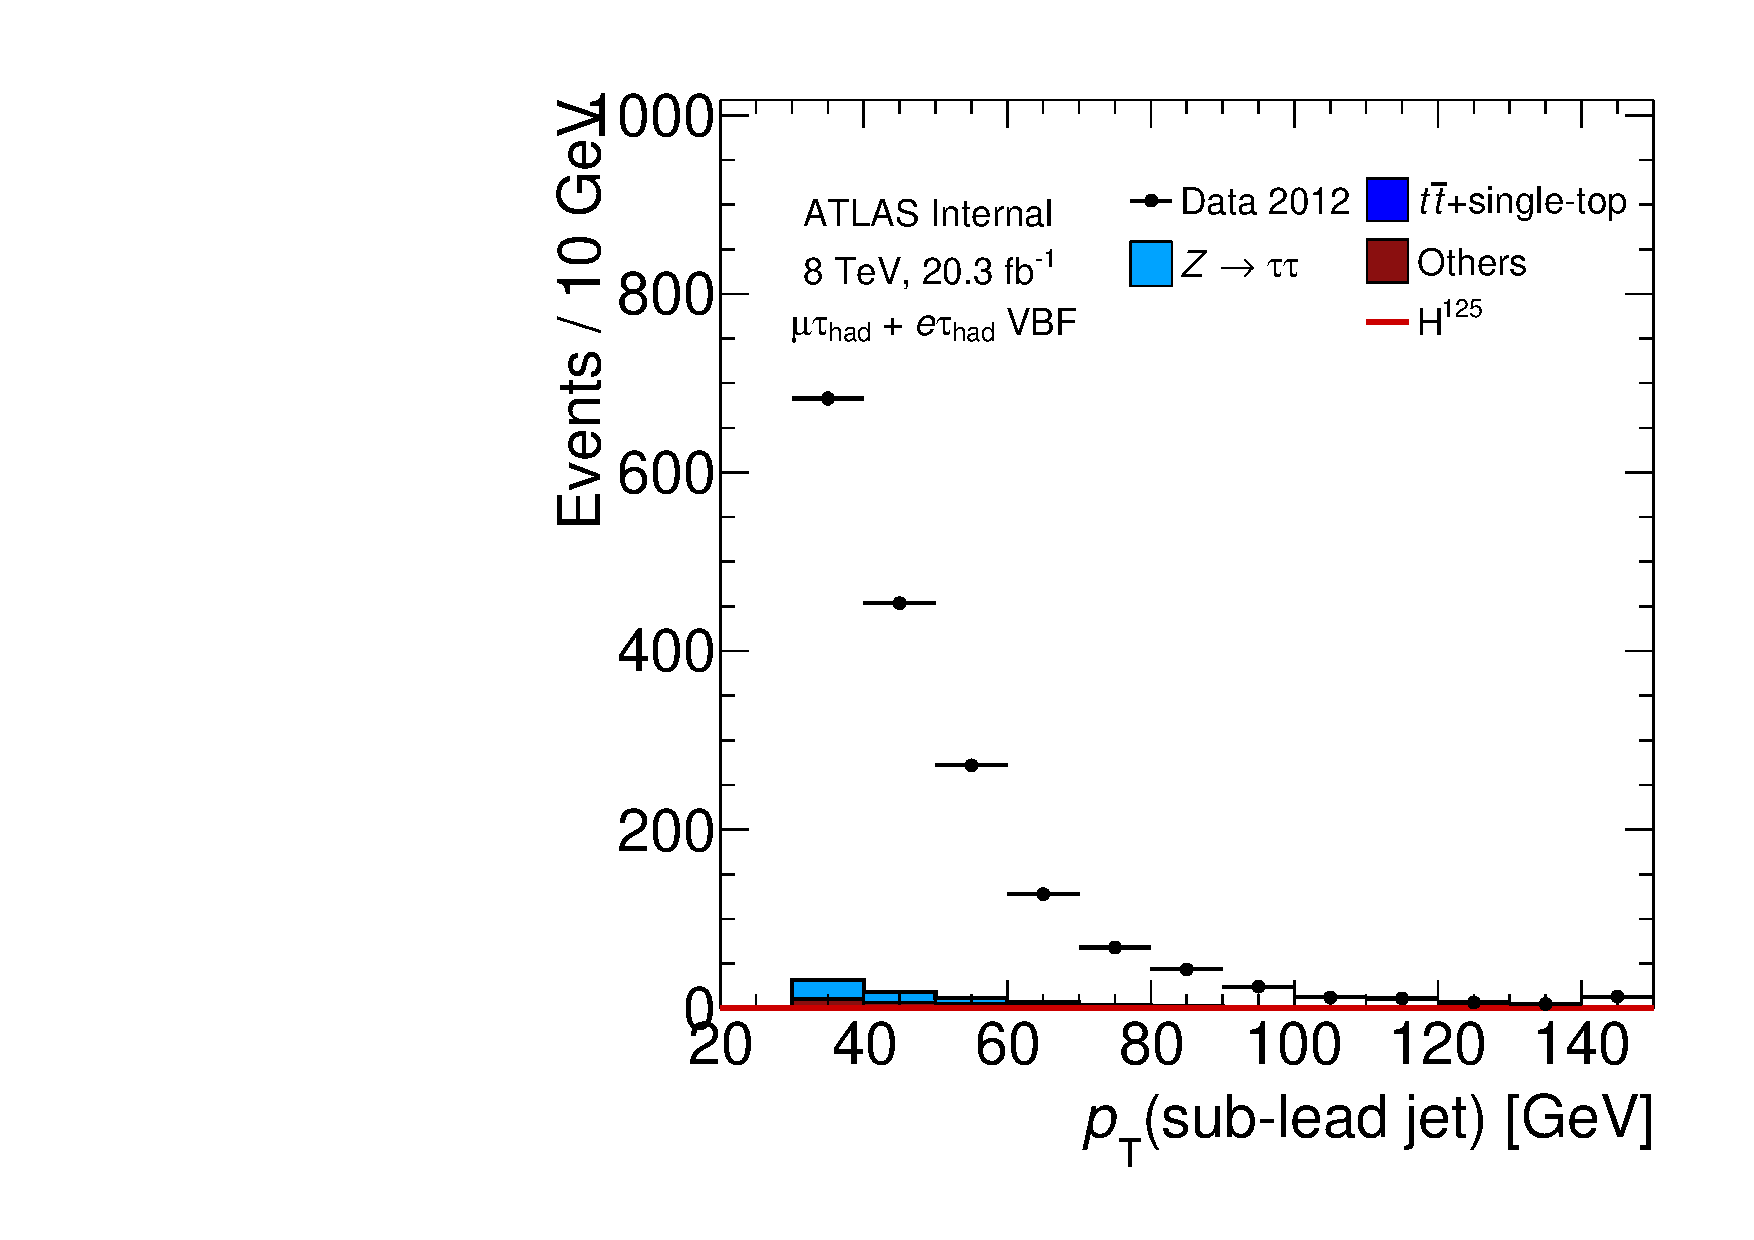
\includegraphics[width=0.32\textwidth]{figures/antitaus/jet-2-pt}
  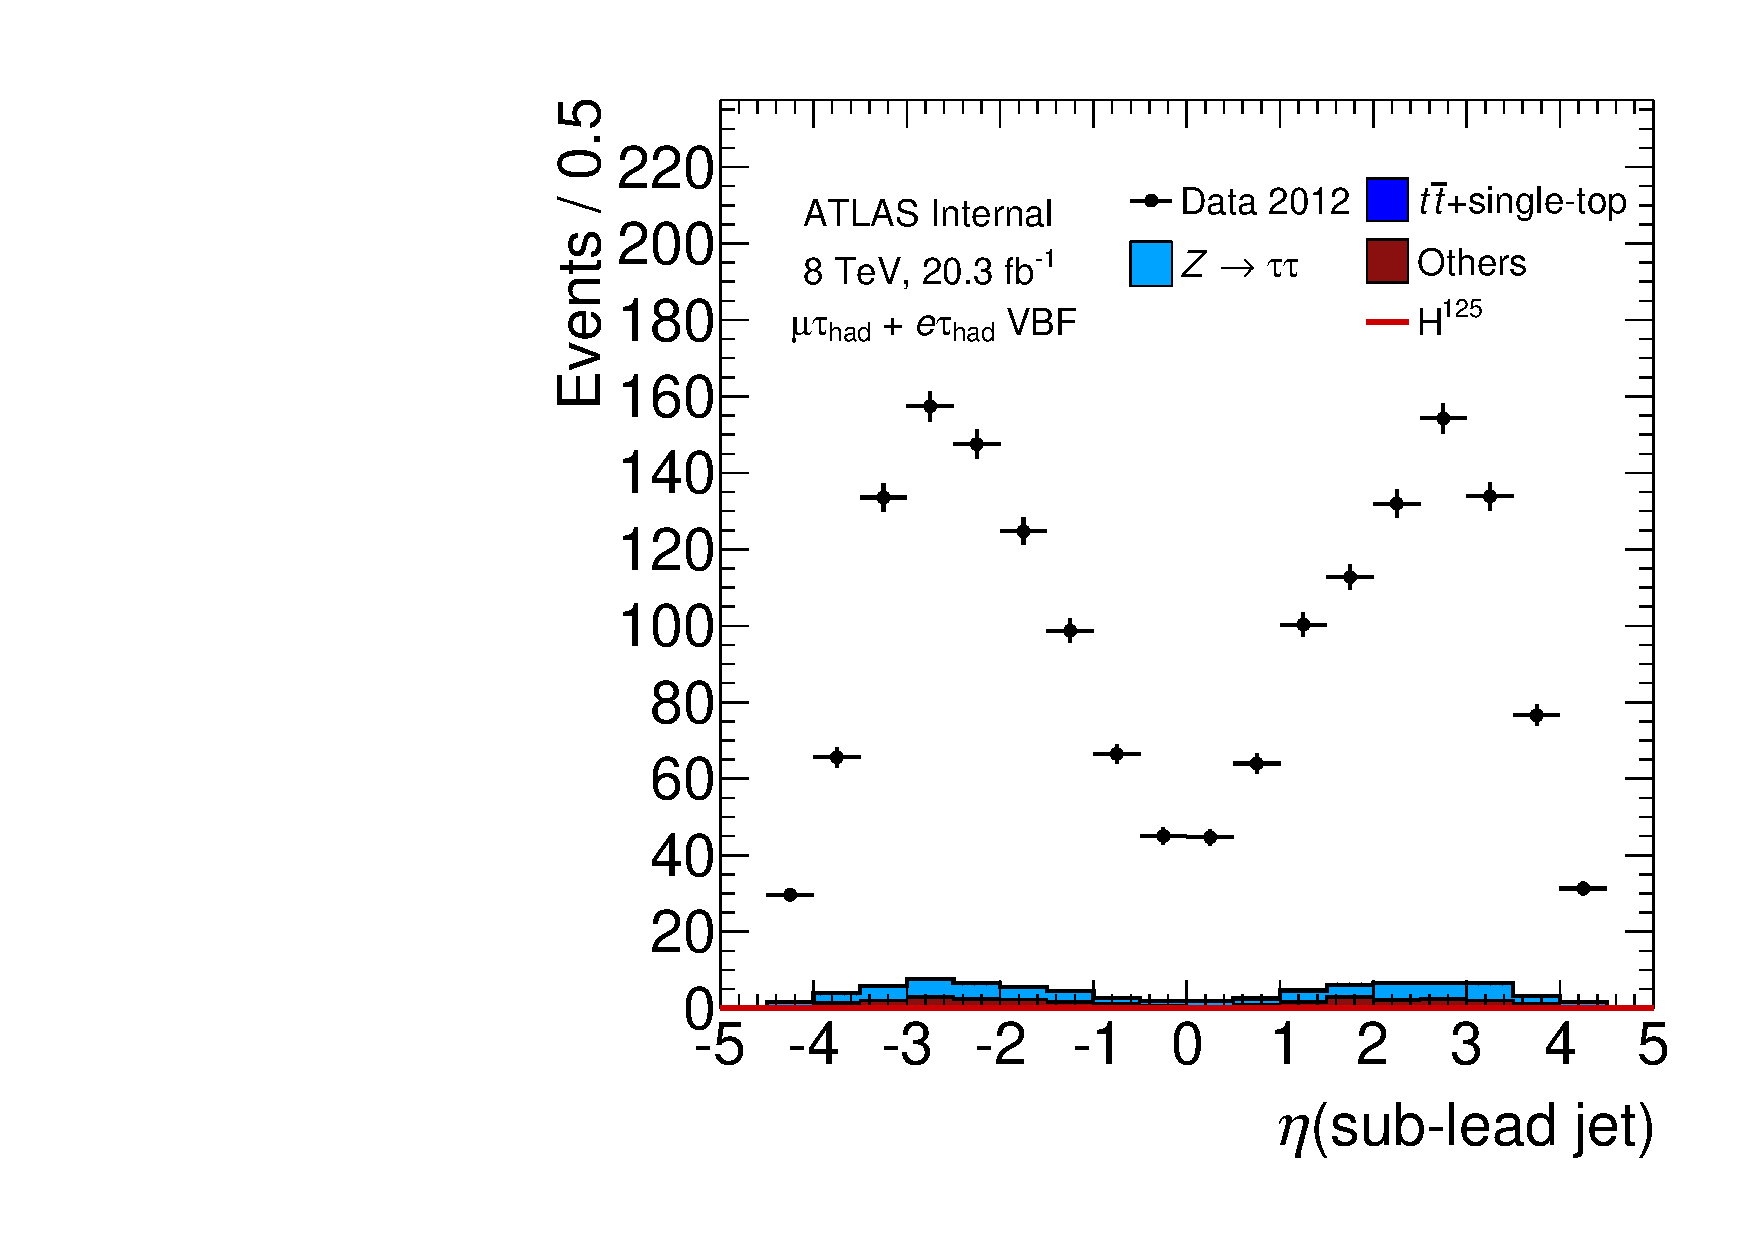
\includegraphics[width=0.32\textwidth]{figures/antitaus/jet-2-eta}
  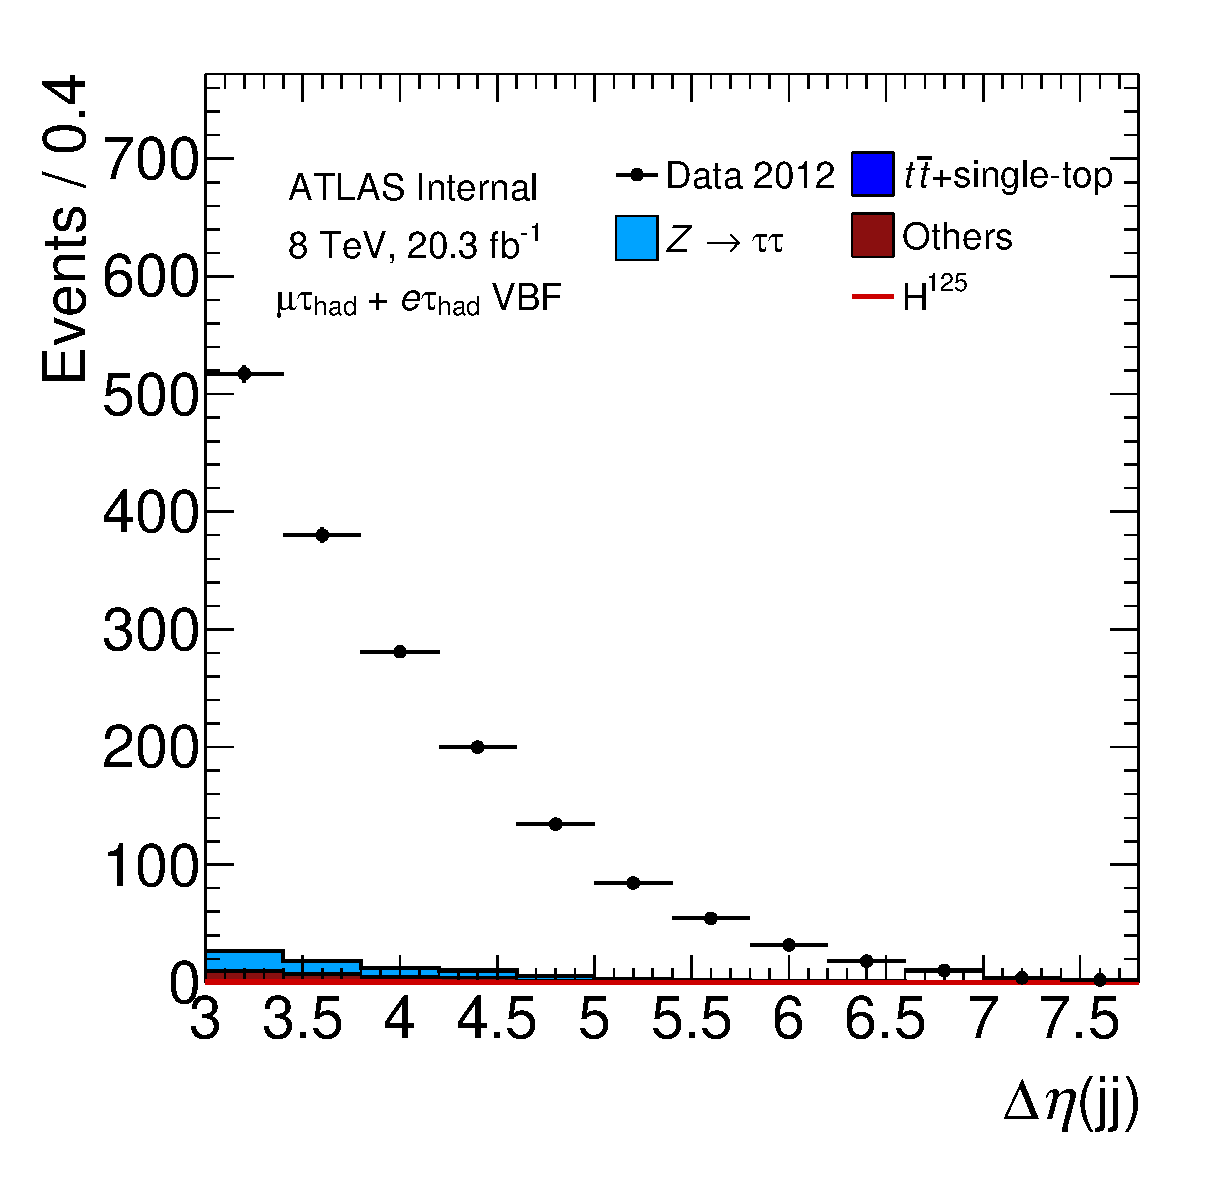
\includegraphics[width=0.32\textwidth]{figures/antitaus/jets-deta}
  % --------------
  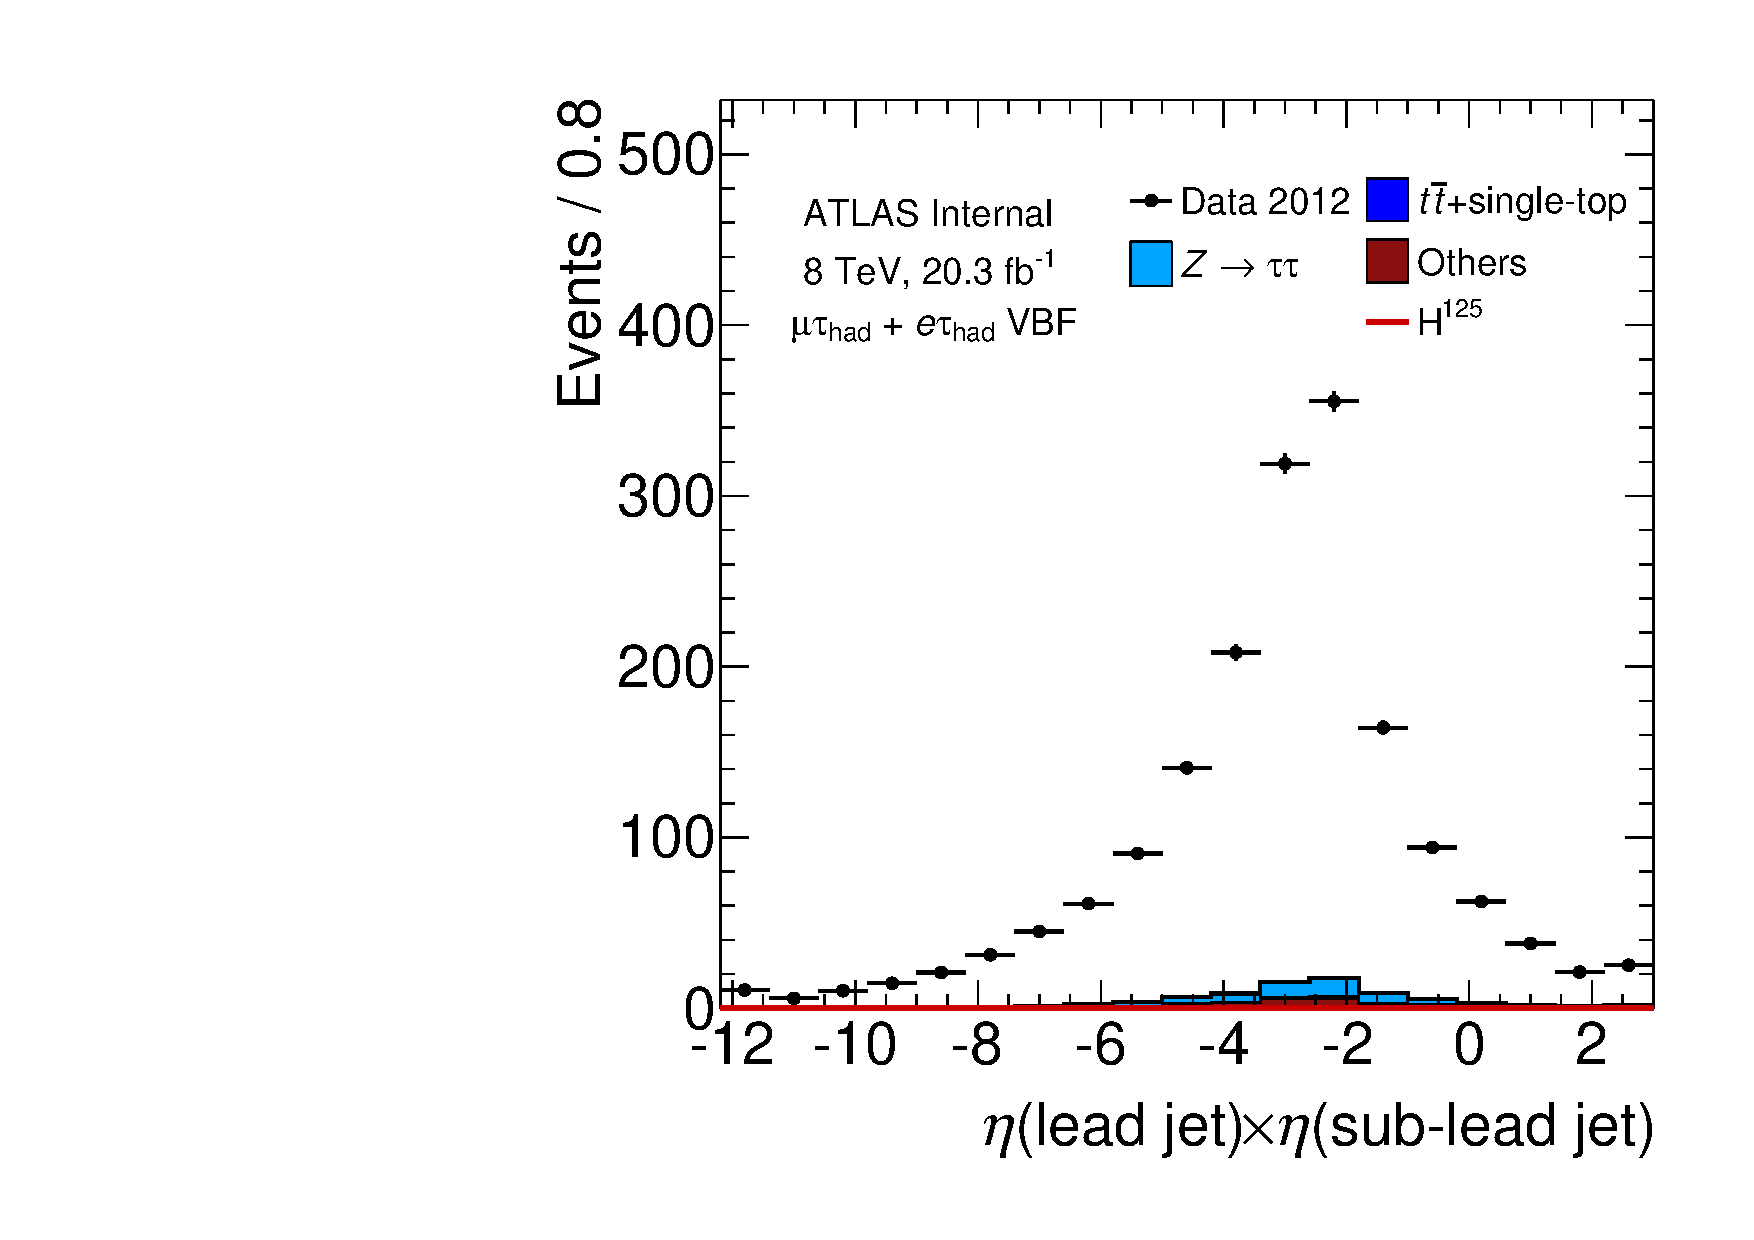
\includegraphics[width=0.32\textwidth]{figures/antitaus/jets-etaprod}
  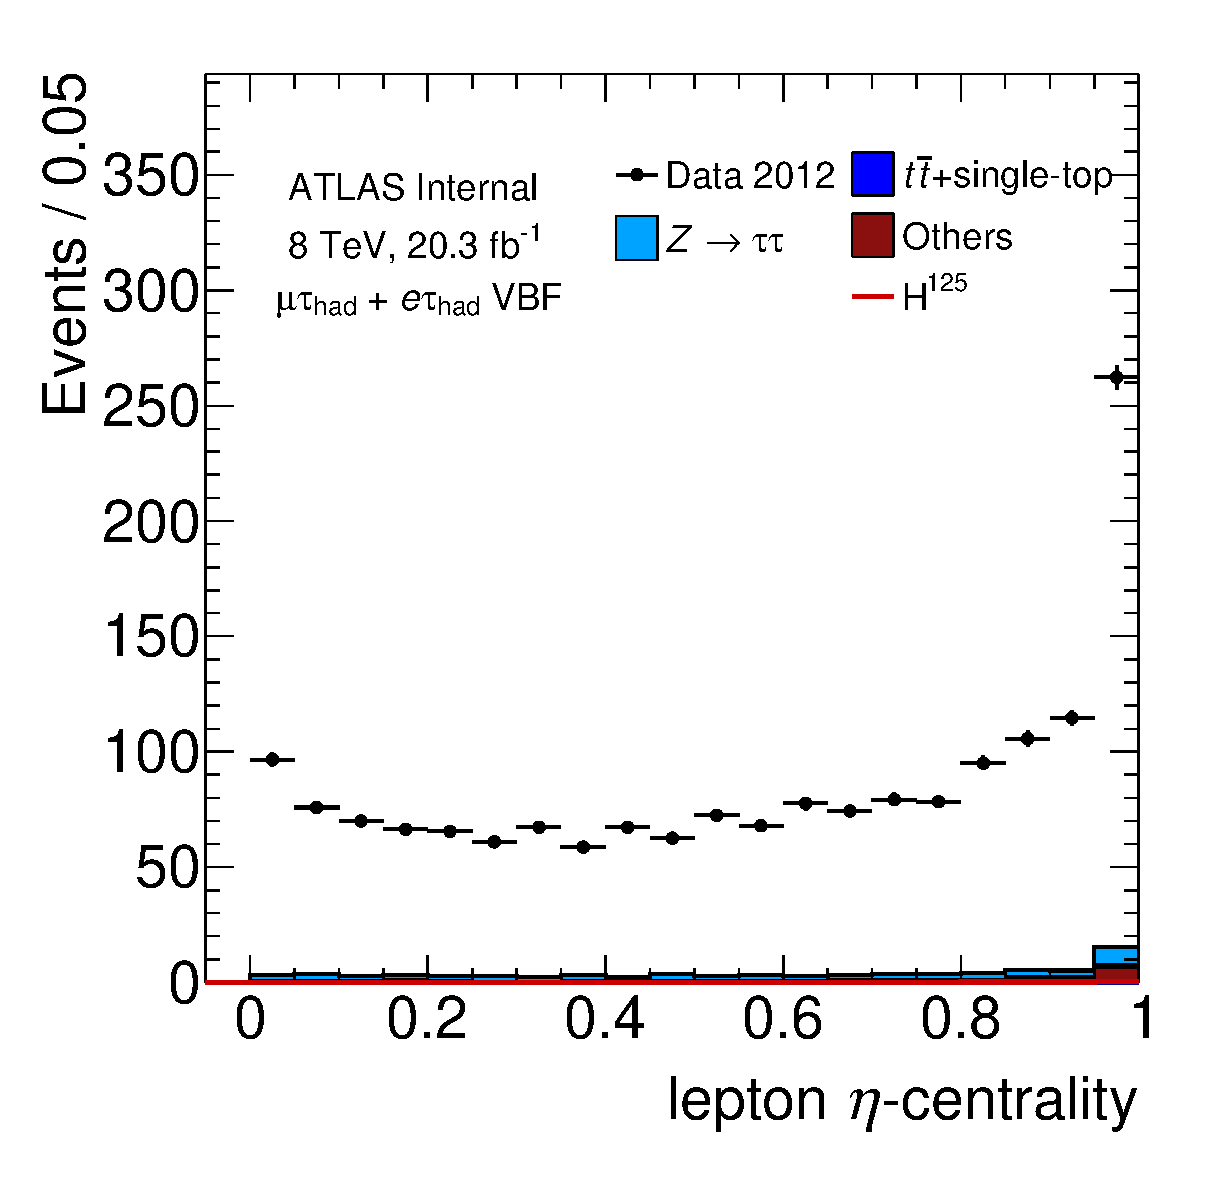
\includegraphics[width=0.32\textwidth]{figures/antitaus/lep-eta-centrality}
  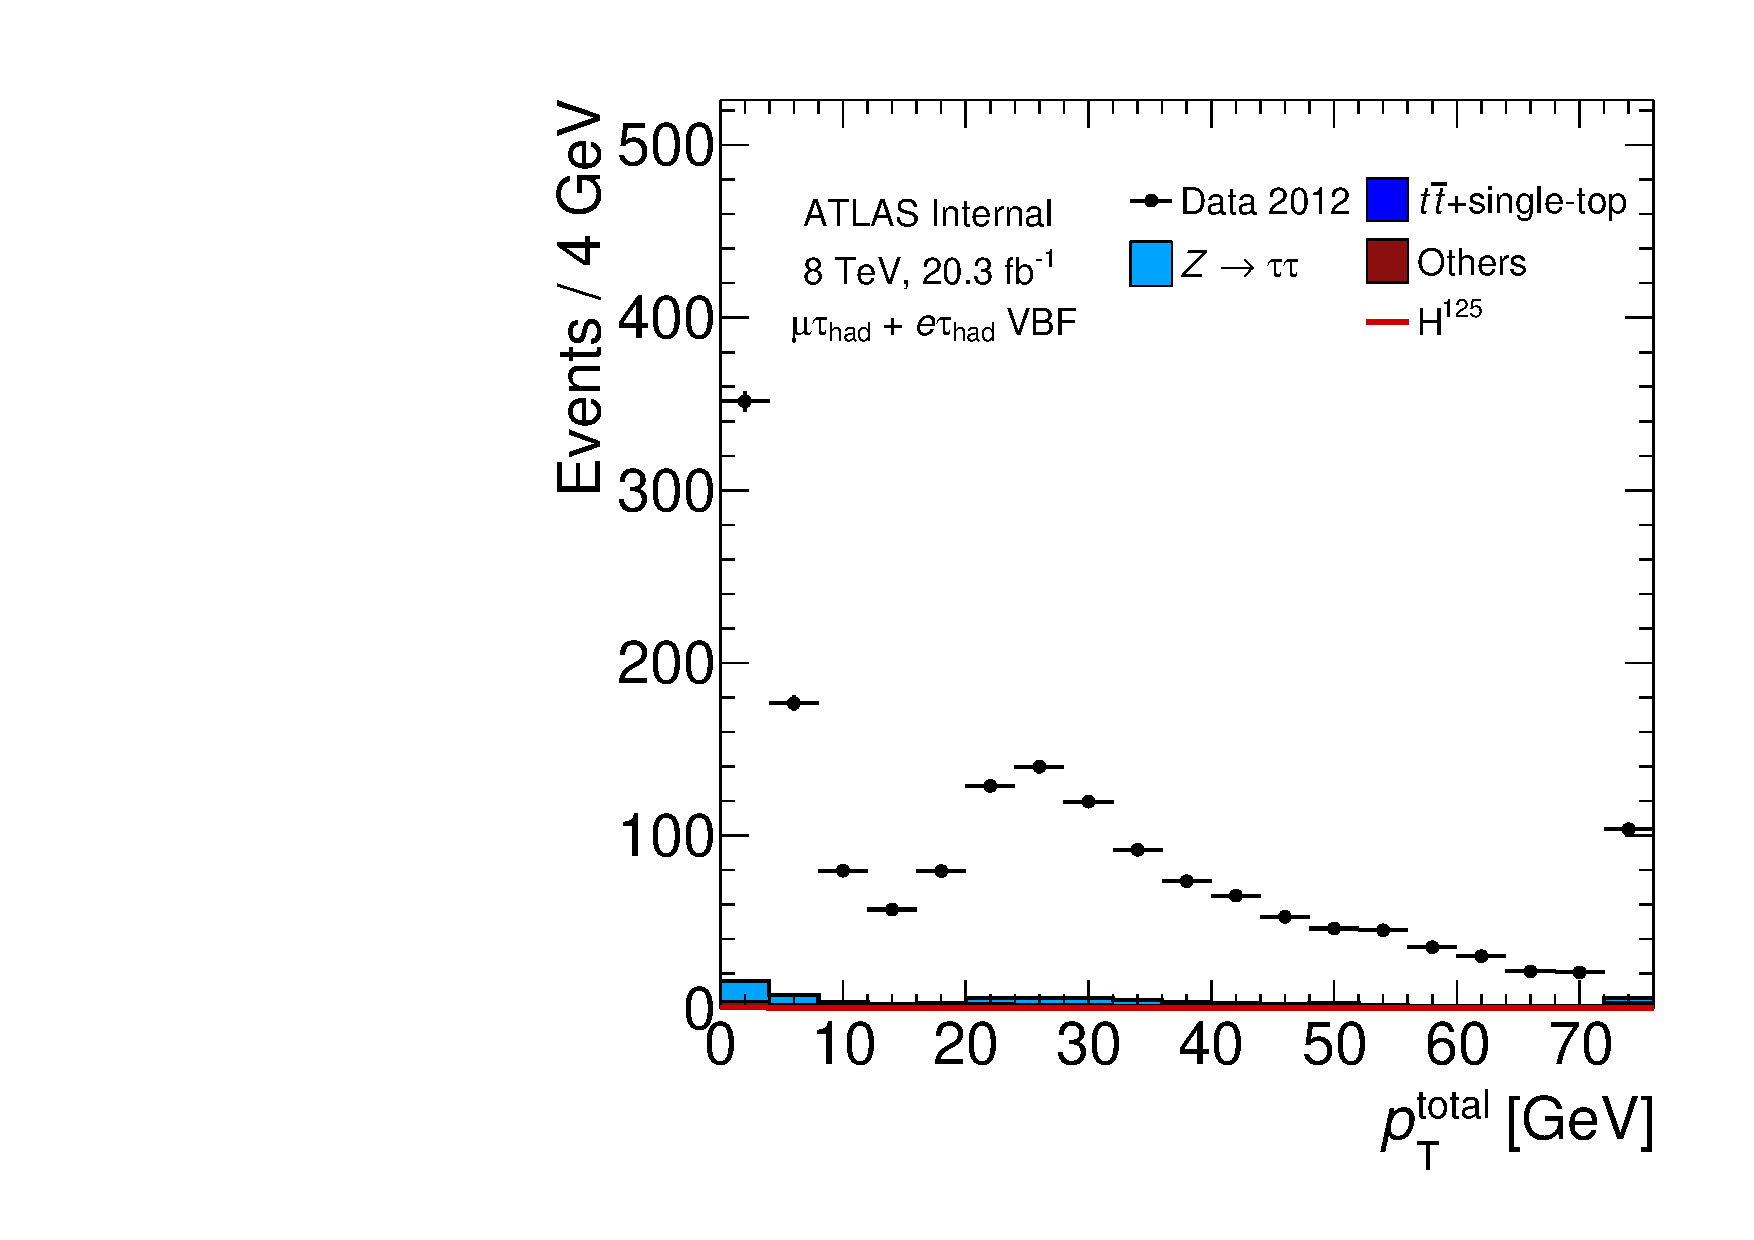
\includegraphics[width=0.32\textwidth]{figures/antitaus/system-pt}
  % --------------
  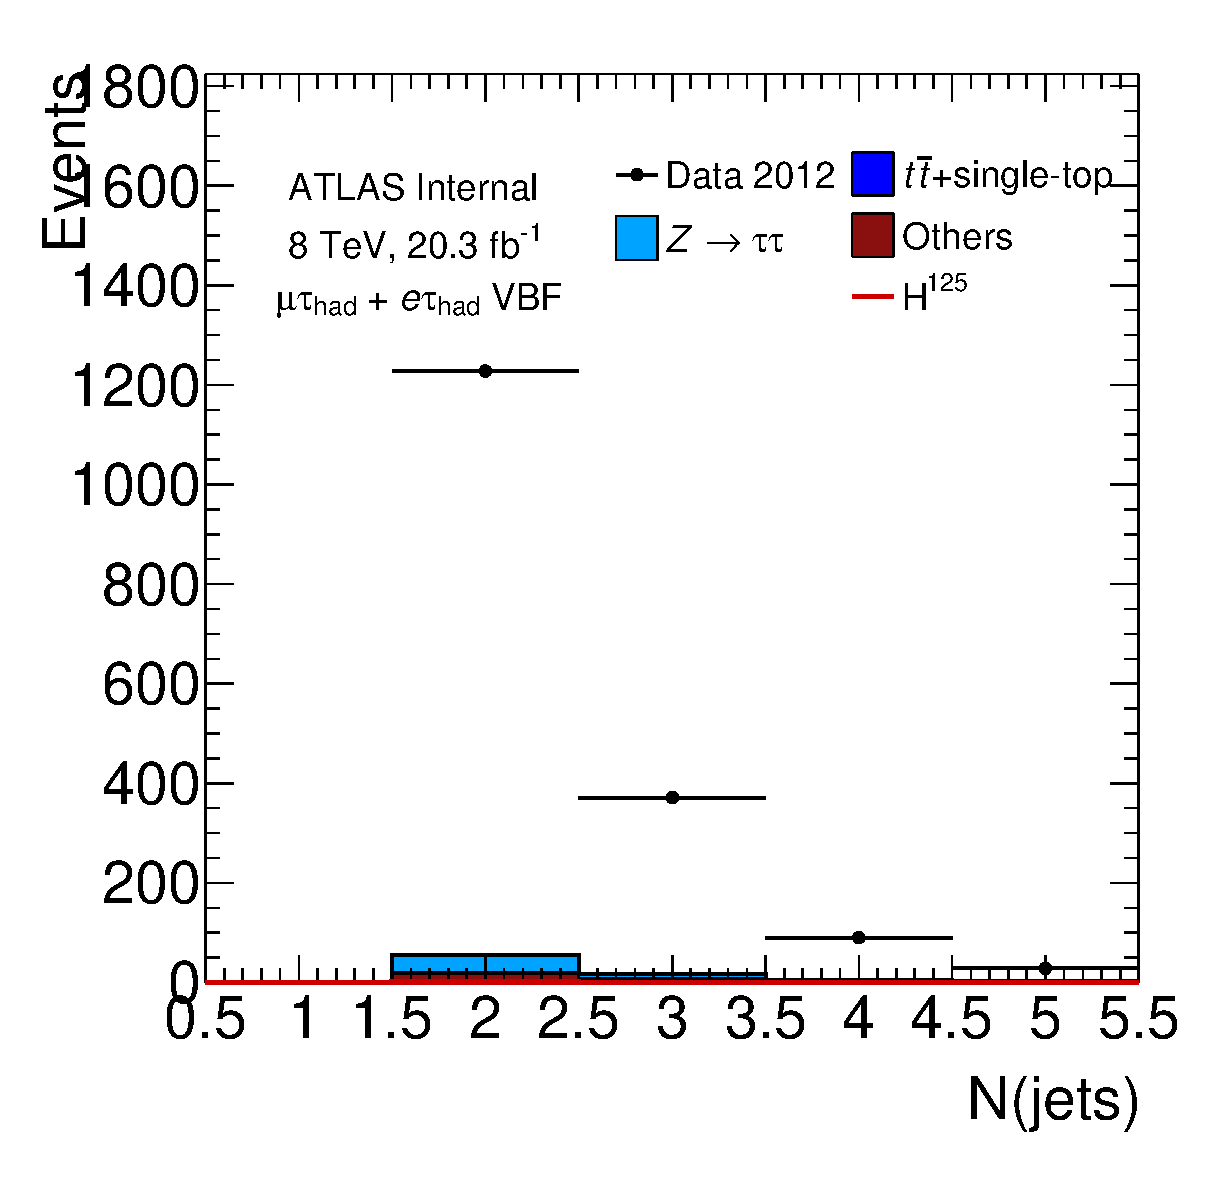
\includegraphics[width=0.32\textwidth]{figures/antitaus/n-jets30}
  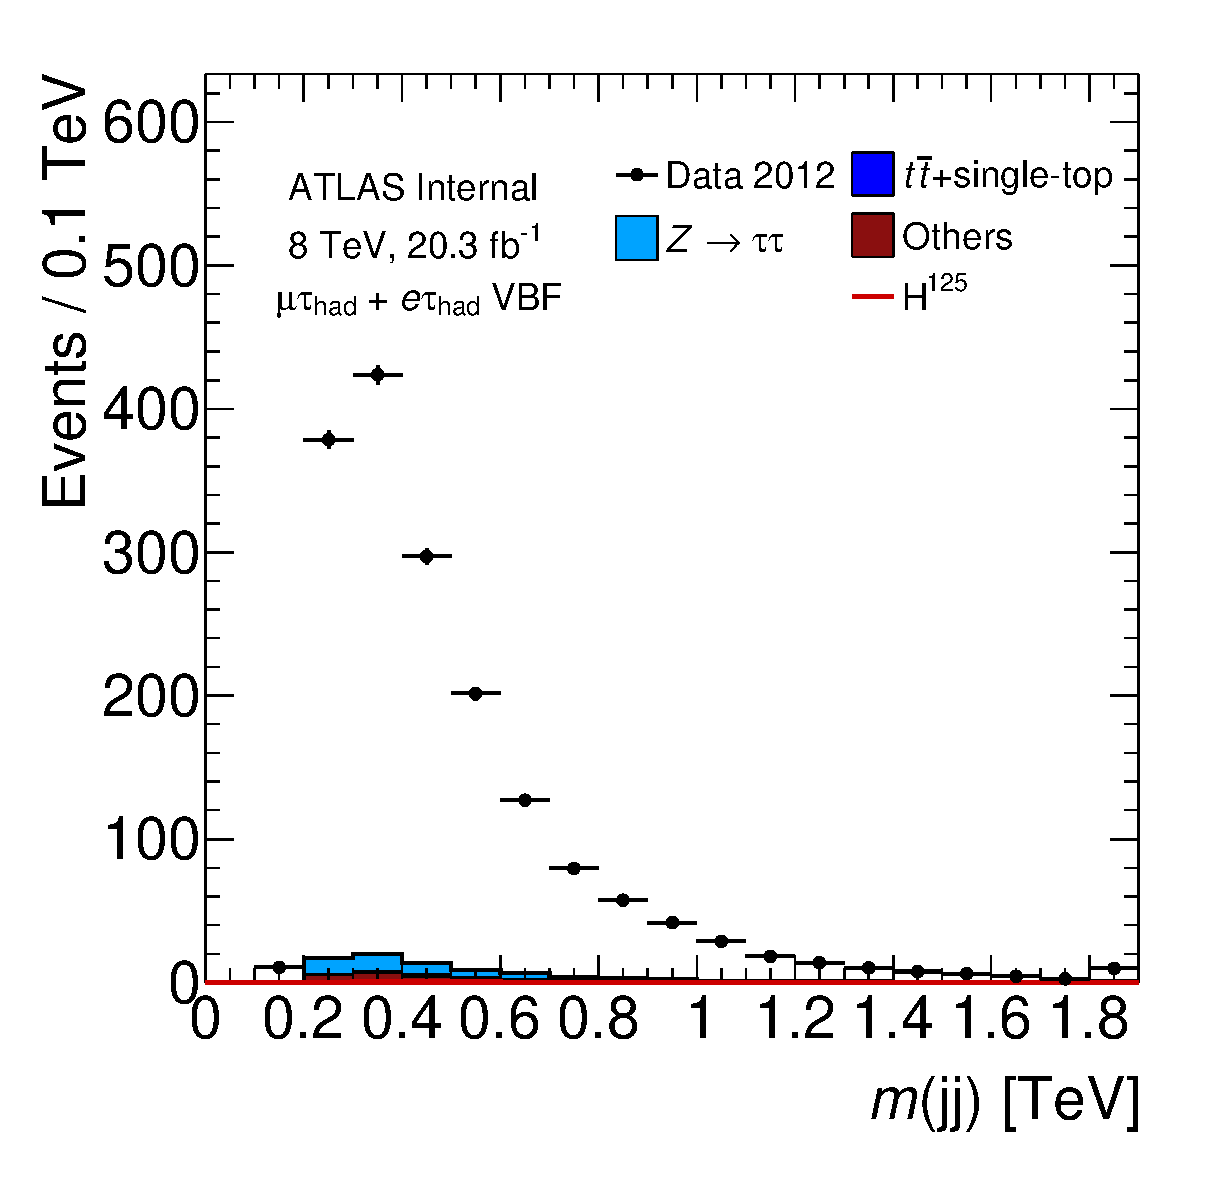
\includegraphics[width=0.32\textwidth]{figures/antitaus/dijet-m-veryhigh}
  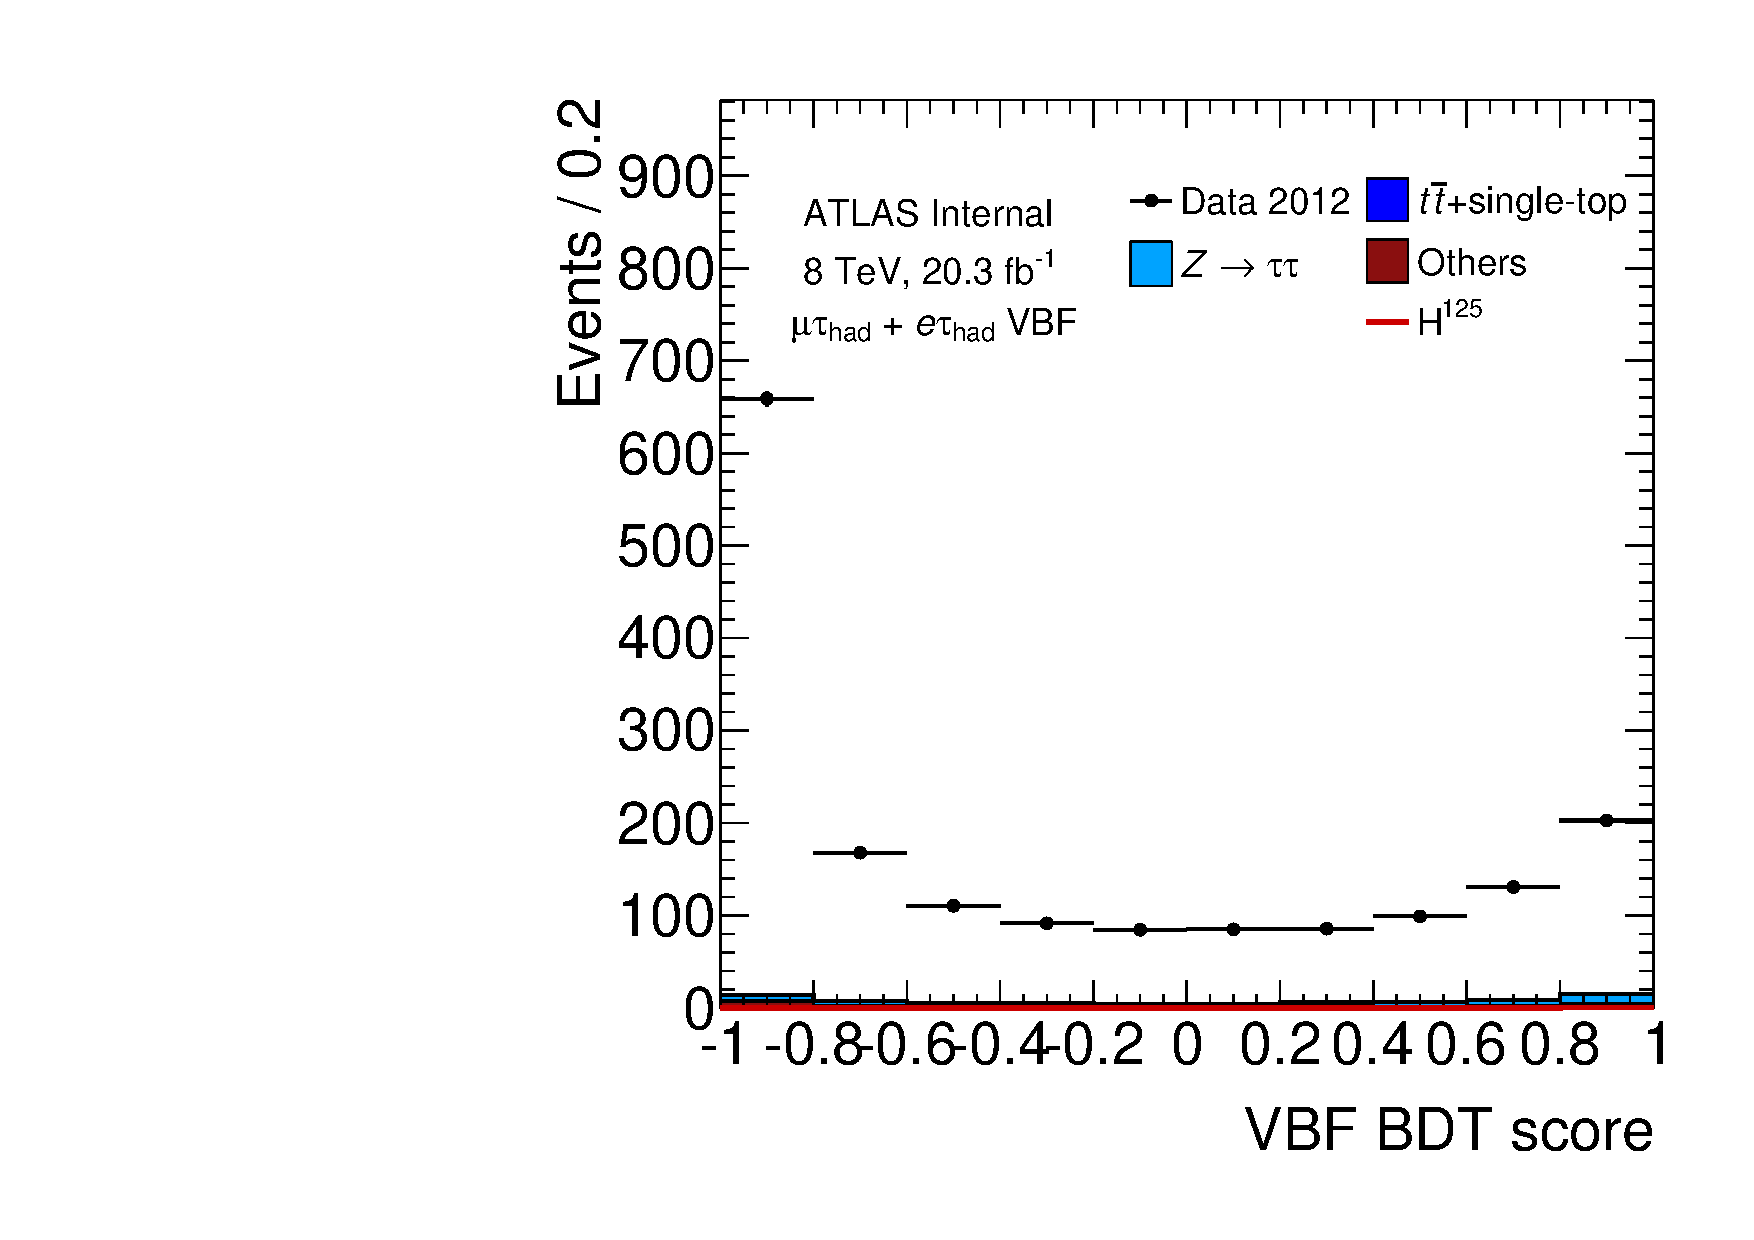
\includegraphics[width=0.32\textwidth]{figures/antitaus/BDTEve-VBF}
  \caption{Data events in the VBF category which fail $\tauh$ identification but fulfill all other requirements. The contamination of $\Ztautaulh$ and other processes without $\fakes$ is less than 10\%.}
  \label{fig:backgrounds-antitaus-jets}
\end{figure}

\clearpage

\begin{figure}[tp]
  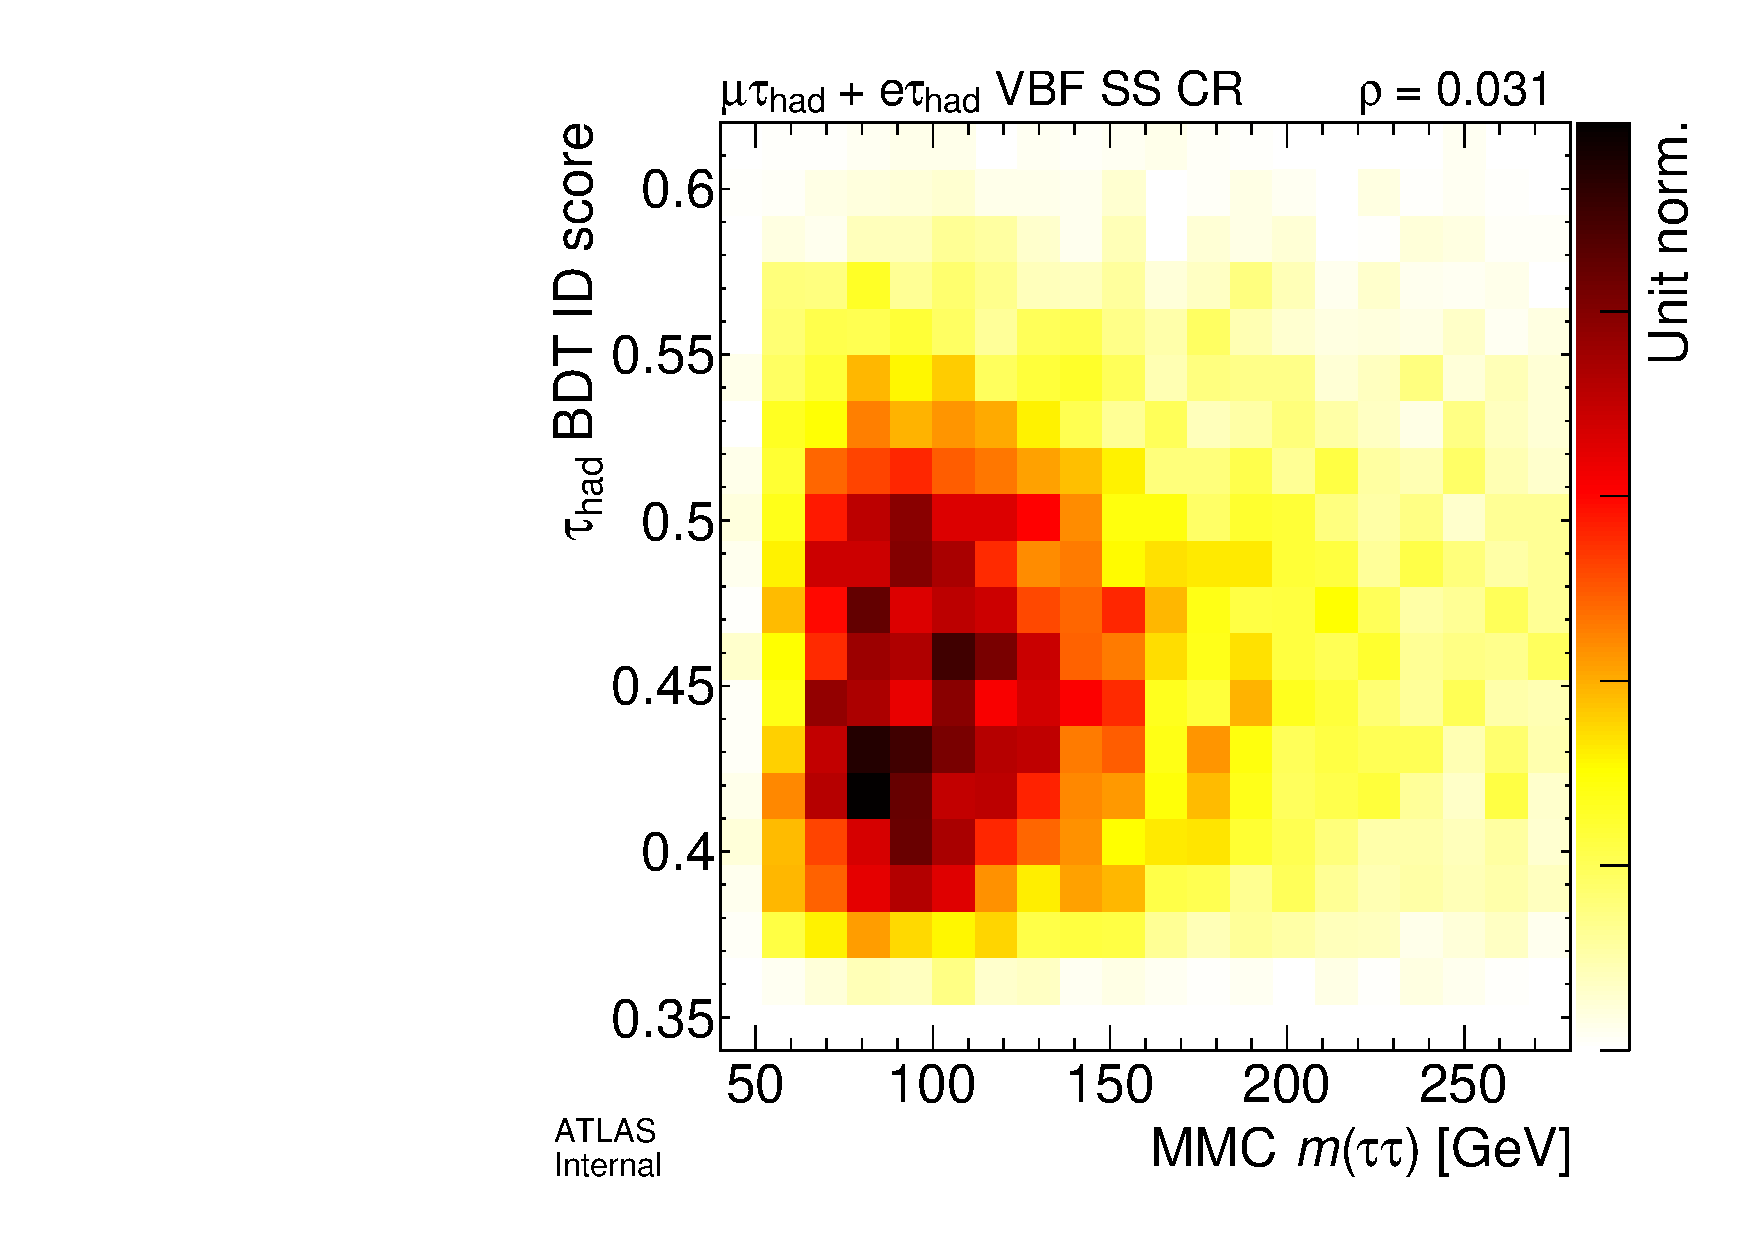
\includegraphics[width=0.32\textwidth]{figures/tauidcorrelations/tauid_vs_mMMC}
  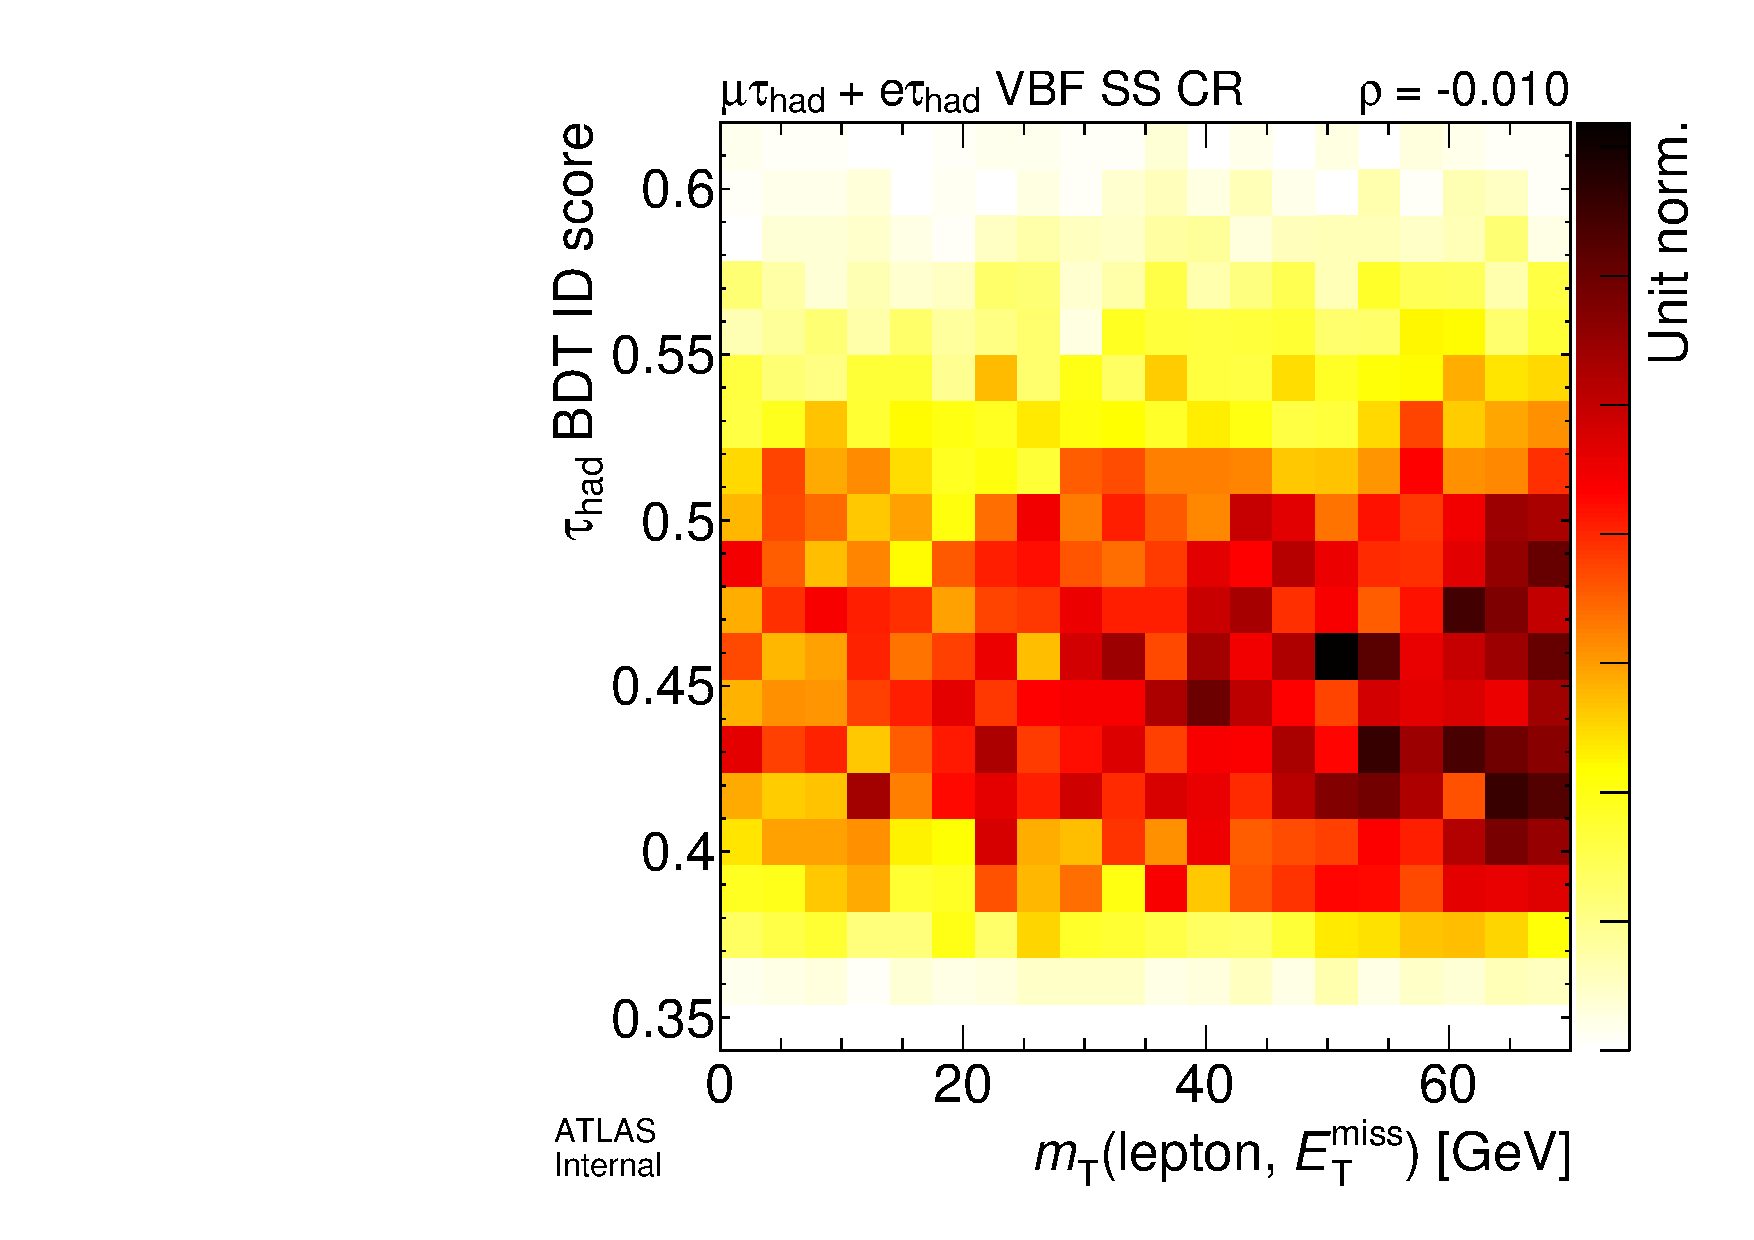
\includegraphics[width=0.32\textwidth]{figures/tauidcorrelations/tauid_vs_mT}
  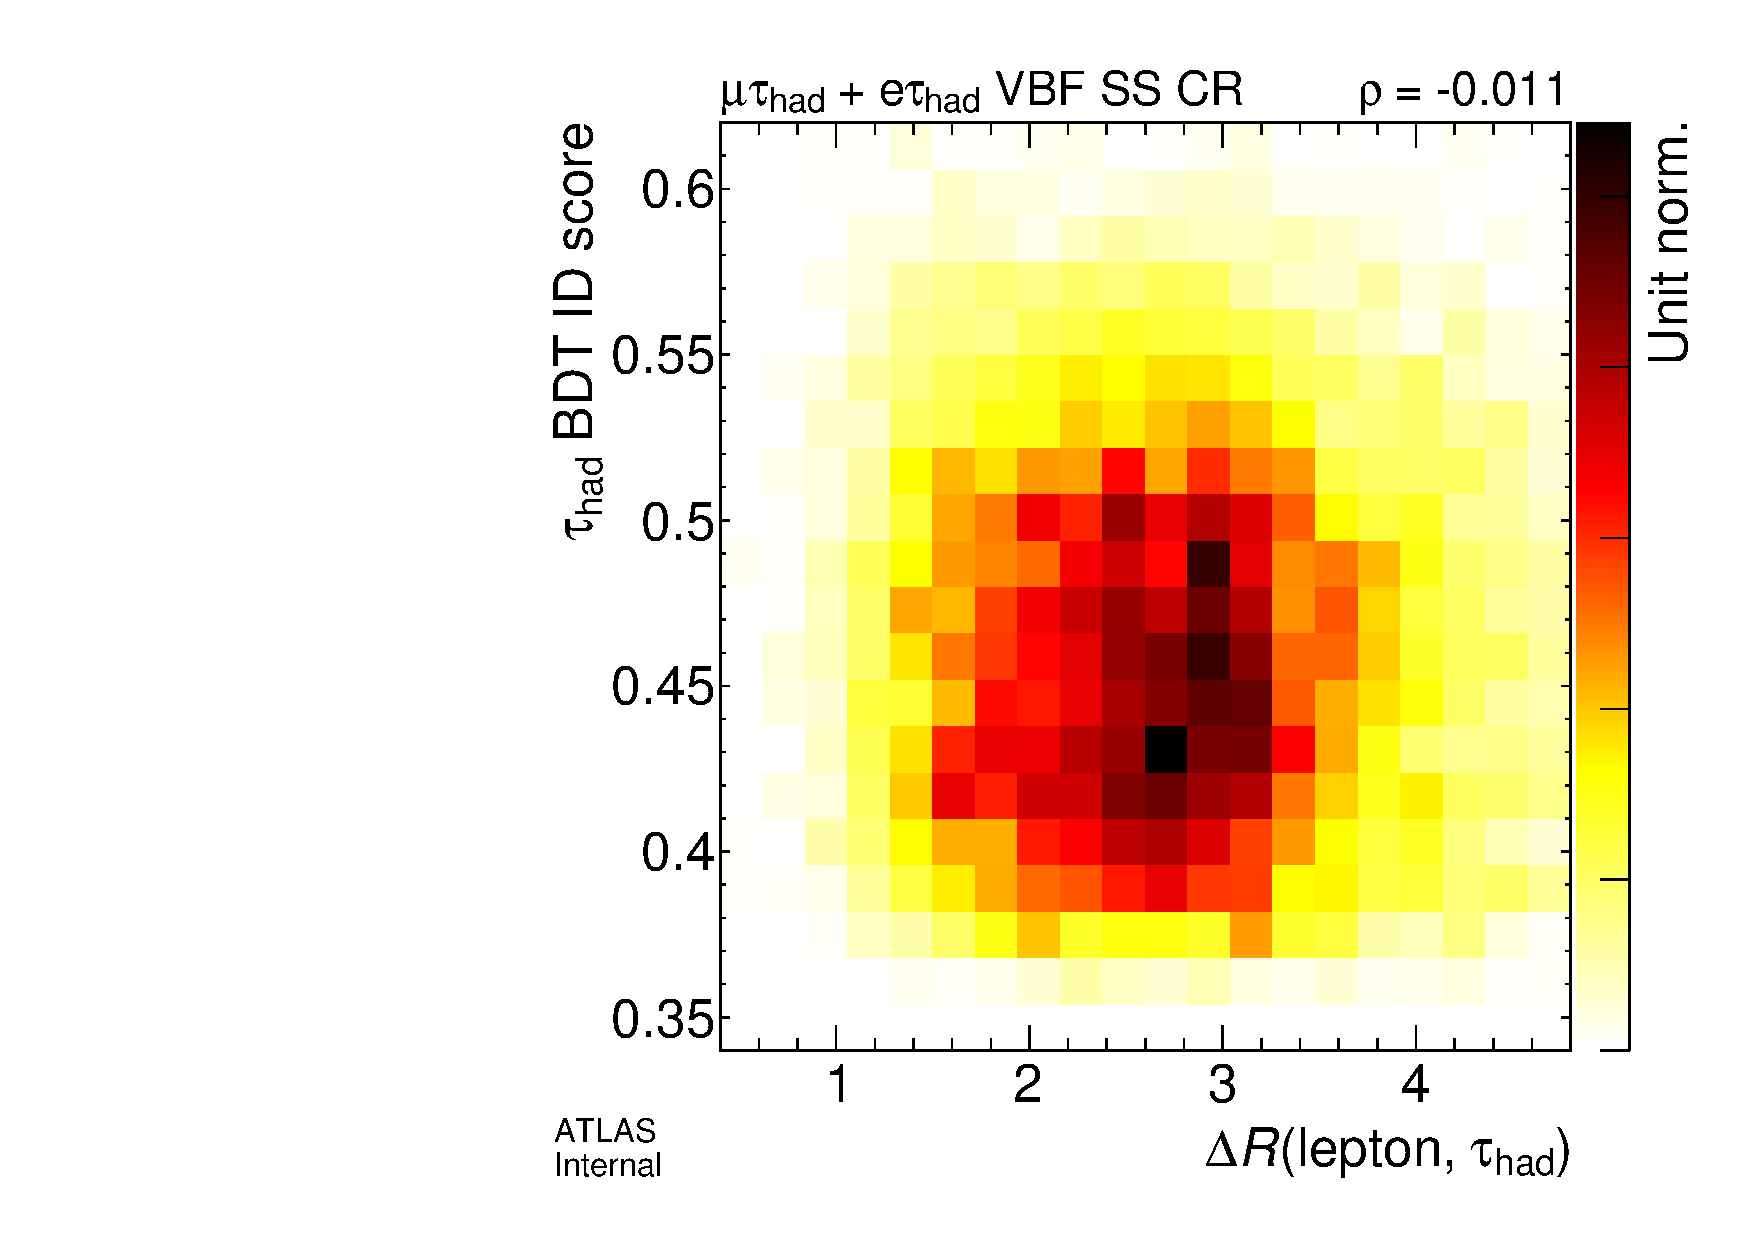
\includegraphics[width=0.32\textwidth]{figures/tauidcorrelations/tauid_vs_dR}
  % --------------
  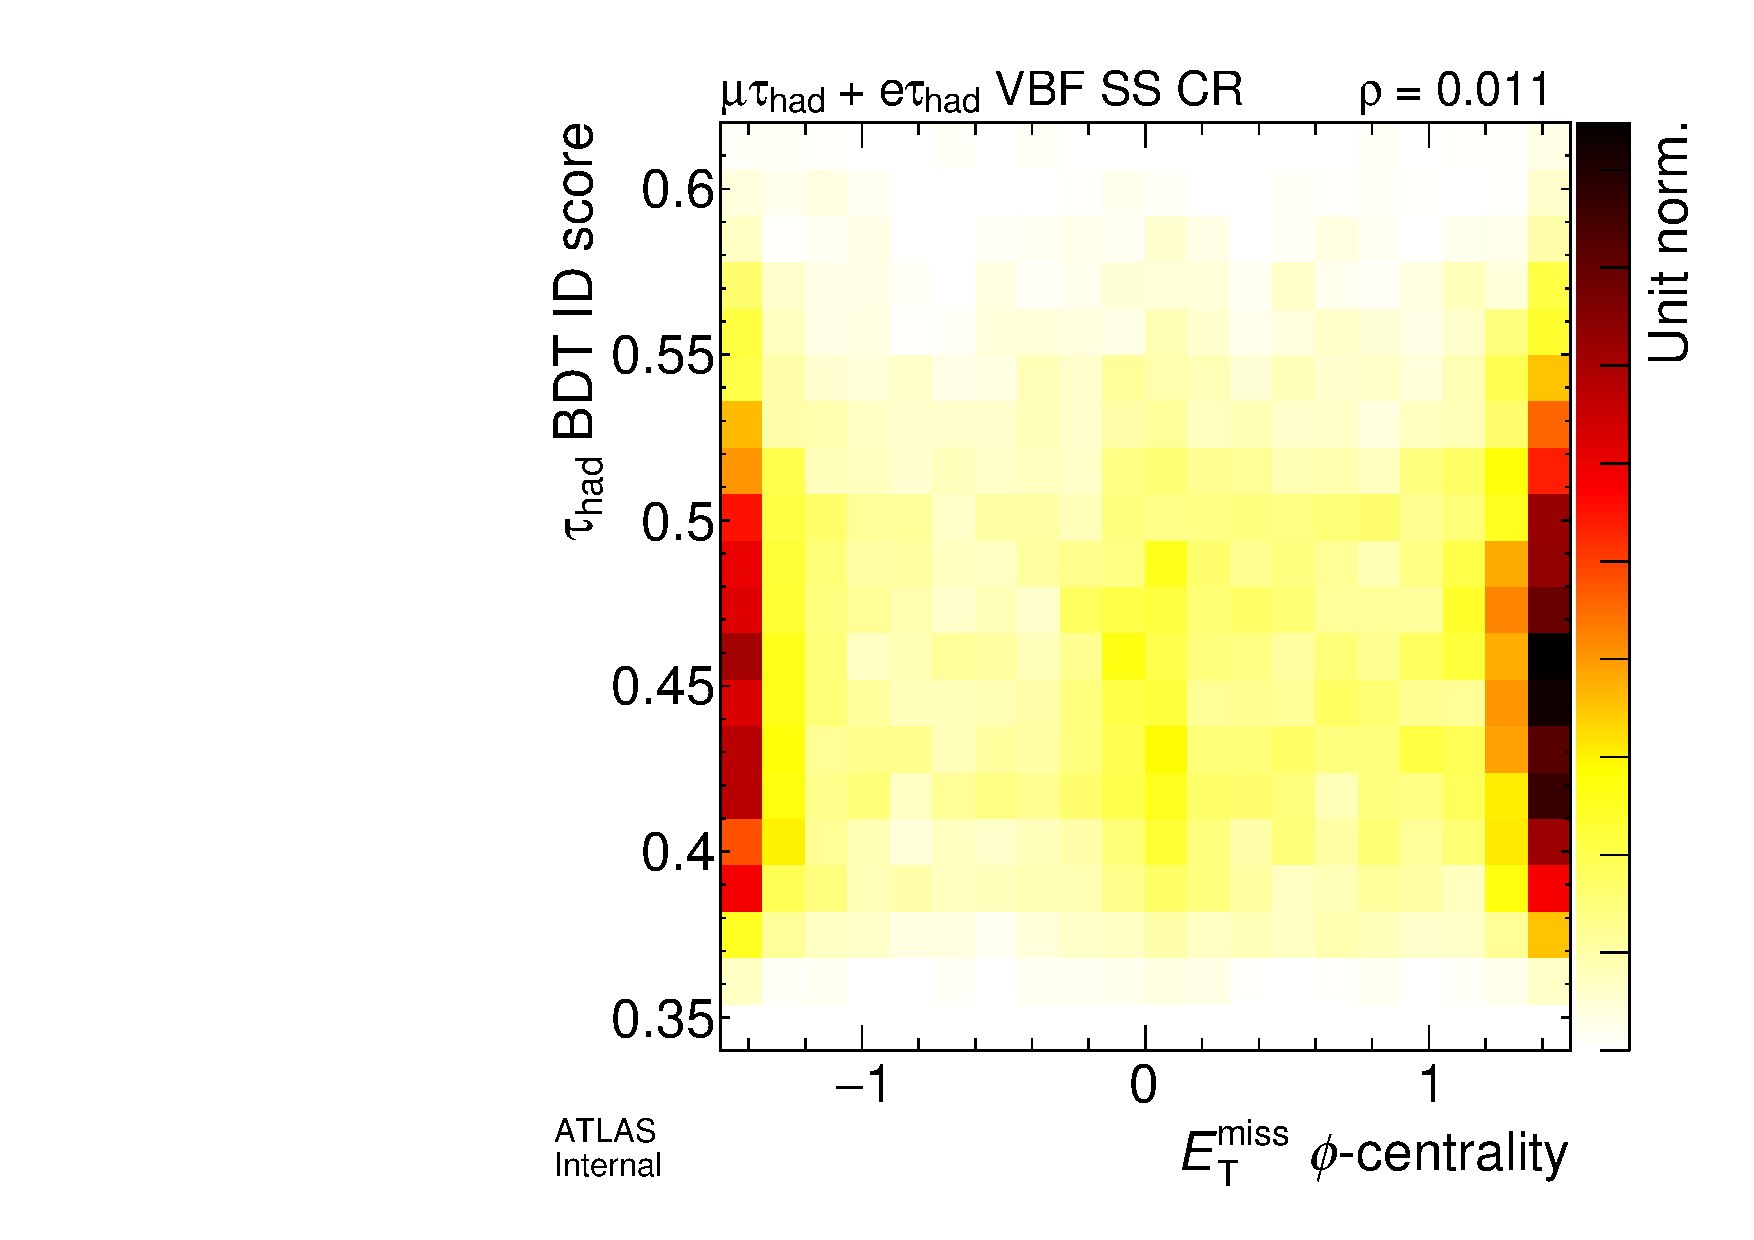
\includegraphics[width=0.32\textwidth]{figures/tauidcorrelations/tauid_vs_metphi}
  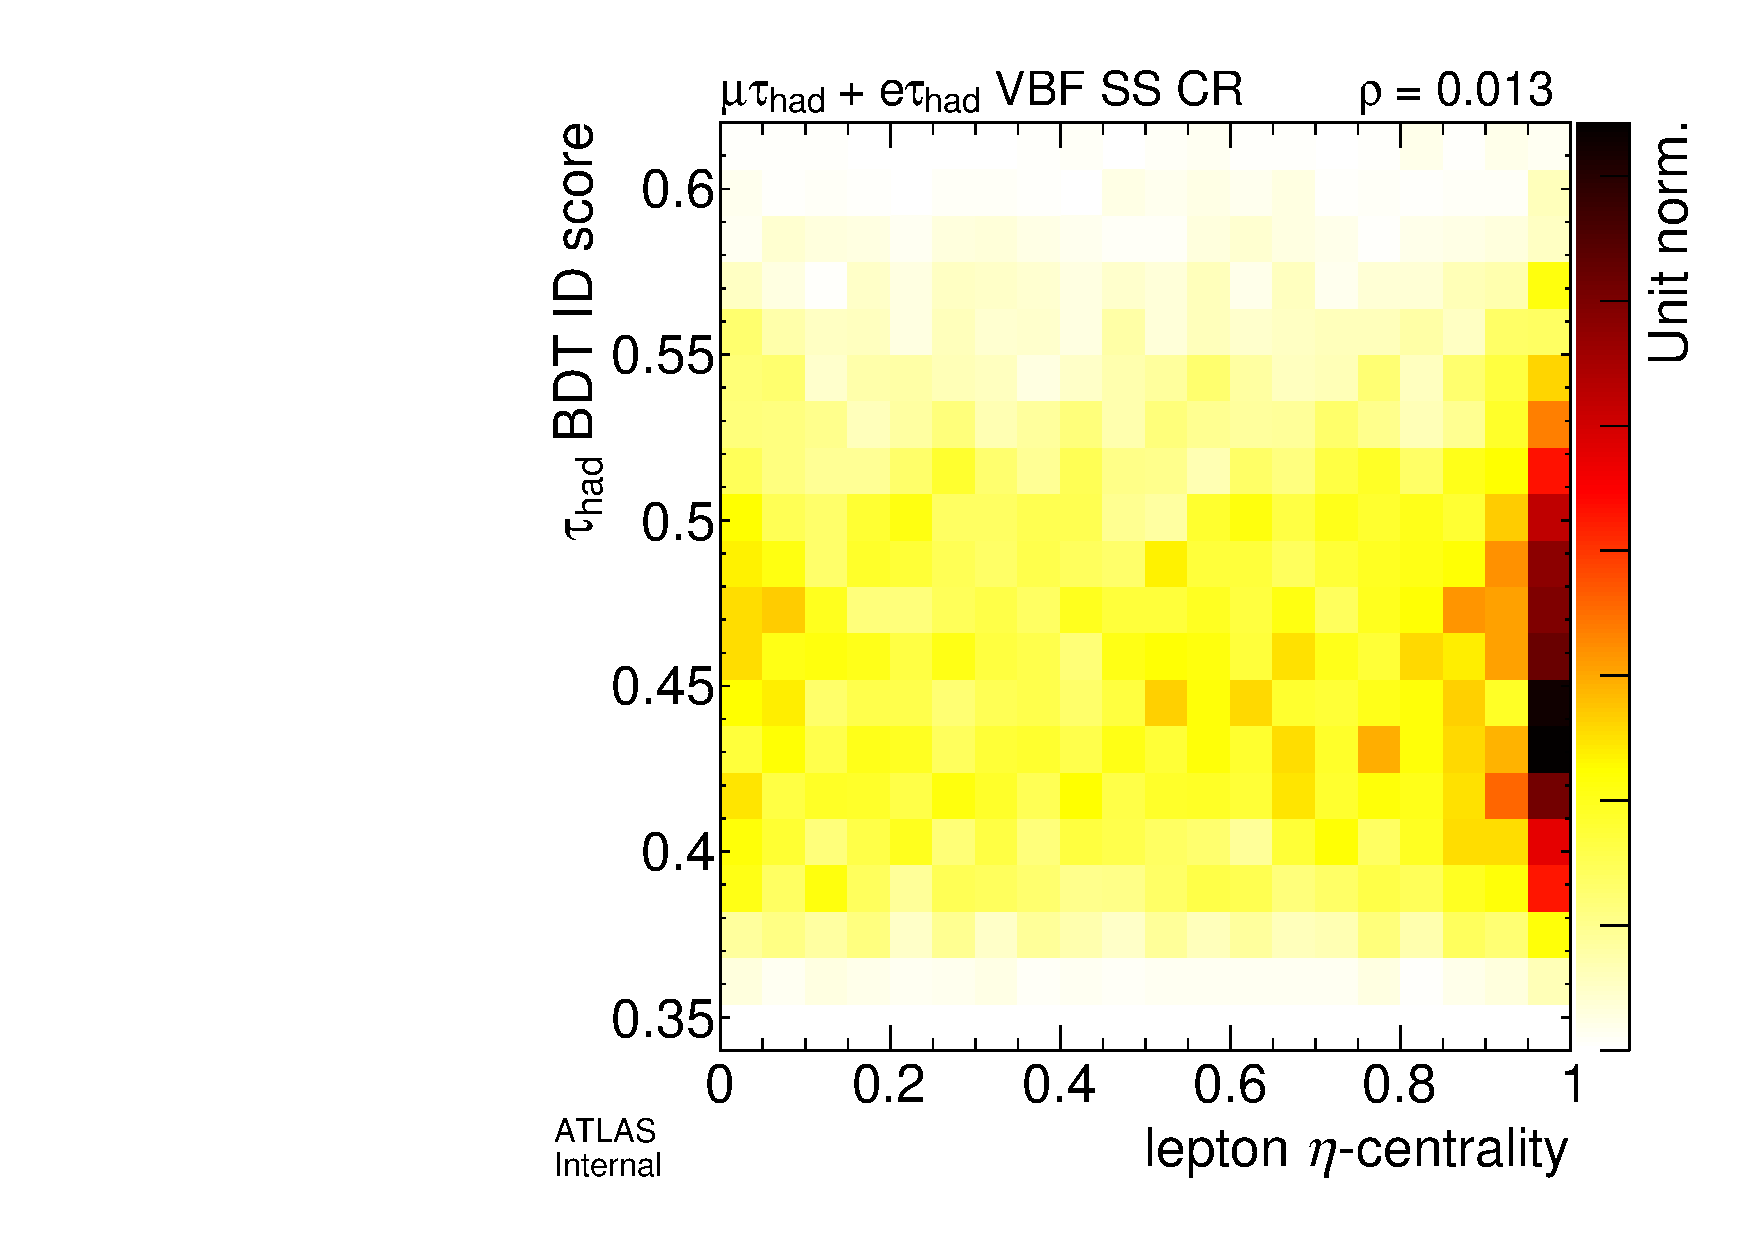
\includegraphics[width=0.32\textwidth]{figures/tauidcorrelations/tauid_vs_lepeta}
  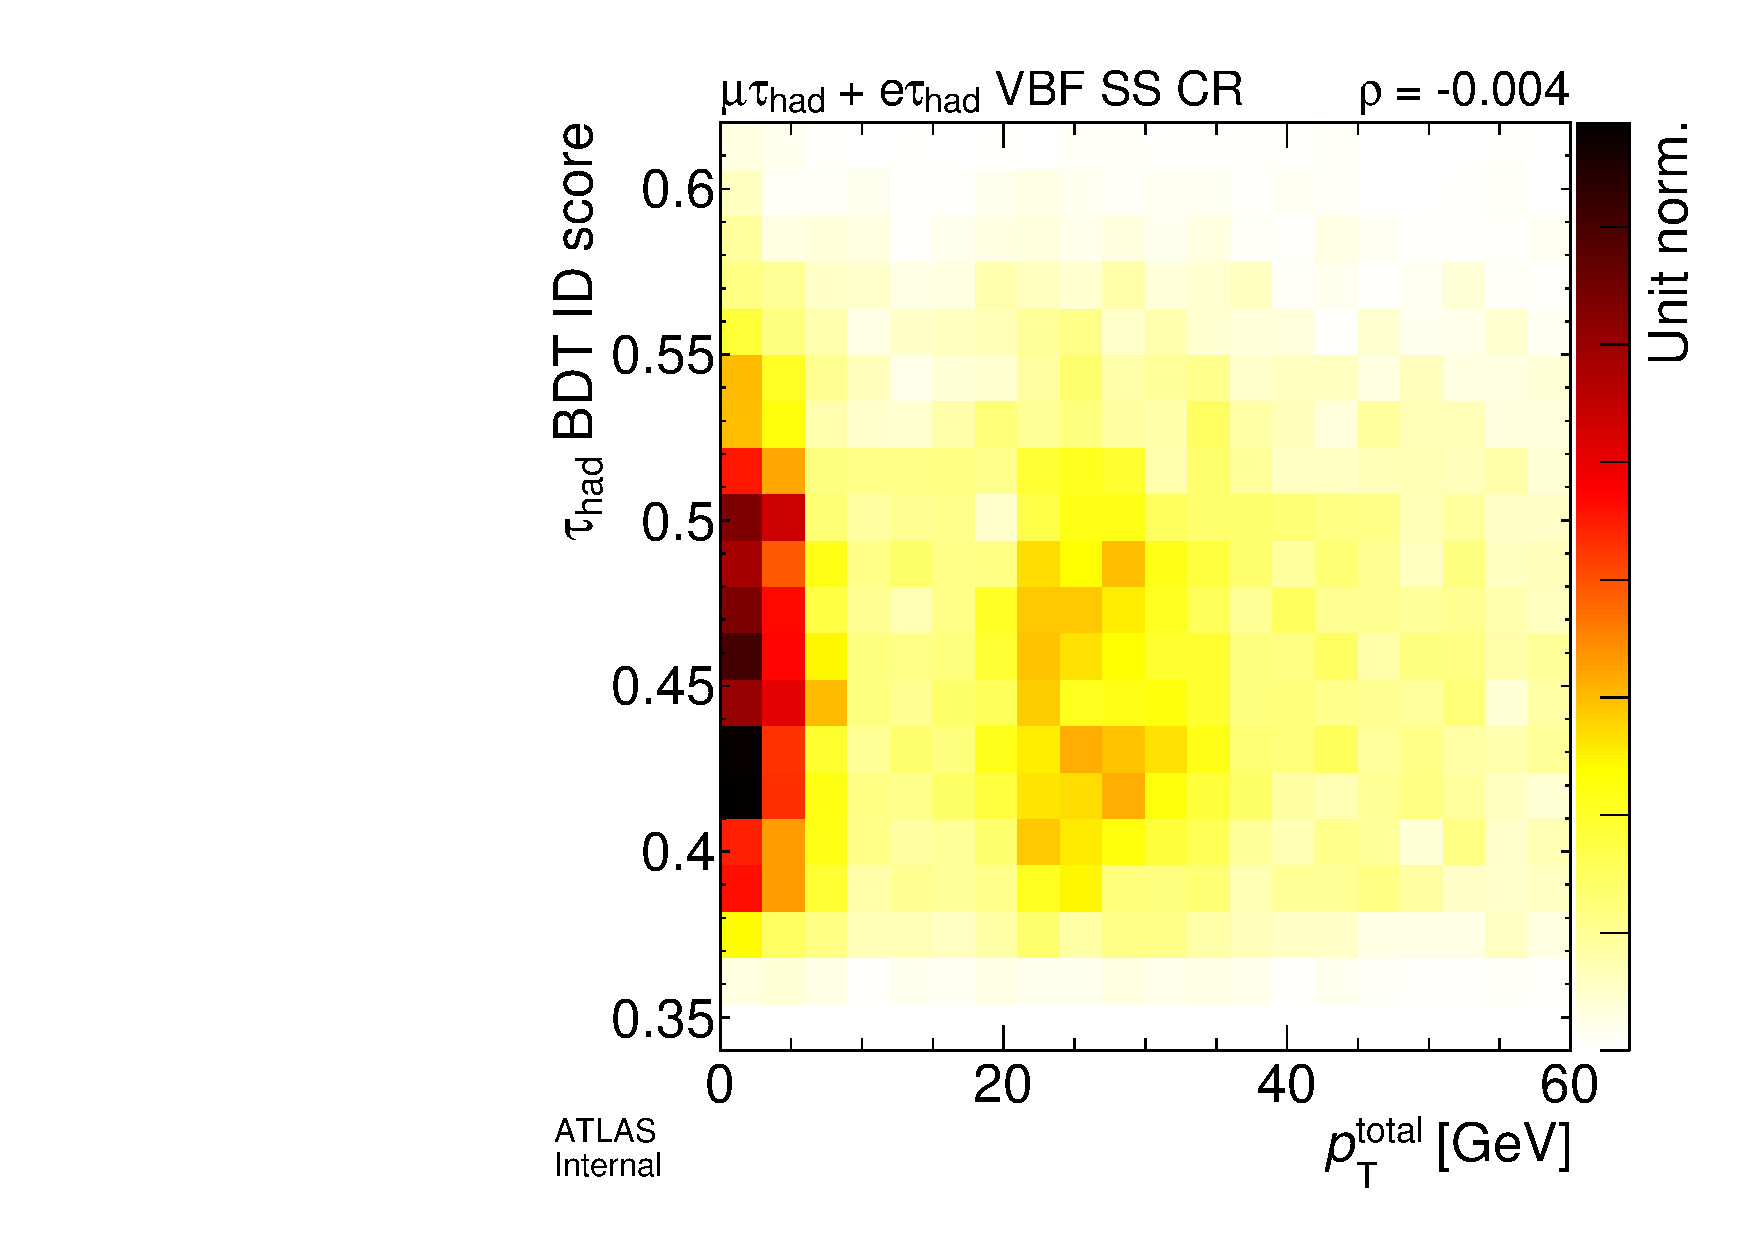
\includegraphics[width=0.32\textwidth]{figures/tauidcorrelations/tauid_vs_pttot}
  % --------------
  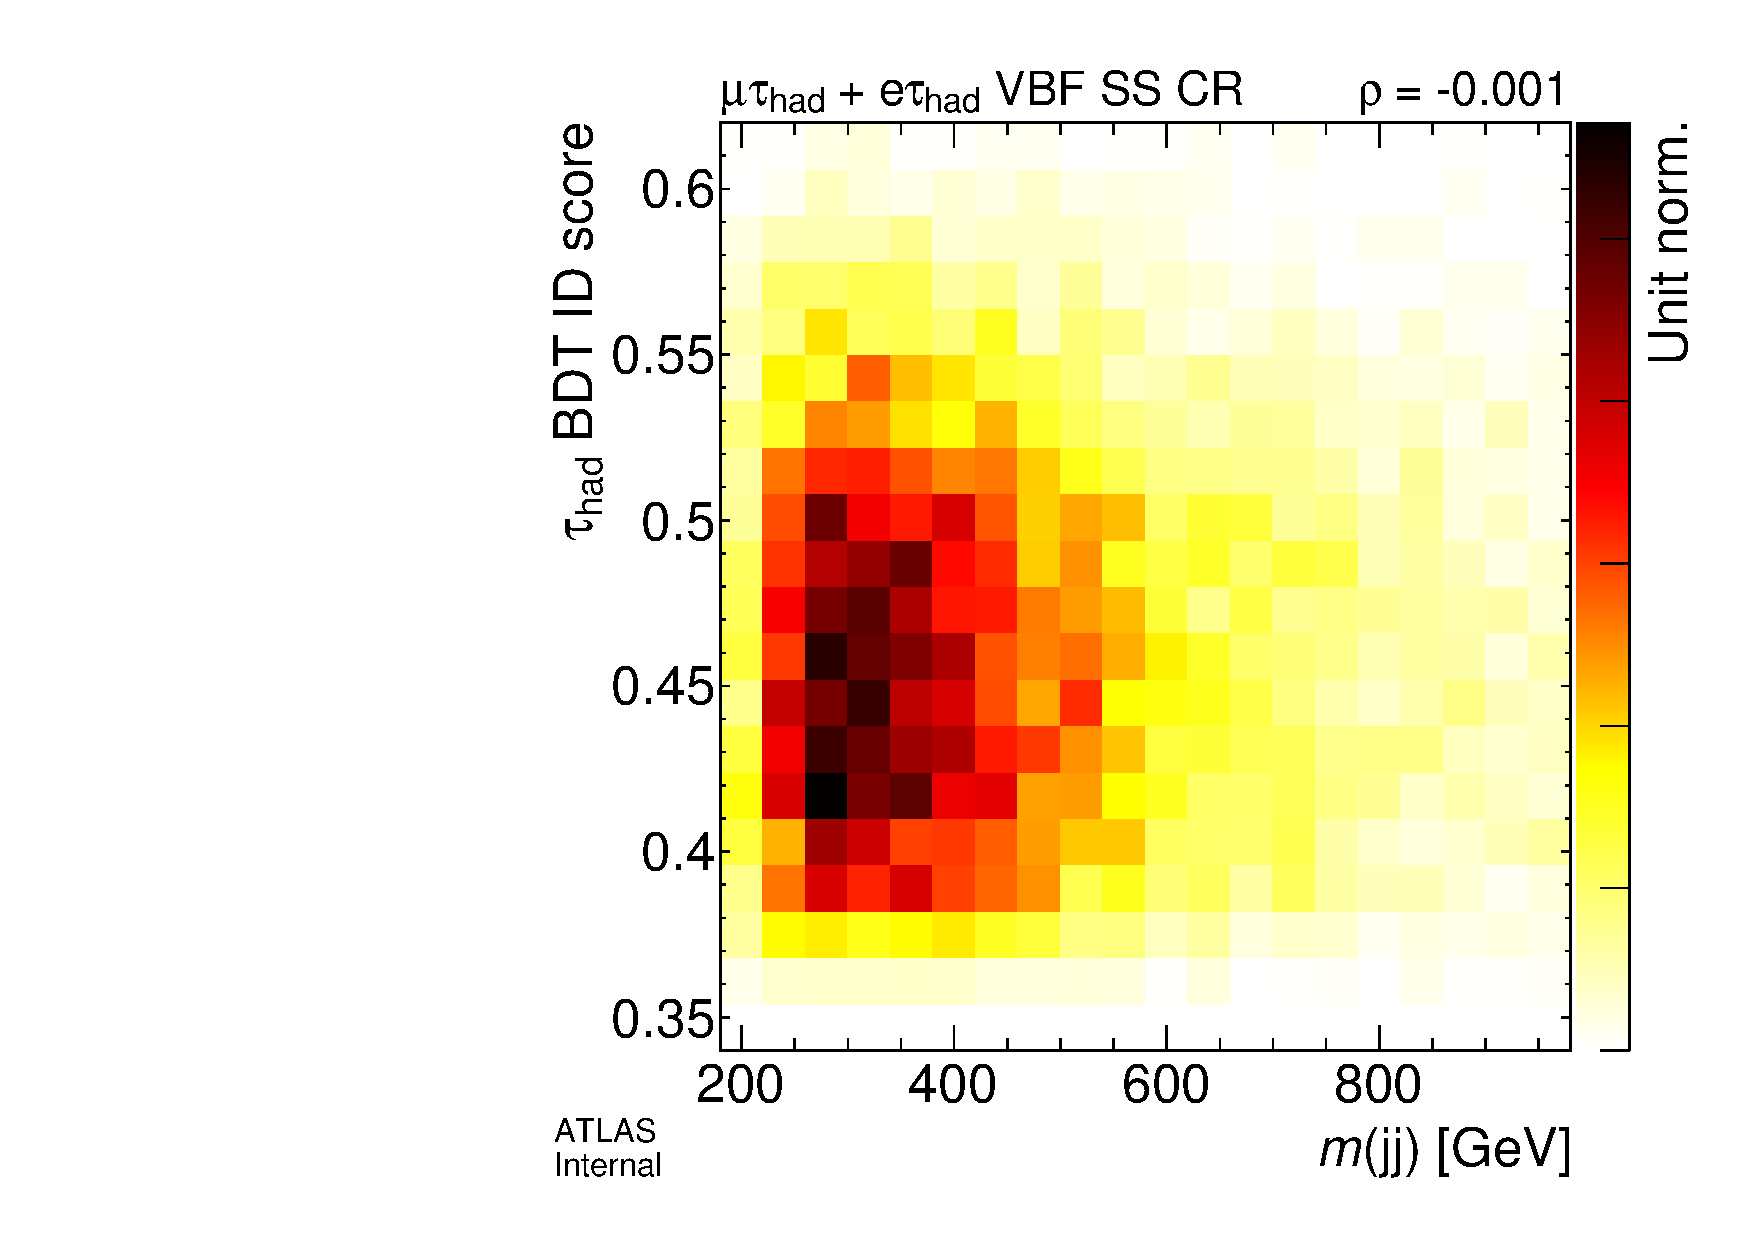
\includegraphics[width=0.32\textwidth]{figures/tauidcorrelations/tauid_vs_mjj}
  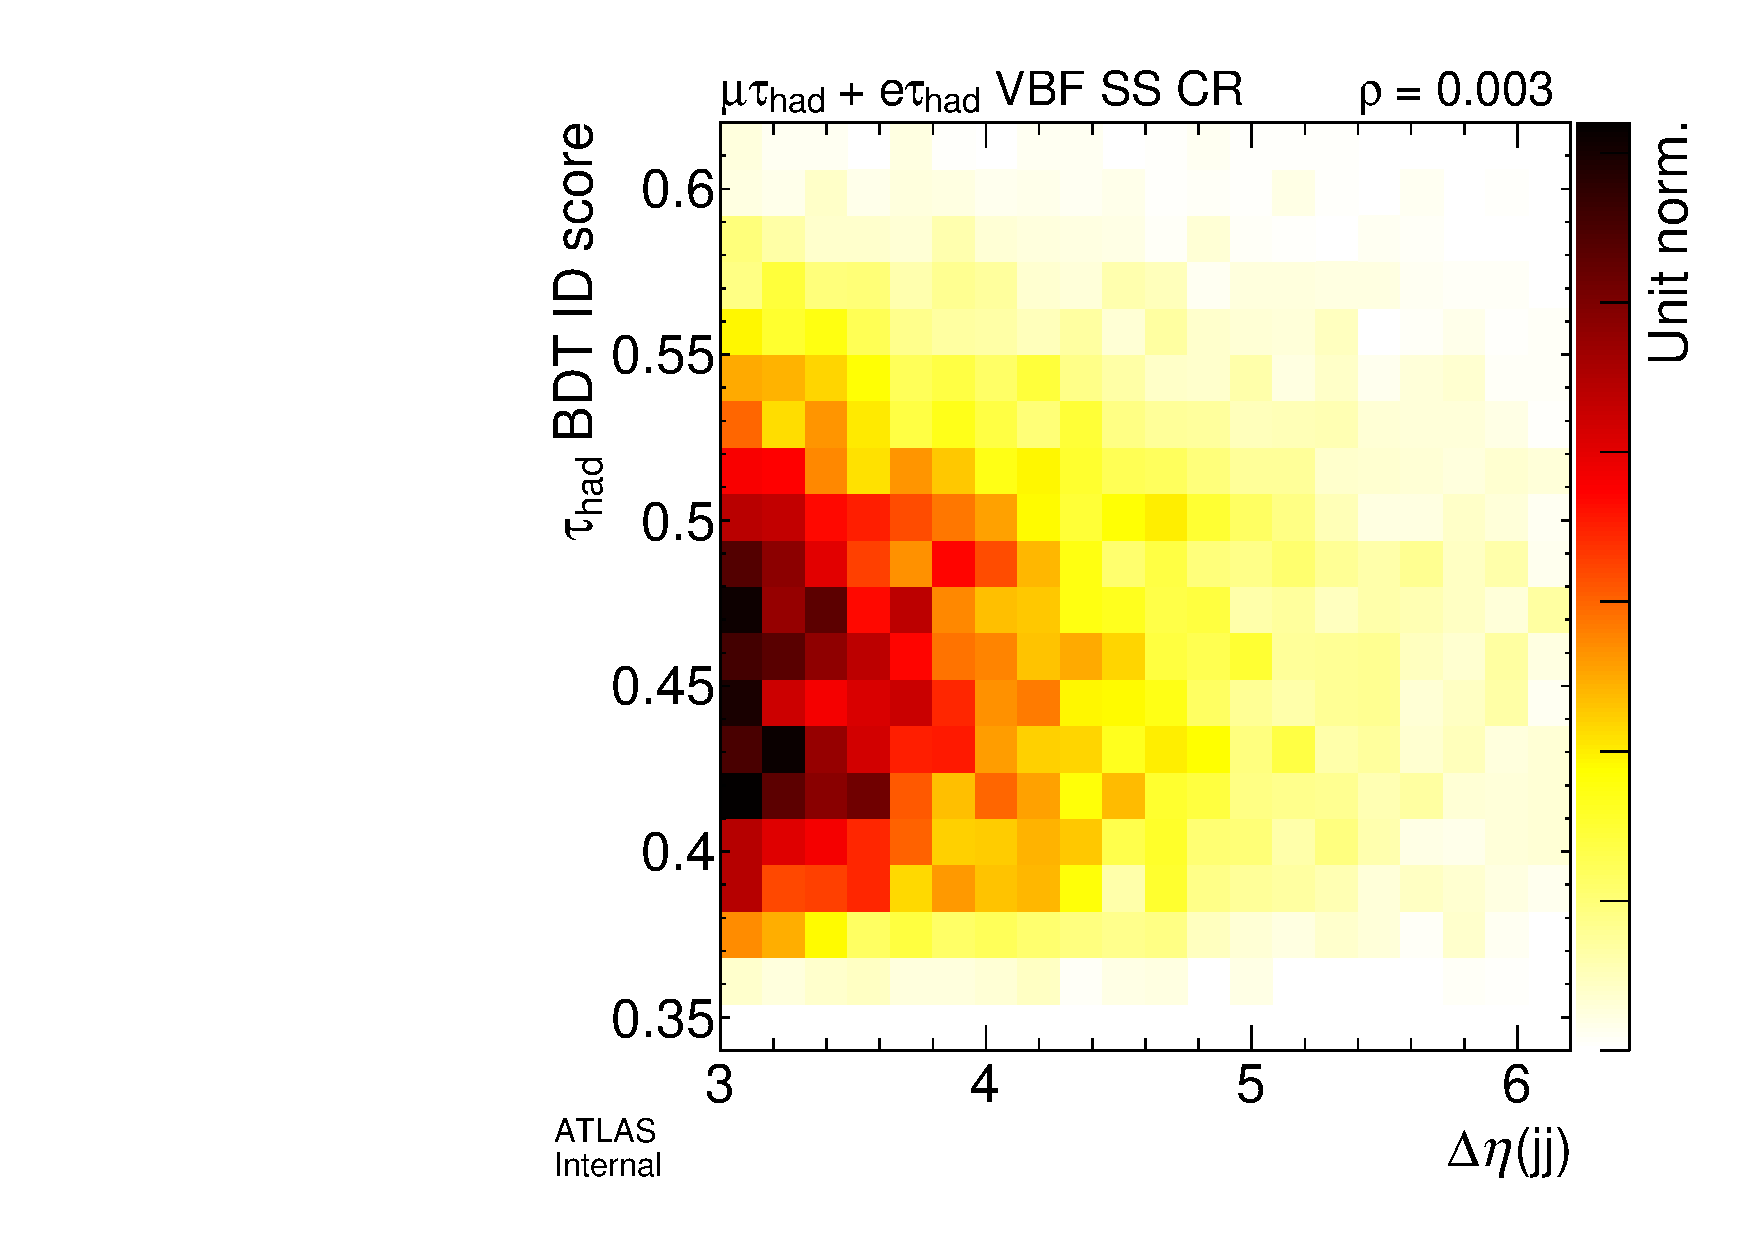
\includegraphics[width=0.32\textwidth]{figures/tauidcorrelations/tauid_vs_detajj}
  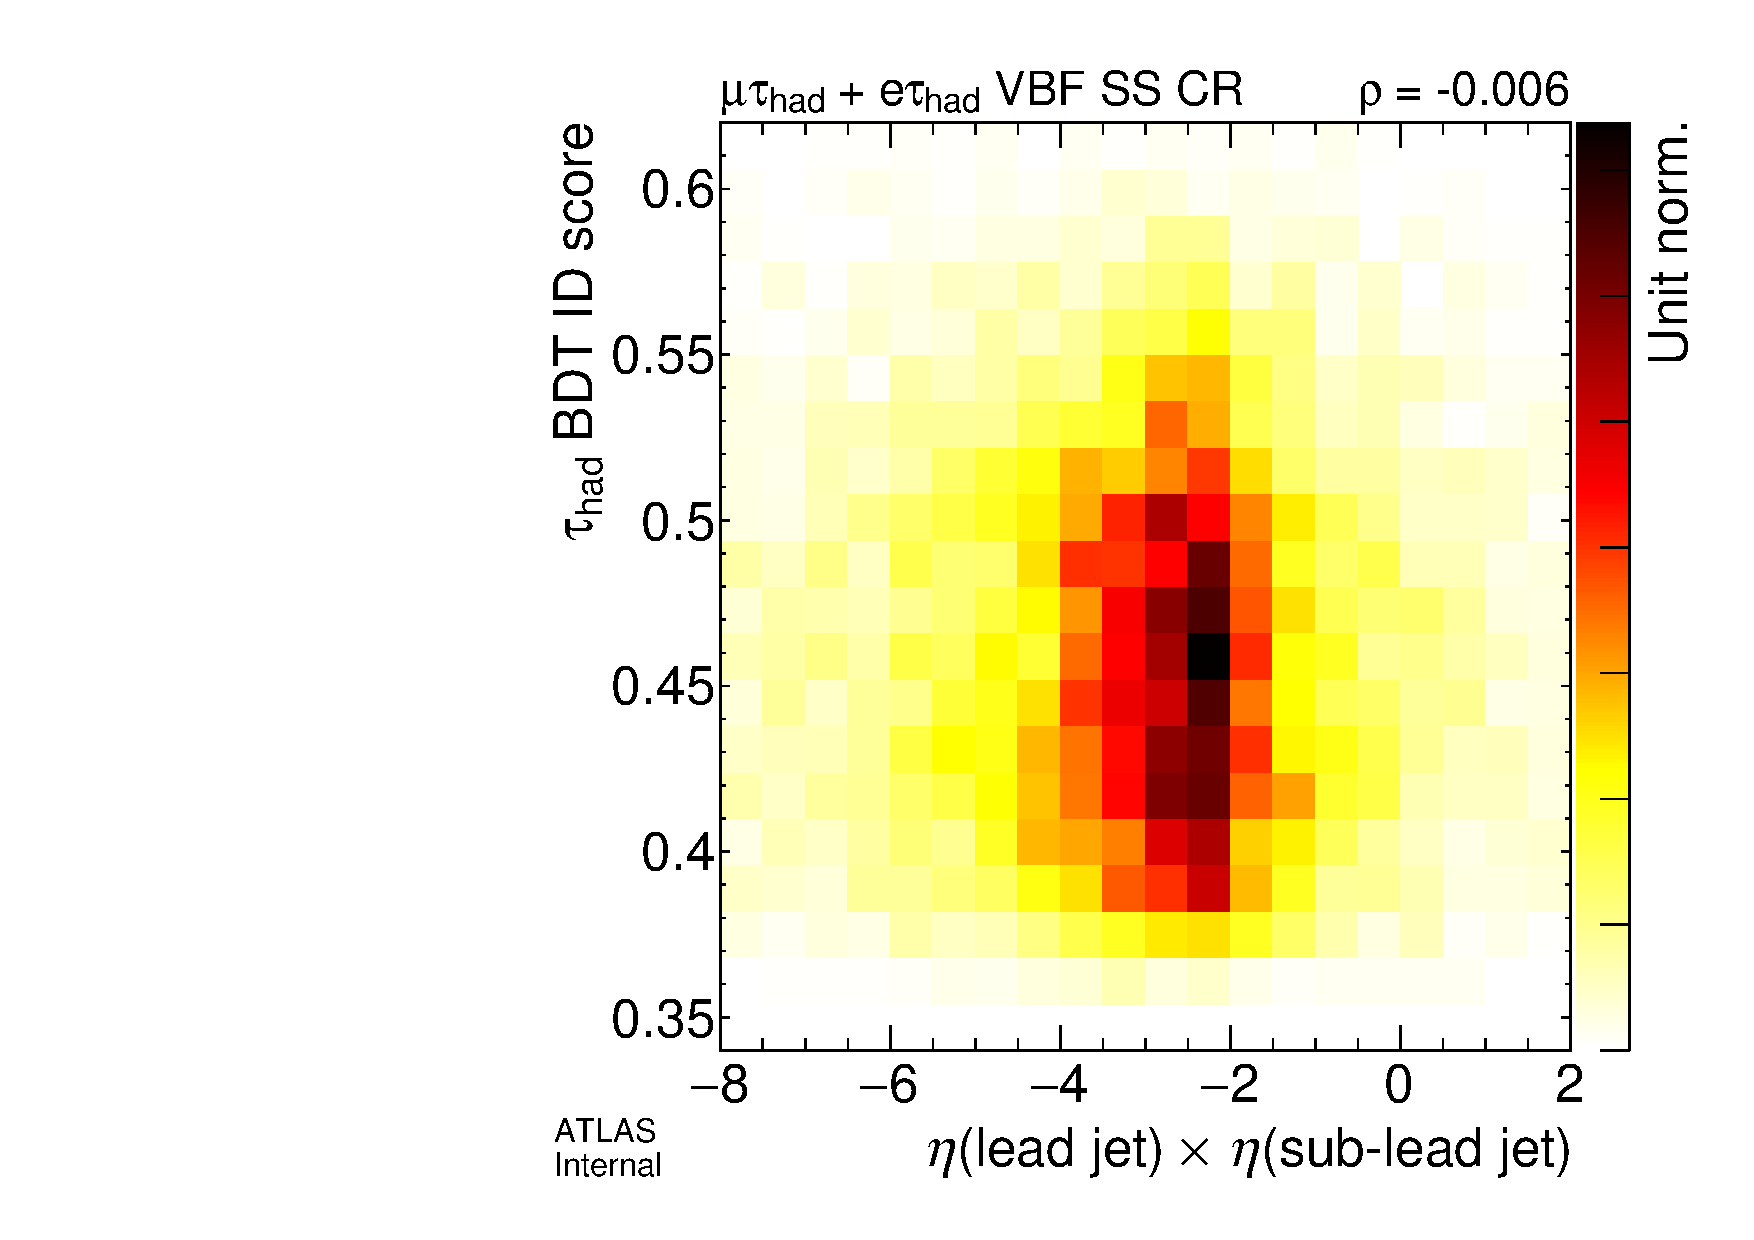
\includegraphics[width=0.32\textwidth]{figures/tauidcorrelations/tauid_vs_etaprod}
  % --------------
  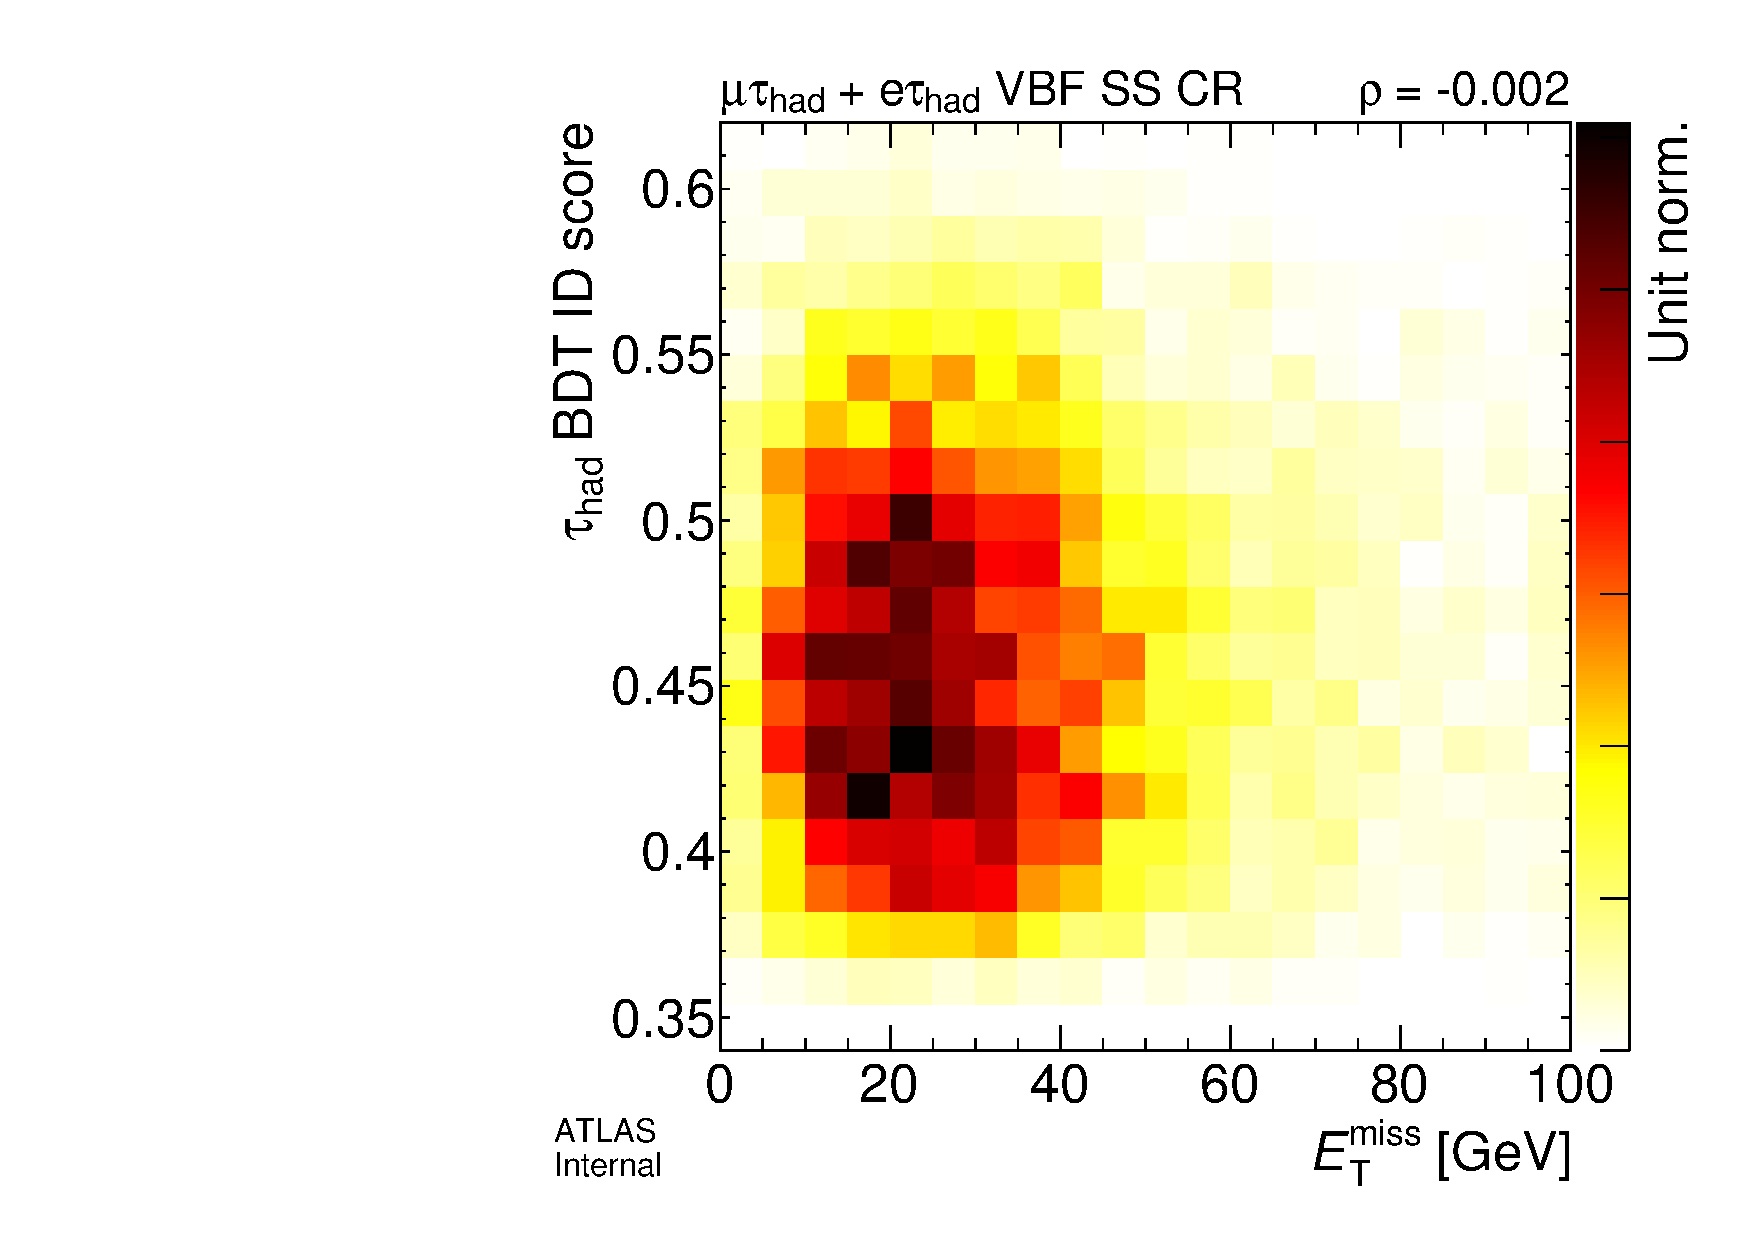
\includegraphics[width=0.32\textwidth]{figures/tauidcorrelations/tauid_vs_metet}
  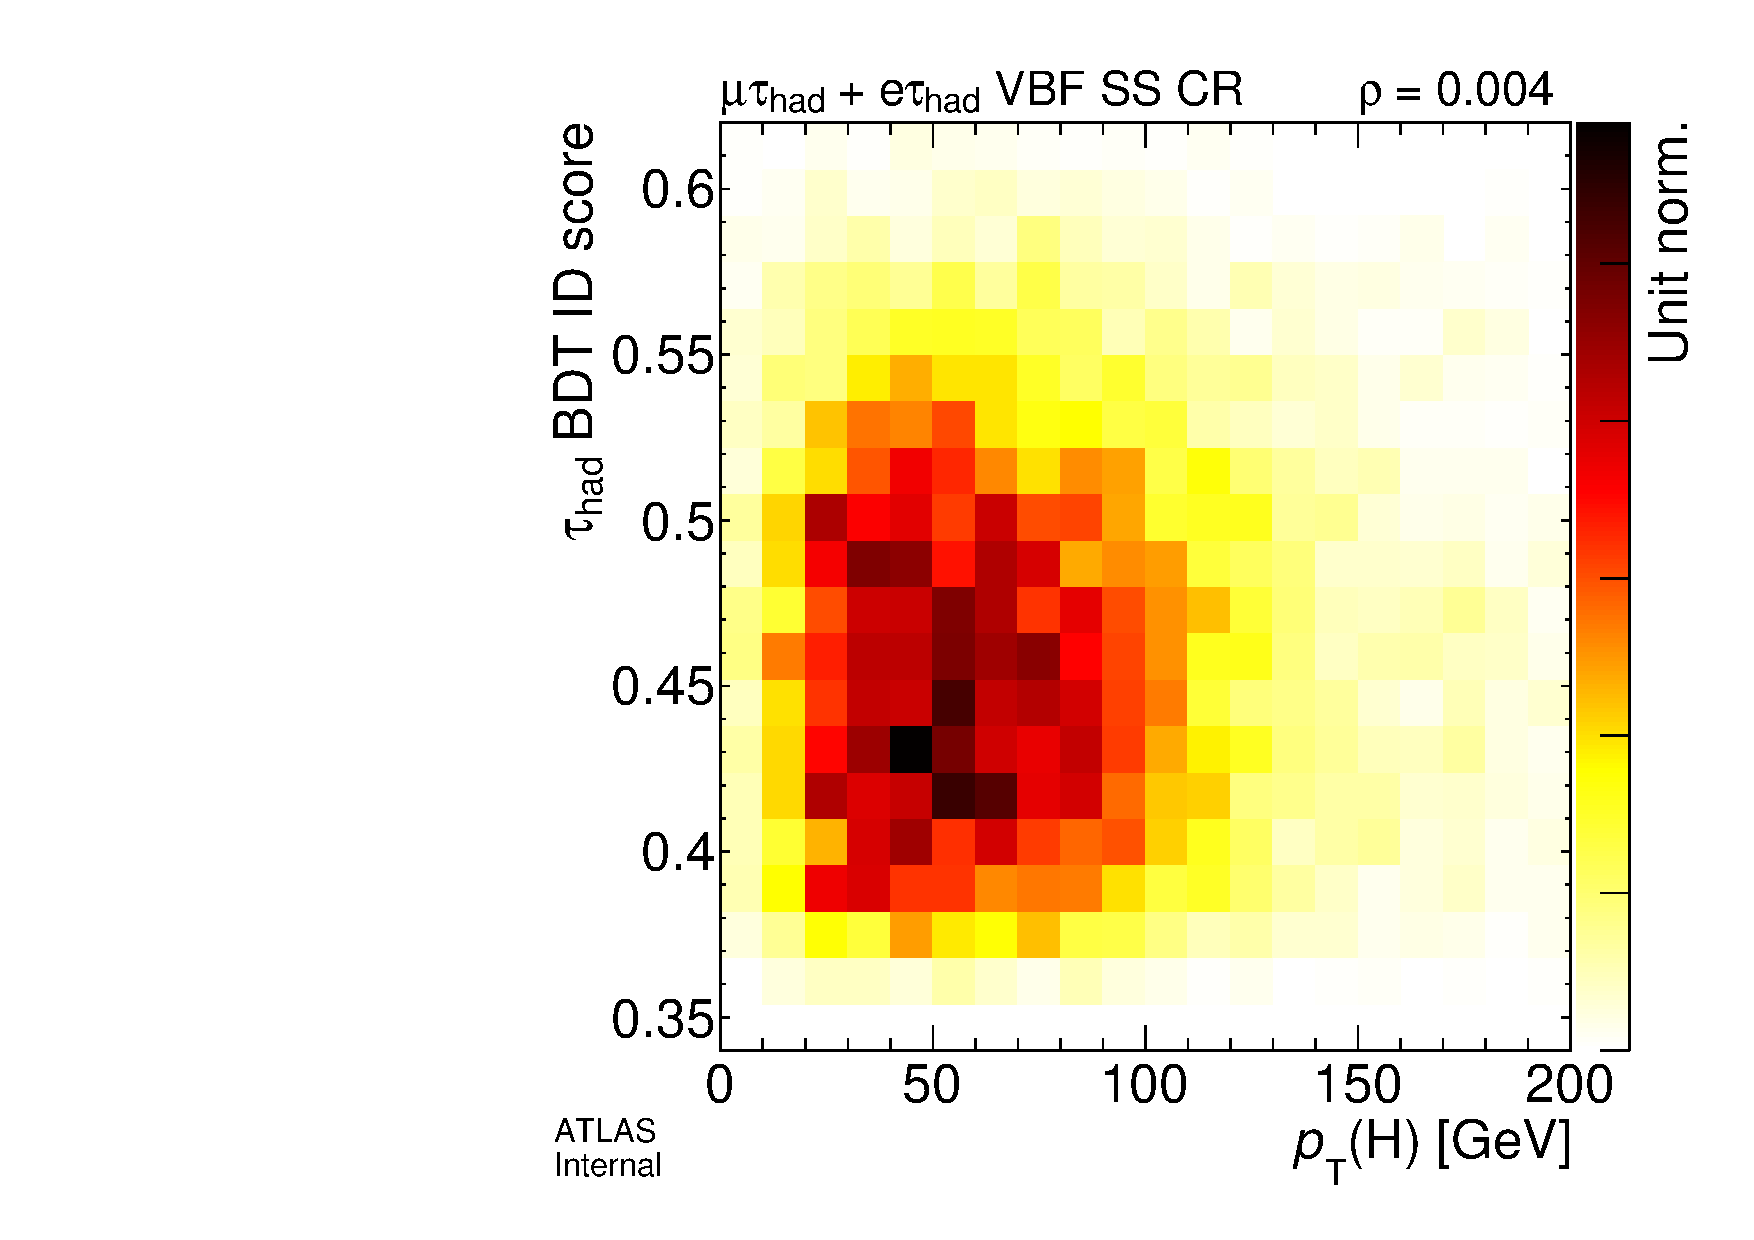
\includegraphics[width=0.32\textwidth]{figures/tauidcorrelations/tauid_vs_Hpt}
  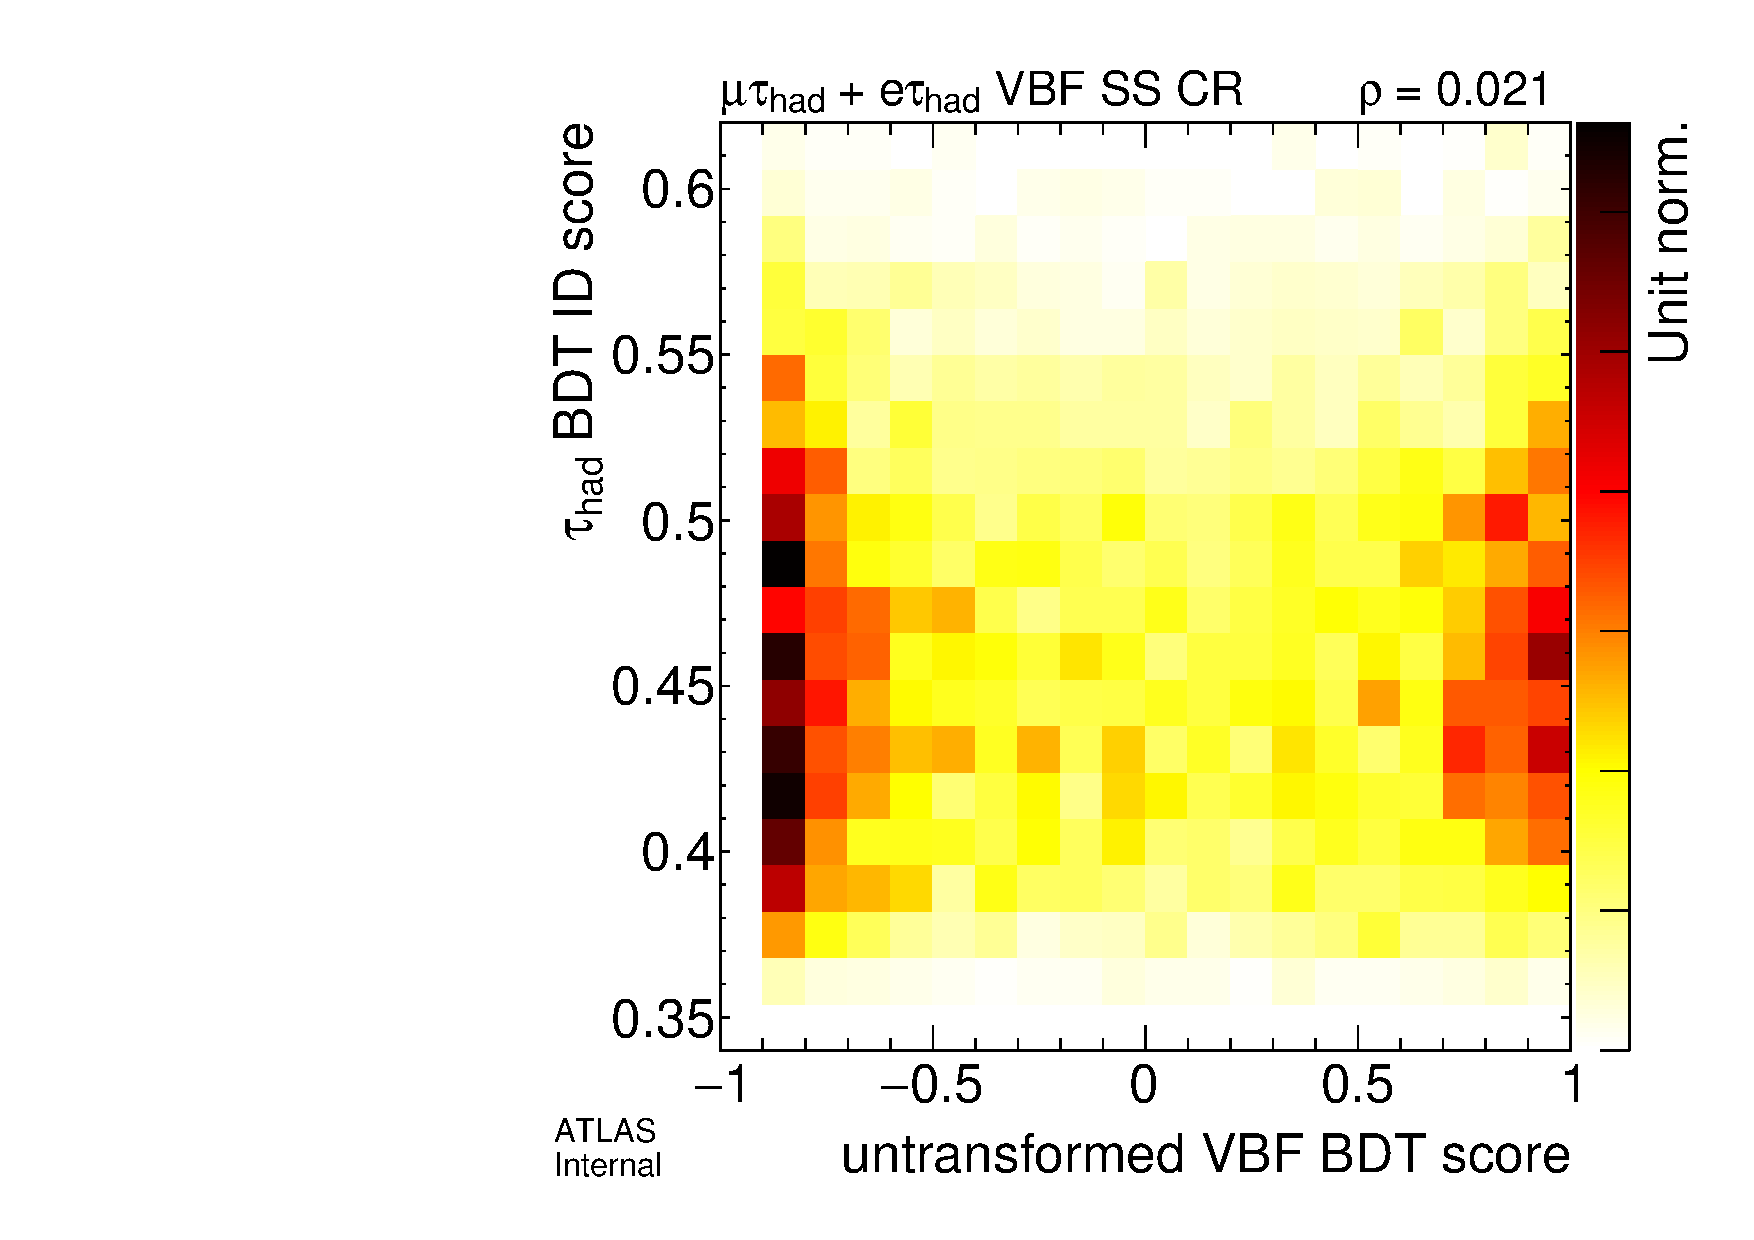
\includegraphics[width=0.32\textwidth]{figures/tauidcorrelations/tauid_vs_bdt}
  \caption{Correlations between the $\tauh$ BDT identification score and event kinematics in data events in the VBF same-sign region which fail $\tauh$ identification but fulfill all other requirements. No strong correlations are observed.}
  \label{fig:backgrounds-tauid-correlations}
\end{figure}

\clearpage

\begin{figure}[tp]
  \centering
  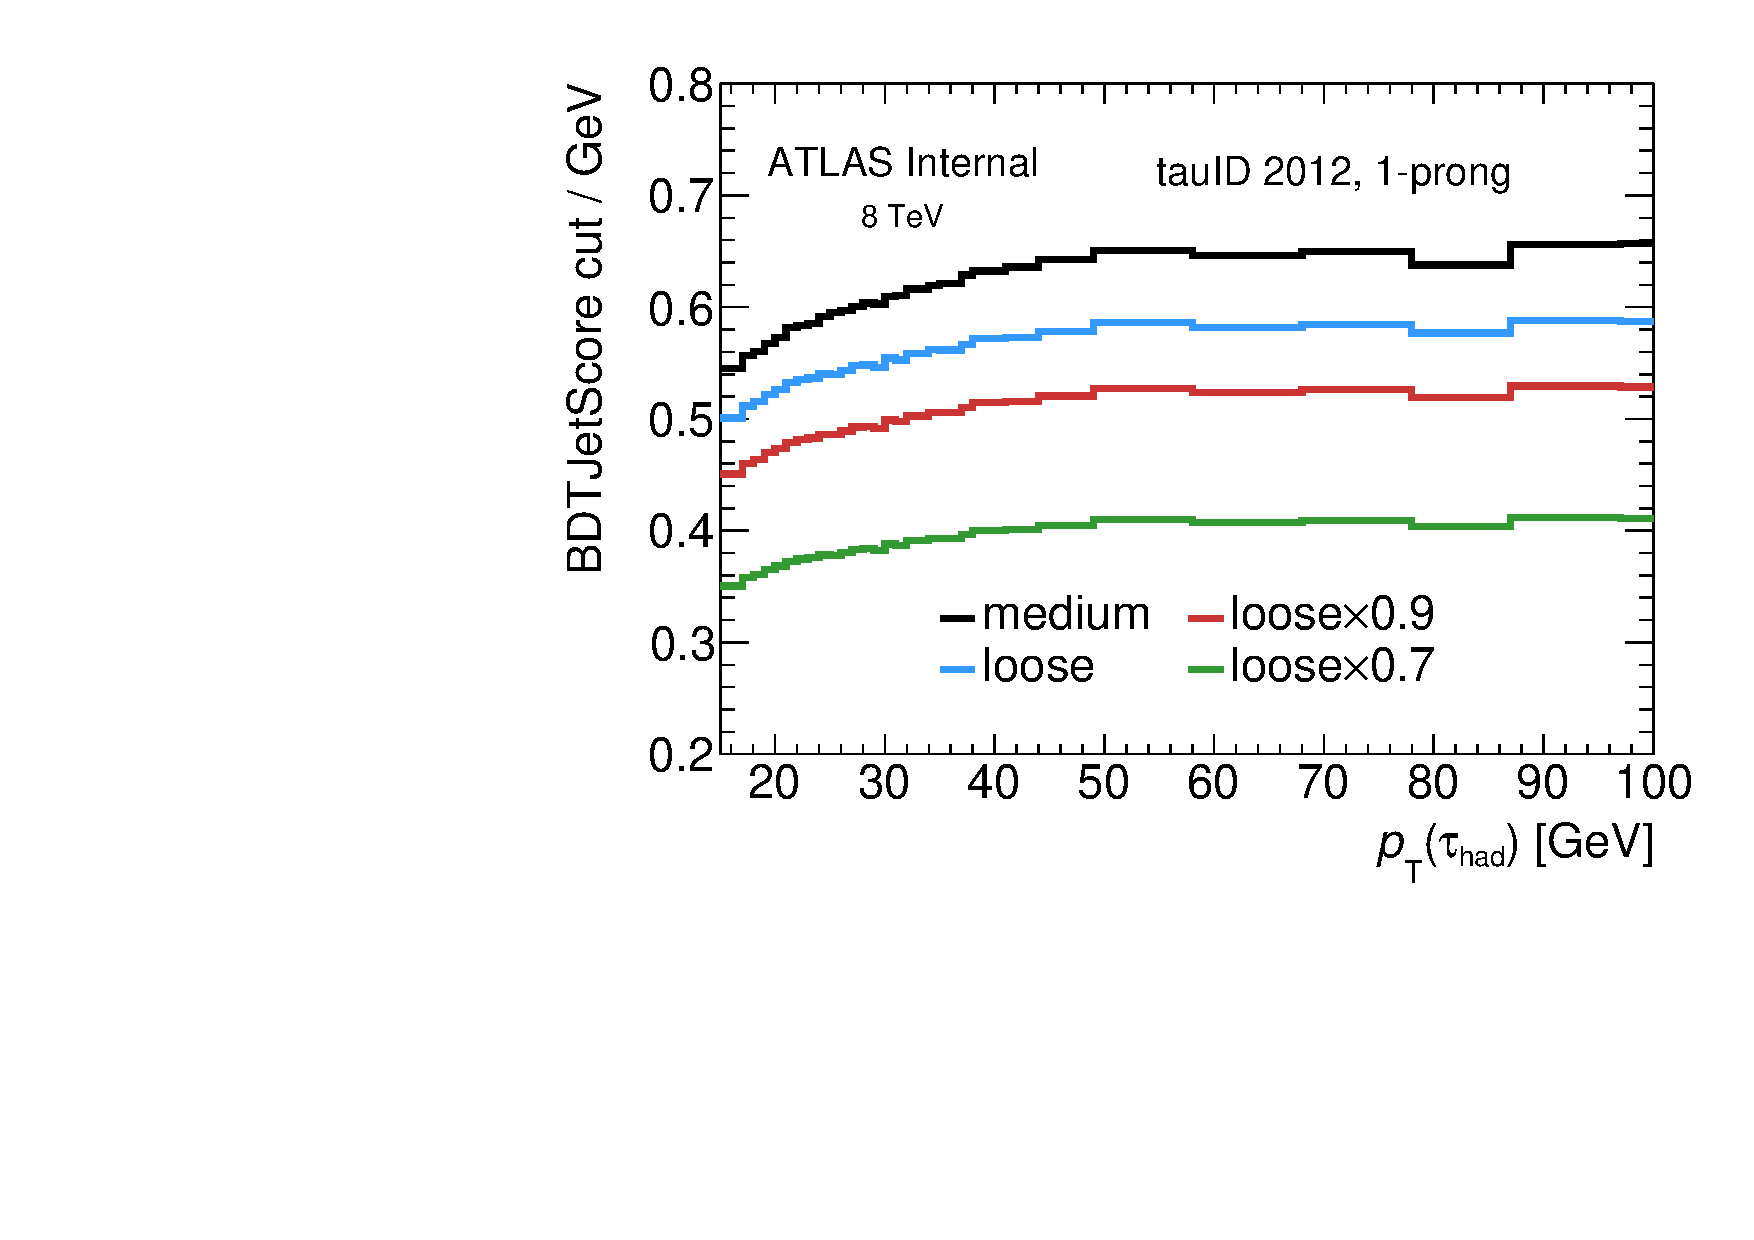
\includegraphics[width=0.48\textwidth]{figures/backgrounds/jetBDT-1p}
  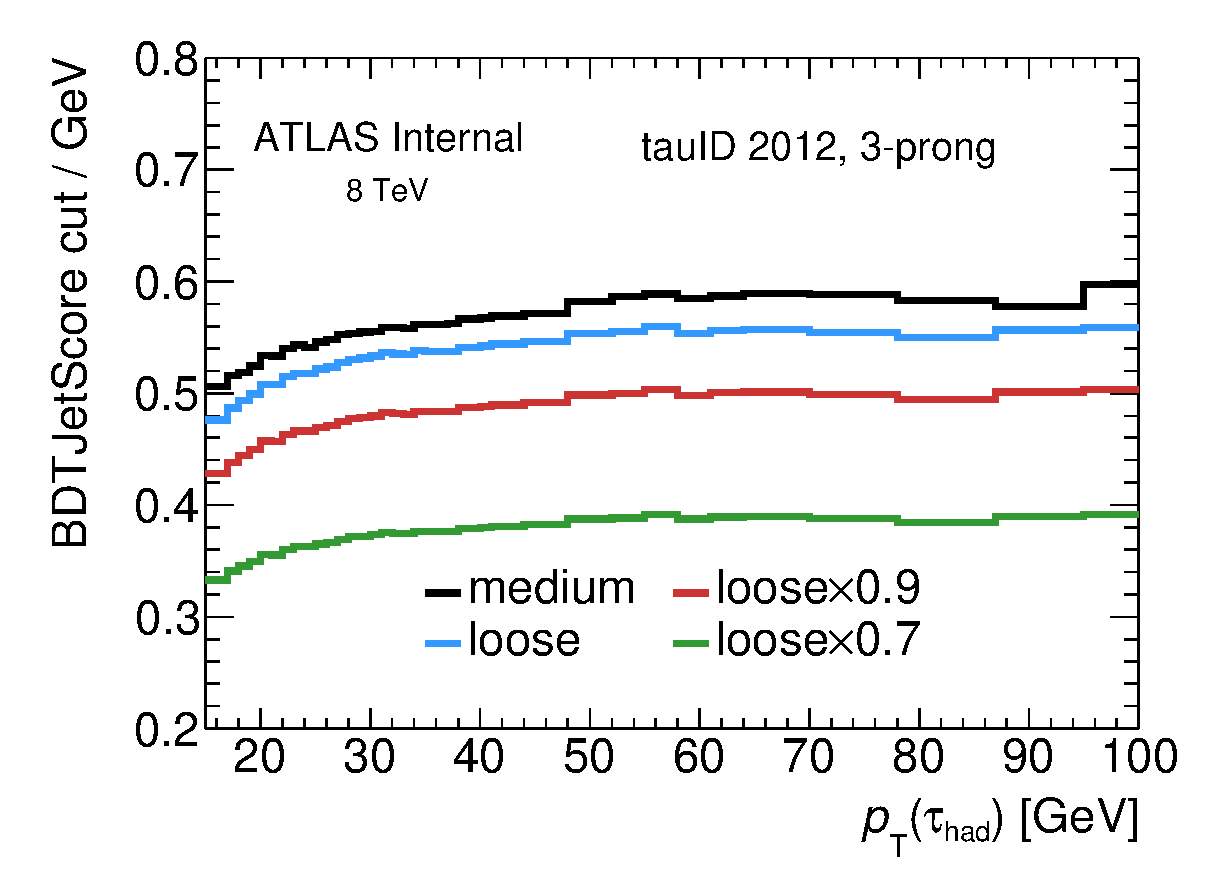
\includegraphics[width=0.48\textwidth]{figures/backgrounds/jetBDT-3p}
  \caption{Requirements on the $\tauh$ jet discriminant, which are defined to have constant signal efficiency as a function of $\pt(\tauh)$, of various operating points for 1-track $\tauh$ (left) and 3-track $\tauh$ (right).}
  \label{fig:backgrounds-workingpoints}
\end{figure}

\begin{figure}[tp]
  \centering
  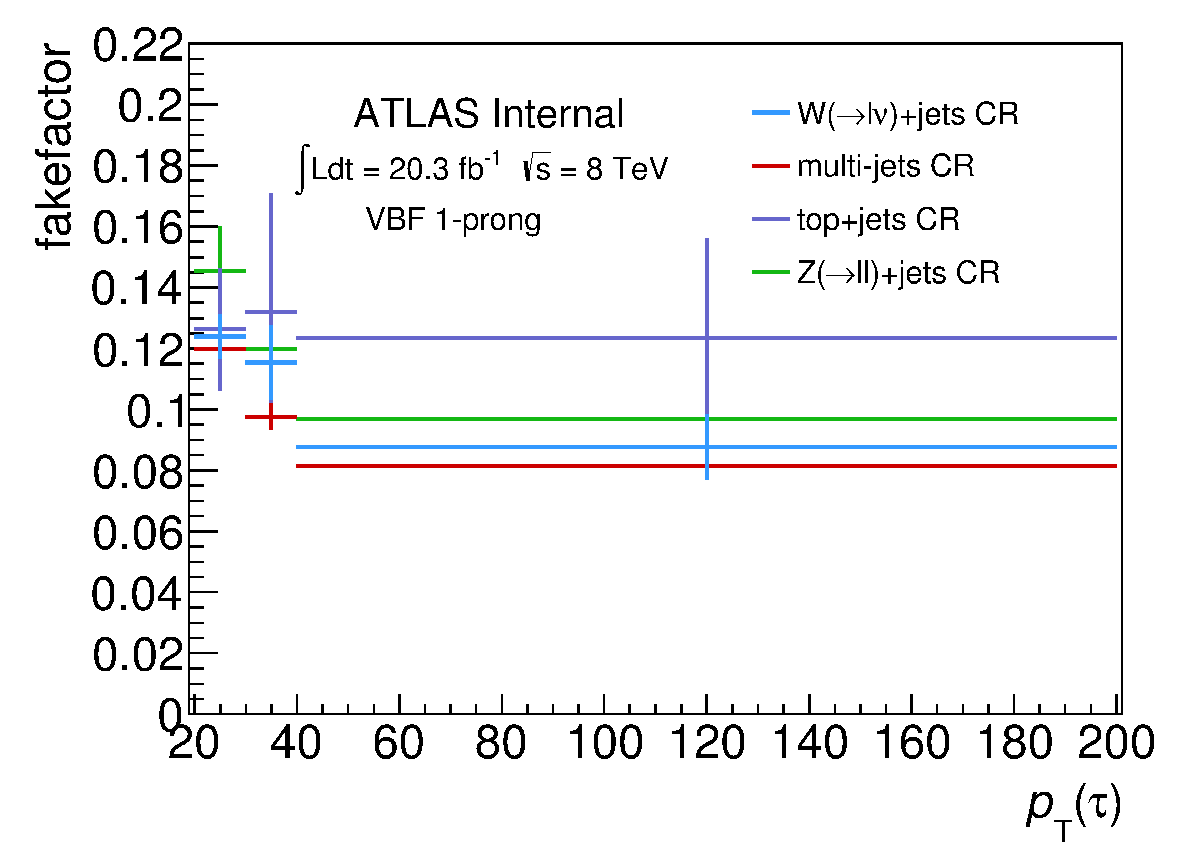
\includegraphics[width=0.48\textwidth]{figures/backgrounds/fakefactor_8TeV_vbf_1p_CRs}
  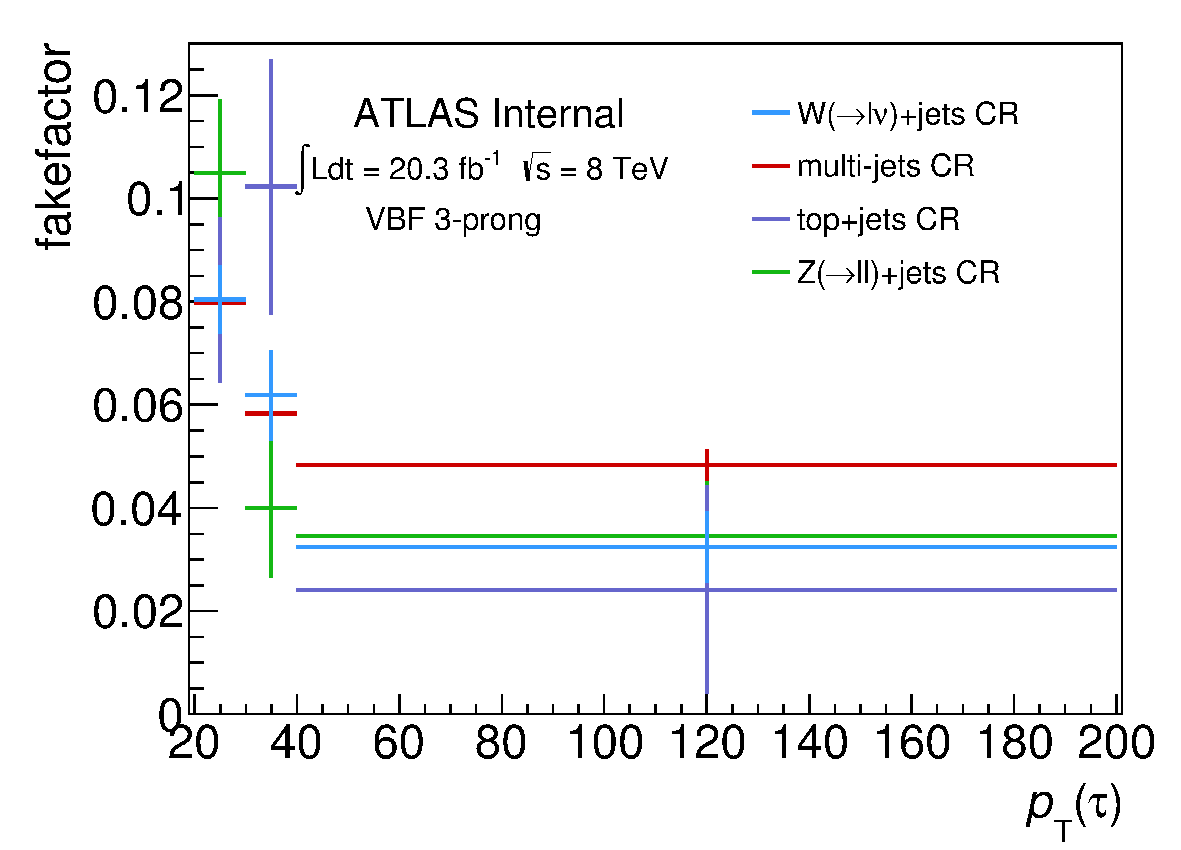
\includegraphics[width=0.48\textwidth]{figures/backgrounds/fakefactor_8TeV_vbf_3p_CRs}
  \caption{Fake factors in the VBF category measured in the various control regions in data for 1-track $\tauh$ (left) and 3-track $\tauh$ (right).}
  \label{fig:backgrounds-fakefactorsVBFCRs}
\end{figure}

\subsection{Composition of $\fakes$ in the SR}

\begin{figure}[tp]
  \centering
  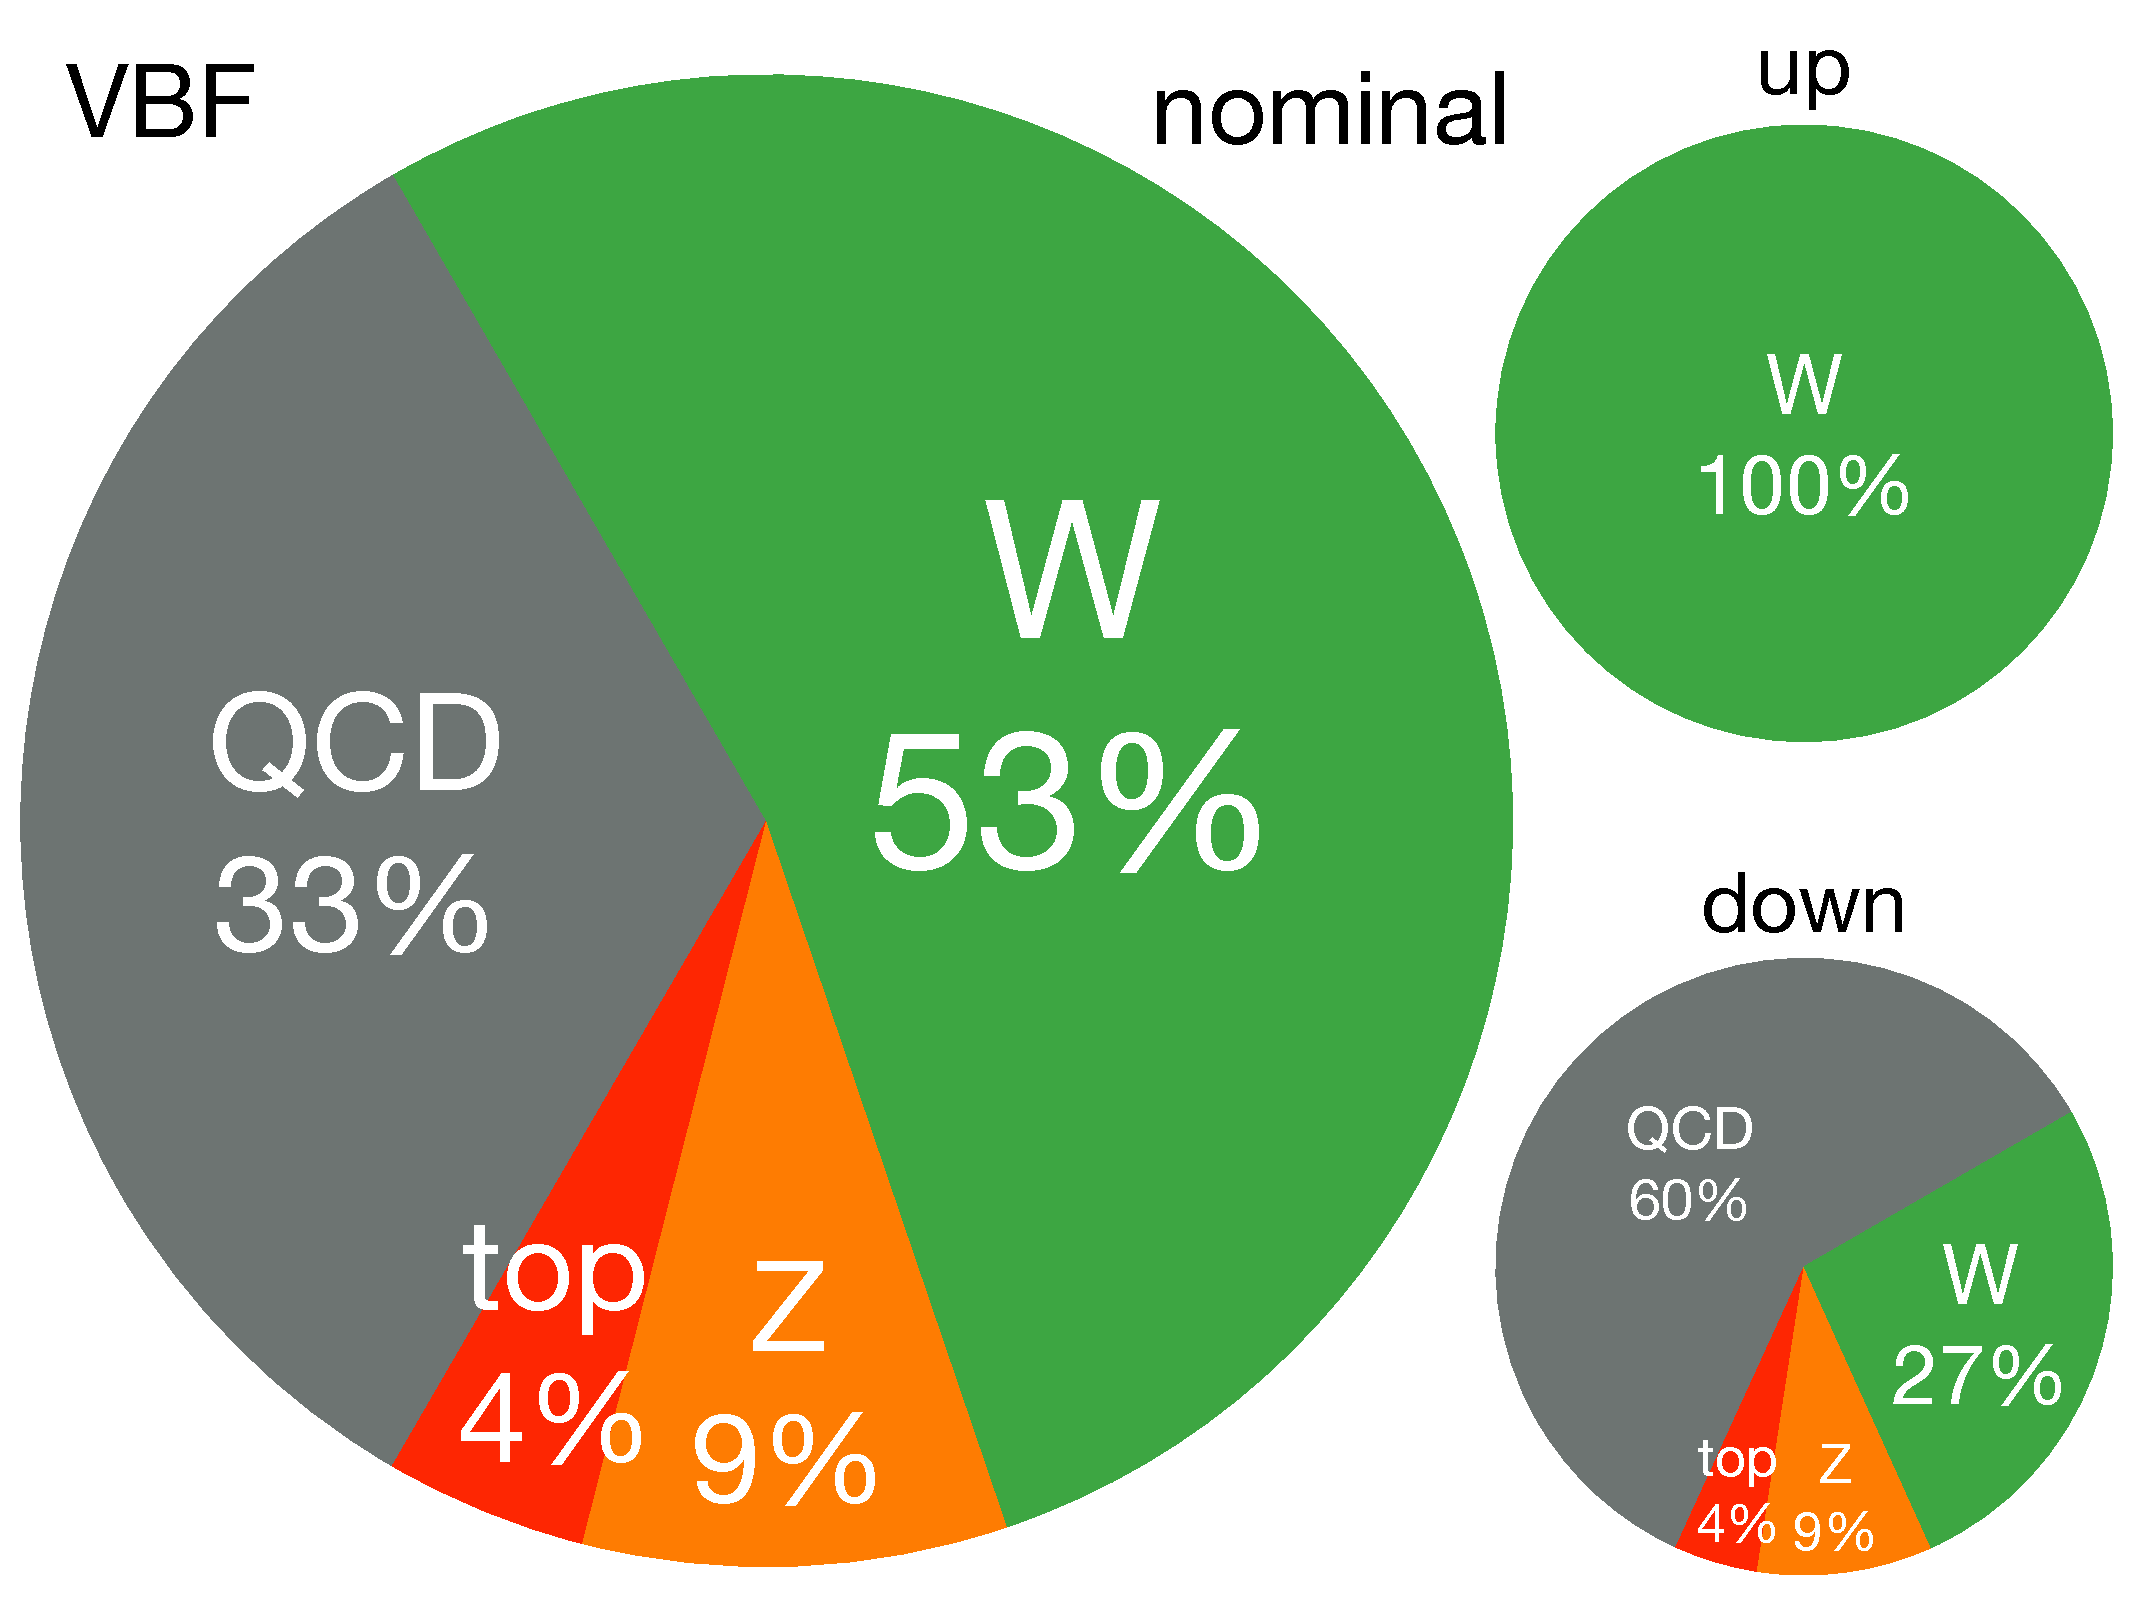
\includegraphics[width=0.90\textwidth]{figures/backgrounds/rx-vbf}
  \caption{A pie chart of the composition of $\fakes$ processes in the anti-identified CR as predicted by simulation and data (left) and the systematic variations on the composition (right).}
  \label{fig:backgrounds-rx-vbf}
\end{figure}

\clearpage

\begin{figure}[tp]
  \centering
  \includegraphics[width=0.32\textwidth]{figures/rx/vbf-mvaSR/tau-pt}
  \includegraphics[width=0.32\textwidth]{figures/rx/vbf-mvaSR/tau-eta}
  \includegraphics[width=0.32\textwidth]{figures/rx/vbf-mvaSR/tau-numTrack}
  % --------------
  \includegraphics[width=0.32\textwidth]{figures/rx/vbf-mvaSR/lep-pt-hi}
  \includegraphics[width=0.32\textwidth]{figures/rx/vbf-mvaSR/lep-eta}
  \includegraphics[width=0.32\textwidth]{figures/rx/vbf-mvaSR/taulep-dR}
  % --------------
  \includegraphics[width=0.32\textwidth]{figures/rx/vbf-mvaSR/met-pt-hi}
  \includegraphics[width=0.32\textwidth]{figures/rx/vbf-mvaSR/mMMC}
  \includegraphics[width=0.32\textwidth]{figures/rx/vbf-mvaSR/mT}
  % --------------
  \includegraphics[width=0.32\textwidth]{figures/rx/vbf-mvaSR/met-phi-centrality}
  \includegraphics[width=0.32\textwidth]{figures/rx/vbf-mvaSR/H-pt-hi}
  \includegraphics[width=0.32\textwidth]{figures/rx/vbf-mvaSR/mvis}
  \caption{The composition of $\fakes$ processes in the anti-identified CR as predicted by simulation and data as a function of event kinematics.}
  \label{fig:backgrounds-rx-vbf-taus}
\end{figure}

\clearpage

\begin{figure}[tp]
  \includegraphics[width=0.32\textwidth]{figures/rx/vbf-mvaSR/jet-1-pt}
  \includegraphics[width=0.32\textwidth]{figures/rx/vbf-mvaSR/jet-1-eta}
  \includegraphics[width=0.32\textwidth]{figures/rx/vbf-mvaSR/jets-dphi}
  % --------------
  \includegraphics[width=0.32\textwidth]{figures/rx/vbf-mvaSR/jet-2-pt}
  \includegraphics[width=0.32\textwidth]{figures/rx/vbf-mvaSR/jet-2-eta}
  \includegraphics[width=0.32\textwidth]{figures/rx/vbf-mvaSR/jets-deta}
  % --------------
  \includegraphics[width=0.32\textwidth]{figures/rx/vbf-mvaSR/jets-etaprod}
  \includegraphics[width=0.32\textwidth]{figures/rx/vbf-mvaSR/lep-eta-centrality}
  \includegraphics[width=0.32\textwidth]{figures/rx/vbf-mvaSR/system-pt}
  % --------------
  \includegraphics[width=0.32\textwidth]{figures/rx/vbf-mvaSR/n-jets30}
  \includegraphics[width=0.32\textwidth]{figures/rx/vbf-mvaSR/dijet-m-veryhigh}
  \includegraphics[width=0.32\textwidth]{figures/rx/vbf-mvaSR/BDTEve-VBF}
  \caption{The composition of $\fakes$ processes in the anti-identified CR as predicted by simulation and data as a function of event kinematics.}
  \label{fig:backgrounds-rx-vbf-jets}
\end{figure}

\begin{figure}[tp]
  \centering
  \includegraphics[width=0.48\textwidth]{figures/backgrounds/fakefactor_8TeV_vbf_1p_mix}
  \includegraphics[width=0.48\textwidth]{figures/backgrounds/fakefactor_8TeV_vbf_3p_mix}
  \caption{Fake factors in the VBF category mixed from the various control regions in data for 1-track $\tauh$ (left) and 3-track $\tauh$ (right). Statistical and systematic uncertainties are shown.}
  \label{fig:backgrounds-fakefactorsVBFmix}
\end{figure}

\clearpage

\subsection{Validation}

\begin{figure}[tp]
  \centering
  \includegraphics[width=0.90\textwidth]{figures/backgrounds/regions-cartoon}
  \caption{Cartoon of the signal, control, and validation regions used which are used in the $\fakes$ estimate.}
  \label{fig:backgrounds-regions}
\end{figure}

\clearpage

\begin{figure}[tp]
  \centering
  \includegraphics[width=0.32\textwidth]{figures/analysis/vbf-SSXCR/tau-pt}
  \includegraphics[width=0.32\textwidth]{figures/analysis/vbf-SSXCR/tau-eta}
  \includegraphics[width=0.32\textwidth]{figures/analysis/vbf-SSXCR/tau-numTrack}
  % --------------
  \includegraphics[width=0.32\textwidth]{figures/analysis/vbf-SSXCR/lep-pt-hi}
  \includegraphics[width=0.32\textwidth]{figures/analysis/vbf-SSXCR/lep-eta}
  \includegraphics[width=0.32\textwidth]{figures/analysis/vbf-SSXCR/taulep-dR}
  % --------------
  \includegraphics[width=0.32\textwidth]{figures/analysis/vbf-SSXCR/met-pt-hi}
  \includegraphics[width=0.32\textwidth]{figures/analysis/vbf-SSXCR/mMMC}
  \includegraphics[width=0.32\textwidth]{figures/analysis/vbf-SSXCR/mT}
  % --------------
  \includegraphics[width=0.32\textwidth]{figures/analysis/vbf-SSXCR/met-phi-centrality}
  \includegraphics[width=0.32\textwidth]{figures/analysis/vbf-SSXCR/H-pt-hi}
  \includegraphics[width=0.32\textwidth]{figures/analysis/vbf-SSXCR/mvis}
  \caption{Comparison of data and $\fakes$ prediction in the same-sign validation region for various event kinematics. The purity of $\fakes$ is $\approx\! 97\%$. Only statistical uncertainties are shown, and no sign of systematic bias is observed.}
  \label{fig:backgrounds-SSXCR-taus}
\end{figure}

\clearpage
\begin{figure}[tp]
  \includegraphics[width=0.32\textwidth]{figures/analysis/vbf-SSXCR/jet-1-pt}
  \includegraphics[width=0.32\textwidth]{figures/analysis/vbf-SSXCR/jet-1-eta}
  \includegraphics[width=0.32\textwidth]{figures/analysis/vbf-SSXCR/jets-dphi}
  % --------------
  \includegraphics[width=0.32\textwidth]{figures/analysis/vbf-SSXCR/jet-2-pt}
  \includegraphics[width=0.32\textwidth]{figures/analysis/vbf-SSXCR/jet-2-eta}
  \includegraphics[width=0.32\textwidth]{figures/analysis/vbf-SSXCR/jets-deta}
  % --------------
  \includegraphics[width=0.32\textwidth]{figures/analysis/vbf-SSXCR/jets-etaprod}
  \includegraphics[width=0.32\textwidth]{figures/analysis/vbf-SSXCR/lep-eta-centrality}
  \includegraphics[width=0.32\textwidth]{figures/analysis/vbf-SSXCR/system-pt}
  % --------------
  \includegraphics[width=0.32\textwidth]{figures/analysis/vbf-SSXCR/n-jets30}
  \includegraphics[width=0.32\textwidth]{figures/analysis/vbf-SSXCR/dijet-m-veryhigh}
  \includegraphics[width=0.32\textwidth]{figures/analysis/vbf-SSXCR/BDTEve-VBF}
  \caption{Comparison of data and $\fakes$ prediction in the same-sign validation region for various event kinematics. The purity of $\fakes$ is $\approx\! 97\%$. Only statistical uncertainties are shown, and no sign of systematic bias is observed.}
  \label{fig:backgrounds-SSXCR-jets}
\end{figure}

\clearpage

\begin{figure}[tp]
  \centering
  \includegraphics[width=0.32\textwidth]{figures/analysis/vbf-MCXSR/tau-pt}
  \includegraphics[width=0.32\textwidth]{figures/analysis/vbf-MCXSR/tau-eta}
  \includegraphics[width=0.32\textwidth]{figures/analysis/vbf-MCXSR/tau-numTrack}
  % --------------
  \includegraphics[width=0.32\textwidth]{figures/analysis/vbf-MCXSR/lep-pt-hi}
  \includegraphics[width=0.32\textwidth]{figures/analysis/vbf-MCXSR/lep-eta}
  \includegraphics[width=0.32\textwidth]{figures/analysis/vbf-MCXSR/taulep-dR}
  % --------------
  \includegraphics[width=0.32\textwidth]{figures/analysis/vbf-MCXSR/met-pt-hi}
  \includegraphics[width=0.32\textwidth]{figures/analysis/vbf-MCXSR/mMMC}
  \includegraphics[width=0.32\textwidth]{figures/analysis/vbf-MCXSR/mT}
  % --------------
  \includegraphics[width=0.32\textwidth]{figures/analysis/vbf-MCXSR/met-phi-centrality}
  \includegraphics[width=0.32\textwidth]{figures/analysis/vbf-MCXSR/H-pt-hi}
  \includegraphics[width=0.32\textwidth]{figures/analysis/vbf-MCXSR/mvis}
  \caption{Comparison of the prediction of identified taus and the $\fakes$ prediction, both in simulation, in the signal region for various event kinematics. Only statistical uncertainties are shown, and no sign of systematic bias is observed.}
  \label{fig:backgrounds-MCXSR-taus}
\end{figure}

\clearpage

\begin{figure}[tp]
  \includegraphics[width=0.32\textwidth]{figures/analysis/vbf-MCXSR/jet-1-pt}
  \includegraphics[width=0.32\textwidth]{figures/analysis/vbf-MCXSR/jet-1-eta}
  \includegraphics[width=0.32\textwidth]{figures/analysis/vbf-MCXSR/jets-dphi}
  % --------------
  \includegraphics[width=0.32\textwidth]{figures/analysis/vbf-MCXSR/jet-2-pt}
  \includegraphics[width=0.32\textwidth]{figures/analysis/vbf-MCXSR/jet-2-eta}
  \includegraphics[width=0.32\textwidth]{figures/analysis/vbf-MCXSR/jets-deta}
  % --------------
  \includegraphics[width=0.32\textwidth]{figures/analysis/vbf-MCXSR/jets-etaprod}
  \includegraphics[width=0.32\textwidth]{figures/analysis/vbf-MCXSR/lep-eta-centrality}
  \includegraphics[width=0.32\textwidth]{figures/analysis/vbf-MCXSR/system-pt}
  % --------------
  \includegraphics[width=0.32\textwidth]{figures/analysis/vbf-MCXSR/n-jets30}
  \includegraphics[width=0.32\textwidth]{figures/analysis/vbf-MCXSR/dijet-m-high}
  \includegraphics[width=0.32\textwidth]{figures/analysis/vbf-MCXSR/BDTEve-VBF}
  \caption{Comparison of the prediction of identified taus and the $\fakes$ prediction, both in simulation, in the signal region for various event kinematics. Only statistical uncertainties are shown, and no sign of systematic bias is observed.}
  \label{fig:backgrounds-MCXSR-jets}
\end{figure}

\clearpage

\subsection{Uncertainties}

\begin{figure}[tp]
  \includegraphics[width=0.90\textwidth]{figures/uncertainties/uncertainties_lephad_paper14_8TeV_fakes_VBF}
  \caption{The fractional uncertainty on the $\fakes$ prediction in each bin of the VBF category.}
  \label{fig:backgrounds-uncertainties-fakes}
\end{figure}

\clearpage

\section{top, $\Zll$, diboson}
\label{sec:backgrounds-others}

\section{$\Htautau$}
\label{sec:backgrounds-htautau}

\subsection{Generators}

\subsection{Uncertainties}

\begin{figure}[tp]
  \includegraphics[width=0.90\textwidth]{figures/uncertainties/uncertainties_lephad_paper14_8TeV_VBFH125_JES_VBF}
  \caption{The fractional uncertainty on the VBF $\Htautaulh$ prediction in each bin of the VBF category for uncertainties pertaining to the jet energy scale.}
  \label{fig:backgrounds-uncertainties-vbfjes}
\end{figure}

\begin{figure}[tp]
  \includegraphics[width=0.90\textwidth]{figures/uncertainties/uncertainties_lephad_paper14_8TeV_VBFH125_other_VBF}
  \caption{The fractional uncertainty on the VBF $\Htautaulh$ prediction in each bin of the VBF category for uncertainties pertaining to $\tauh$ performance, theory, and the luminosity.}
  \label{fig:backgrounds-uncertainties-vbfother}
\end{figure}

